\documentclass[titlepage,a4paper,oneside,onecolumn,12pt]{report}
% \documentclass[titlepage,a4paper,oneside,onecolumn,12pt,draft]{report}

\usepackage[utf8]{inputenc}
\usepackage[T1]{fontenc}
\usepackage[pdftex,
            pdfauthor={Rodolfo Pereira Araujo},
            pdftitle={Estratégias de exploração de vizinhança com GPU para problemas de otimização},
            pdfsubject={Pesquisa Operacional},
            pdfkeywords={Meta-heurística, Busca Local, Dataflow, Graphics Processing Unit, Variable},
            pdfproducer={Latex with hyperref, or other system},
            pdfcreator={pdflatex}]{hyperref}
\usepackage[top=3cm, bottom=2cm, left=3cm, right=2cm]{geometry}
\usepackage[table,xcdraw]{xcolor}
\usepackage[alf]{abntex2cite}
\usepackage{pgfplotstable}
\usepackage{pgfplots}
\usepackage[brazil]{babel}
\usepackage{amssymb,amsmath,amsthm}
\usepackage{dsfont}
\usepackage[section]{placeins}
\usepackage[ruled]{algorithm} %[ruled]
\usepackage[noend]{algpseudocode}
\usepackage[singlelinecheck=false, justification=raggedright, labelsep=endash]{caption}
\usepackage{multirow}
\usepackage{makecell}
\usepackage{mathtools}
\usepackage{fancyhdr}
\usepackage{relsize}
\usepackage{setspace}

\usepackage{icomma}
\usepackage{silence}
\usepackage{etoolbox}
\usepackage{tocloft}
\usepackage{titlesec}
\usepackage{chngcntr}
\usepackage{indentfirst}
\usepackage[nottoc,notlot,notlof]{tocbibind}
\usepackage{pdfpages}
\usepackage{centernot}
\usepackage{minted}
\usepackage{ulem}

\newtheorem{theorem}{Teorema}
\newtheorem{corolario}[theorem]{Corolário}
\newtheorem{lema}[theorem]{Lema}
\newtheorem{proposicao}[theorem]{Proposição}

\usepackage{mathtools} % Bonus

\renewcommand{\cftchapleader}{\cftdotfill{\cftdotsep}}

\setcounter{tocdepth}{5} %aparece tudo no sumario
\setcounter{secnumdepth}{5} %aparece tudo no sumario

\captionsetup[figure]{font=normalsize,labelfont=normalsize} %font 12 em caption
\captionsetup[table]{font=normalsize,labelfont=normalsize} %font 12 em caption
\usepackage[justification=raggedright, singlelinecheck=false,]{subcaption}
% \usepackage[justification=raggedright, singlelinecheck=false,]{subfig}
% \captionsetup[subfigure]{font=normalsize,labelfont=normalsize} %font 10 em subcaption
 
\MakeRobust{\Call} %algoritmo
\algrenewcommand\Return{\State \algorithmicreturn{} }%
\newcommand*\Let[2]{\State #1 $\gets$ #2} %atribuição
\algdef{SE}[DOWHILE]{Do}{doWhile}{\algorithmicdo}[1]{\algorithmicwhile\ #1} %define do-while
\renewcommand{\algorithmicrequire}{\textbf{Requerimento:}}
\renewcommand{\algorithmicensure}{\textbf{Observação:}}

\renewcommand{\algorithmicreturn}{\textbf{retorna}}
\renewcommand{\algorithmicfunction}{\textbf{função}}
\renewcommand{\algorithmicprocedure}{\textbf{procedimento}}
\newcommand{\noProcedure}[2]{\Statex{\textbf{procedimento }#1(#2)}}
\newcommand{\noFunction}[2]{\Statex{\textbf{função }#1(#2)}}


%% Miscelânea: inicializadores e terminadores de blocos, comandos diversos

\renewcommand{\algorithmicdo}{\textbf{fa\c{c}a}}
\renewcommand{\algorithmicend}{\textbf{fim}}

%% Estruturas condicionais

\renewcommand{\algorithmicif}{\textbf{se}}
\renewcommand{\algorithmicthen}{\textbf{ent\~{a}o}}
\renewcommand{\algorithmicelse}{\textbf{sen\~{a}o}}

%% Estruturas de repetição

\renewcommand{\algorithmicwhile}{\textbf{enquanto}}

\renewcommand{\algorithmicfor}{\textbf{para}}
\renewcommand{\algorithmicforall}{\textbf{para todo}}

\renewcommand{\algorithmicloop}{\textbf{loop}}

\renewcommand{\algorithmicrepeat}{\textbf{repita}}
\renewcommand{\algorithmicuntil}{\textbf{at\'{e}}}
\usepackage[frame=no,gride=no,algline=yes,font=default]{uerj/uerjformat}

%configuracao do capitulo para listas
\titleformat{\chapter}{\normalsize}{\thechapter}{5pt}{\normalsize}
\titlespacing*{\chapter}{0pt}{0pt}{1.5cm}

%configuracao da secao
\titleformat{\section}{\normalsize}{\thesection}{5pt}{\normalsize}

%configuracao da subsecao
\titleformat{\subsection}{\normalsize}{\thesubsection}{5pt}{\normalsize\uline}

%configuracao da secao quaternaria
\titleformat{\subsubsection}{\normalsize}{\thesubsubsection}{5pt}{\normalsize}

%configuracao da secao quintenaria
\titleformat{\subsubsubsection}{\normalsize}{\thesubsubsubsection}{5pt}{\normalsize}

\counterwithout{figure}{chapter} %contador da figura documento todo
\counterwithout{table}{chapter} %contador da tabela documento todo

\setlength{\headheight}{15.1pt} 

\pgfkeys{/pgf/number format/.cd, use comma, 1000 sep={.}}

\fancyhf{}
\renewcommand{\headrulewidth}{0pt}
\fancypagestyle{plain}{\fancyfoot[C]{}\fancyhead[R]{\thepage}}
\pagestyle{plain}

\pgfplotsset{compat=1.9}
\usepgfplotslibrary{patchplots}
\usepgfplotslibrary{fillbetween}

% Nome das figuras e tabelas
\renewcommand{\cftfigpresnum}{Figura }
\renewcommand{\cfttabpresnum}{Tabela }
\renewcommand{\cftfigaftersnum}{ -- }
\renewcommand{\cfttabaftersnum}{ -- }
\cftsetindents{figure}{0em}{5em}
\cftsetindents{table}{0em}{5.2em}
\renewcommand{\cftafterloftitleskip}{1.5cm}
\renewcommand{\cftafterlottitleskip}{1.5cm}

%colocando a lista de algoritmos no package tocloft
\makeatletter
\begingroup
  \let\newcounter\@gobble
  \let\setcounter\@gobbletwo
  \globaldefs\@ne
  \let\c@loadepth\@ne
  \newlistof{algorithms}{loa}{\listalgorithmname}
\endgroup
\let\l@algorithm\l@algorithms
\makeatother

%configuracao da lista de algoritmos
\renewcommand\cftalgorithmsaftersnum{ -- }
\renewcommand\cftalgorithmspresnum{Algoritmo~}
\cftsetindents{algorithms}{0em}{6.5em}
\renewcommand{\cftbeforeloatitleskip}{0cm}
\renewcommand{\cftafterloatitleskip}{2.0cm}

%configuracao do sumario
\renewcommand\cfttoctitlefont{\normalsize\bfseries}
\renewcommand\cftaftertoctitle{\hfill\mbox{}}
\renewcommand{\cftbeforetoctitleskip}{0cm}
\renewcommand{\cftaftertoctitleskip}{1.5cm}
\renewcommand{\cftchapfont}{\normalfont}
\renewcommand{\cftchappagefont}{\normalfont}
%\renewcommand{\cftsecfont}{\normalfont}
\renewcommand{\cftsecpagefont}{\normalfont}
% alinhamento do sumário
\cftsetindents{chapter}{0em}{3.5em}
\cftsetindents{section}{0em}{3.5em}
\cftsetindents{subsection}{0em}{3.5em}
\cftsetindents{subsubsection}{0em}{3.5em}

\titleformat{\chapter}[hang]
  {\normalfont\Large\bfseries}
  {\MakeUppercase{\chaptertitlename}\ \thechapter}
  {.5em}
  {\MakeUppercase}
\titleformat{\section}[hang]
  {\normalfont\bfseries}
  {\ \thesection}
  {.5em}
  {}

\makeatletter

\renewcommand*{\ALG@name}{Algoritmo} %Nome da estrutura
\renewcommand{\floatpagefraction}{.9}%

\newcommand{\mbf}{\mathbf}% math bold

\makeatother


\newcolumntype{M}[1]{>{\centering\arraybackslash}m{#1}}
\newcolumntype{N}{@{}m{0pt}@{}}

\logo{uerj/logo_uerj_cinza.png}
\marcadagua{uerj/marcadagua_uerj_cinza.png}{1}{160}{255}

\instituicao{Universidade do Estado do Rio de Janeiro}
            {Centro de Tecnologia e Ciências}
            {Instituto de Matemática e Estatística}
            %{Programa de Pós-Graduação em Ciências Computacionais}

\autor{Rodolfo Pereira}{Araújo}
\titulo{Estratégias de exploração de vizinhança com GPU para problemas de otimização}
\title{Estratégias de exploração de vizinhança com GPU para problemas de otimização}

\tituloshow{Estratégias de exploração de vizinhança com GPU para problemas de otimização}

\orientador{Prof. Dr.} % rotulo
   {Igor Machado}{Coelho} % {nome}{sobrenome}
   {Instituto de Matemática e Estatística - UERJ} % afiliacao

\coorientador{Prof. Dr.} % rotulo
   {Leandro Augusto Justen}{Marzulo} % {nome}{sobrenome}
   {Instituto de Matemática e Estatística - UERJ} % afiliacao

\grau{Mestre}
\curso{Ciências Computacionais}

\local{Rio de Janeiro}   % cidade
\data{??}{Setembro}{2018} % {dia}{mes}{ano}


\begin{document}


%\frontmatter
\capa
\folhaderosto

% 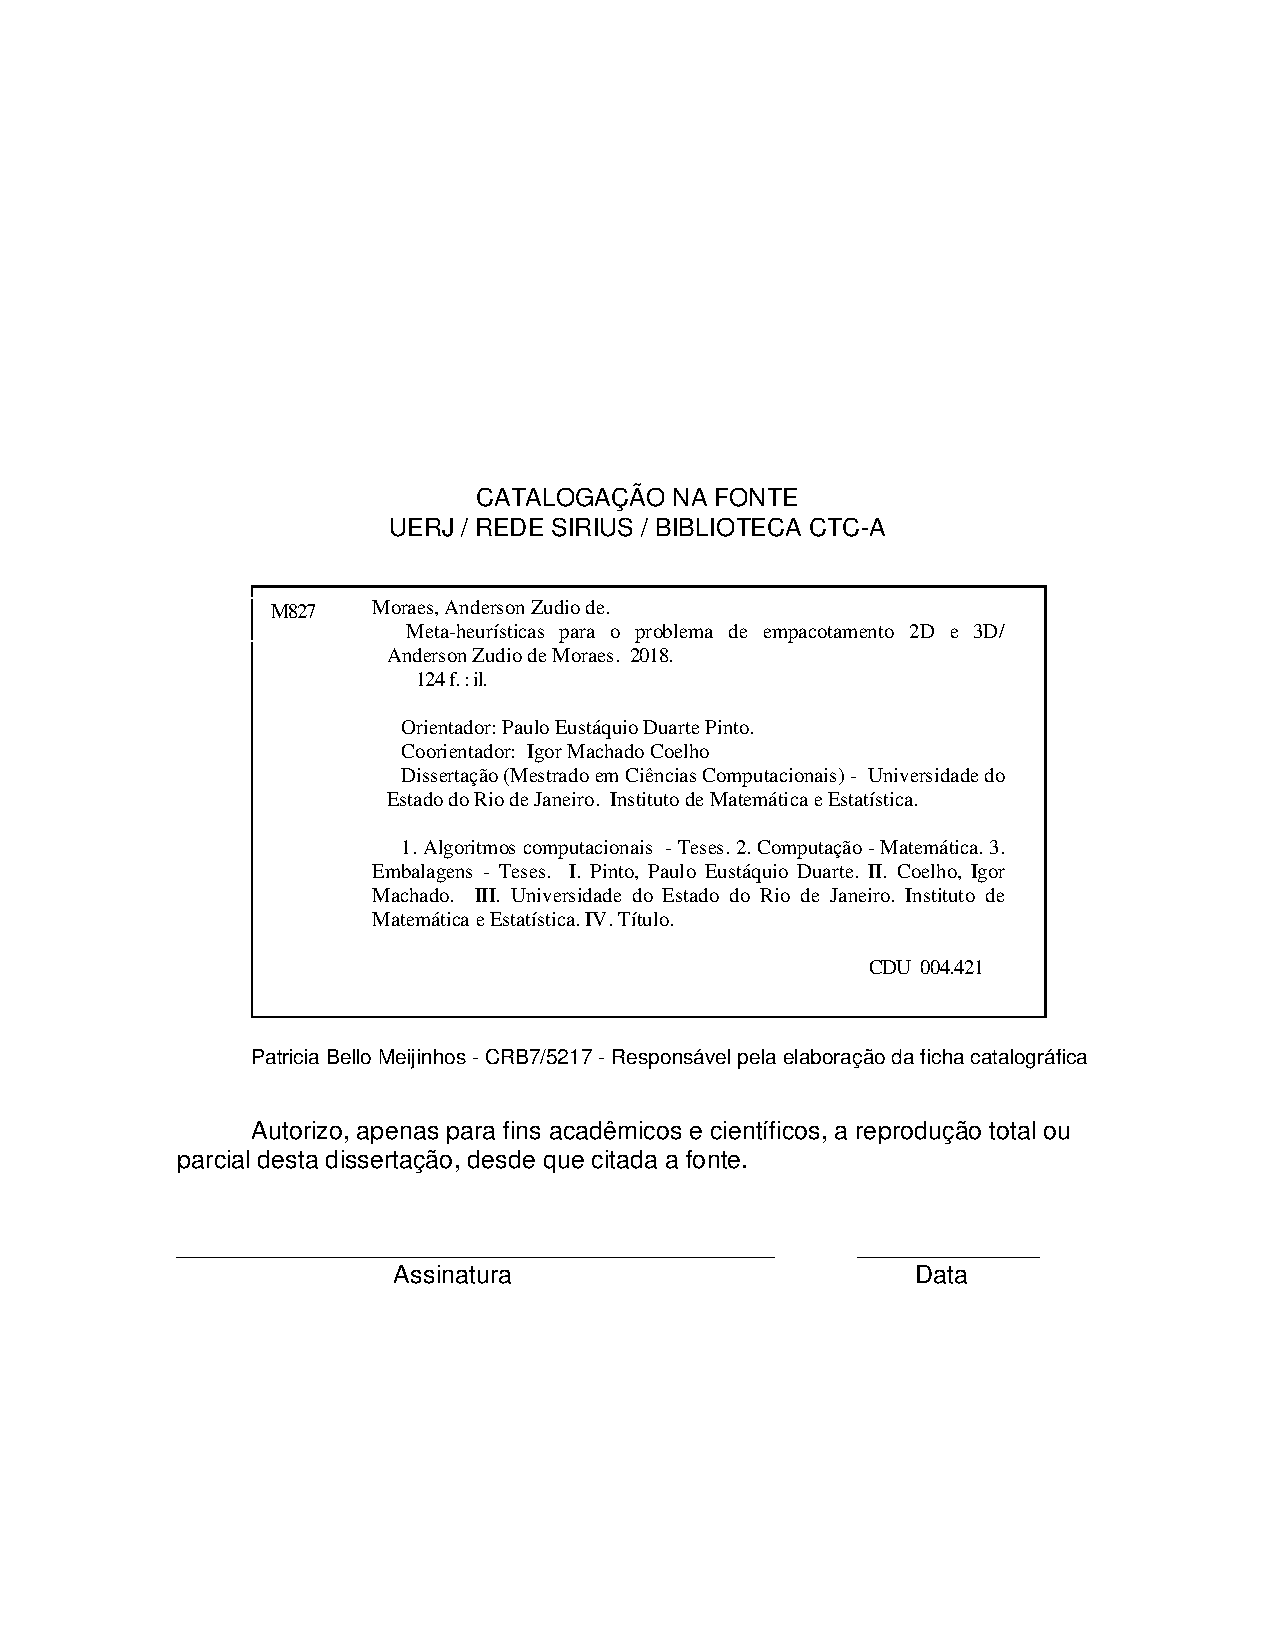
\includepdf{ficha_catalografica.pdf} %retirar até a finalização completa do trabalho  %imprimir a ficha no verso da folha de rosto!!! %pagina 3 da versao digital 

\begin{folhadeaprovacao}
    \assinatura{Prof. Dra. Cristiana Barbosa Bentes\\ Instituto de Matemática e Estatística - UERJ} %nome\\ afiliação
    \assinatura{Prof. Dr. Tiago Assumpção de Oliveira Alves\\ Instituto de Matemática e Estatística - UERJ} %nome\\ afiliação
    \assinatura{Prof. Dr. Luiz Satoru Ochi\\ Instituto de Computação - UFF} %nome\\ afiliação 
    % \assinatura{Prof. Dr. Felipe Maia Galvão França\\ Instituto Alberto Luiz Coimbra de Pós Graduação e Pesquisa de Engenharia - UFRJ} %nome\\ afiliação 
    % \assinatura{Prof. Dra. Maria Clicia Stelling de Castro\\ Instituto de Matemática e Estatística - UERJ} %nome\\ afiliação
\end{folhadeaprovacao}

%nao arrumei para o padrao uerj... formatar por conta propria seguindo roteiro
%\chapter*{Dedicatória}
%  \vfill\vfill
%    \hfill escrever,
%    
%    \hfill escrever.
%  \vfill

%\chapter*{Agradecimentos}
%  \vfill\vfill
%    \hfill escrever,
%    
%    \hfill escrever.
%  \vfill

\chapter*{\textbf{\normalsize{Agradecimentos}}}

Quero agradecer à Deus que me iluminou com as pessoas que colocou no meu caminho durante esta jornada e por toda minha vida.

Agradeço à minha esposa Izabel por todo apoio, carinho, companheirismo e amizade.

À minha mãe, pai e irmão e minha família que sempre foram os pilares na minha vida e realizações.

Aos meus orientadores, Igor e Marzulo, pelo empenho dedicado à elaboração deste trabalho e por confiarem em mim nesta empreitada.
E a todos os professores por todo o conhecimento proporcionado para minha formação e que contribuiu para este trabalho.

% ----------------------------------------------------------
% RESUMO
% ----------------------------------------------------------


\pagenumbering{gobble} %padrao da uerj -- numeracao de paginas começa na introdução -- retira numero das paginas
\renewcommand{\chaptername}{ } %padrao da biblioteca pede para esconder nome dos capitulos

\chapter*{\textbf{\normalsize\centerline{RESUMO}}}

\refbibliografica %referencia com titulo em port

Problemas de otimização são de grande importância para diversos setores da indústria, desde o planejamento de produção até escoamento e transporte dos produtos.
Diversos problemas de interesse se enquadram na classe NP-Difícil, sendo desconhecidos algoritmos eficientes para resolvê-los de forma exata em tempo polinomial.
Assim, estratégias heurísticas com capacidade de escapar de ótimos locais de baixa qualidade (meta-heurísticas) são geralmente empregadas. % FIM IGOR
A busca local é, em geral, a etapa mais custosa, em termos de tempo computacional, do processo de uma meta-heurística, desta forma torna-se muito importante fazer bom uso dos recursos nela utilizados.
Esta dissertação estuda o emprego de múltiplas estratégias de vizinhança utilizadas paralelamente para explorar um espaço de vizinhança maior e melhor aproveitar os recursos computacionais.
O processamento paralelo das estratégias de vizinhança é implementado em nível de grão fino, através de processamento em GPU, e grão grosso, por meio de processamento multi core e processamento em rede, sendo os dois níveis combinados num ambiente heterogêneo, % IGOR BEGIN
para arquiteturas von Neumann e dataflow. % IGOR END

\vspace{1em}
\noindent {Palavras-chave}: Meta-heurística, Busca Local, Dataflow, Graphics Processing Unit, Variable Neighborhood Descent.

% ----------------------------------------------------------
% Abstract
% ----------------------------------------------------------

\chapter*{\textbf{\normalsize\centerline{ABSTRACT}}}

\refbibliografic %referencia com titulo em ingles

Optimization problems have big importance in the industry field, from production management to production outflow and product transportation.
Many problems of interest are classified as NP-Hard, so there is no known algorithm to find the exact solution in a polinomial time.
Therefore heuristic strategies with the ability to escape from poor quality local optima (meta-heuristics) are generally employed.
In general, the local search is the most costly, in computational time, phase of a meta-heuristic, becoming mandatory a good use of the available resources.
The parallel processing of neighborhood strategies is implemented at the fine grain level through GPU processing and coarse grain through multi-core processing and network processing, the comibation of the two level parallelization in a heterogeneous environment for von Neumann architectures and dataflow.

\vspace{1em}
\noindent {Keywords}: Meta-heuristics, Local Search, Dataflow, Graphics Processing Unit, Variable Neighborhood Descent.

\clearpage
\listadefiguras
\clearpage
\listadetabelas
\clearpage
\listofalgorithms
\clearpage
\tableofcontents
\clearpage



%espaçamento dos demais capitulos
\titlespacing*{\chapter}{0pt}{0pt}{3cm}

\pagenumbering{arabic} %padrao da uerj -- numeracao de paginas começa na introdução -- volta numero das paginas
\setcounter{page}{12} %coloque o numero da pagina de introducao antes de mandar para a biblioteca

\chapter{Introdução}\label{cap:introducao}

Muitos dos problemas encontrados no dia-a-dia podem possuir inúmeras soluções, que em geral detêm um fator de satisfação associado (e.g.: lucro obtido, custo de utilização).
Nessa linha, o ramo da otimização atua no estudo destes de modo a buscar minimizar ou maximizar o valor da função objetivo (satisfação) associada.

Conforme pode ser visto na Figura~\ref{fig:espacoDeBusca}, um método de otimização explora o espaço de busca a procura da solução que apresente o melhor valor de função objetivo.

\begin{figure}[htpb]
    \centering
    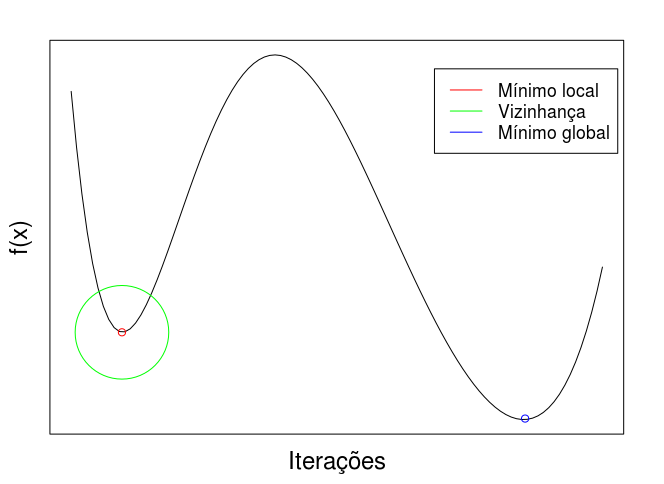
\includegraphics[scale=0.6]{figuras/desenharCurva-semEixo.png}
    \caption{Espaço de busca explorado por um método de otimização. São indicados mínimo local, mínimo global e vizinhança, conceitos que serão definidos a frente.}
    \label{fig:espacoDeBusca}
\end{figure}

Quando é necessário resolver problemas de otimização, um campo promissor é o das meta-heurísticas, contudo estes algoritmos podem demandar muito tempo de processamento, especialmente ao se resolver problemas com grandes instâncias. Isto posto, podemos ressaltar a importância de utilizar métodos eficientes para resolução de tais problemas.

Uma parte importante no universo das meta-heurísticas são os algoritmos de busca que, inicialmente, recebem uma solução para um problema e rastreiam seu espaço de busca para então retornar a melhor solução encontrada.
O espaço de busca é um super conjunto de algumas estratégias de vizinhança para a solução atual e as que surgirem.

Uma boa alternativa para melhorar o tempo de processamento destes problemas é pela utilização de programação paralela~\cite{handbookmeta}.
A maioria dos algoritmos de otimização até então projetados foram feitos para funcionarem de forma ``naturalmente'' sequencial, criando uma árdua tarefa, muitas vezes hercúlea, para os programadores que desejam alterar a implementação do algoritmo para rodar de forma paralela.
A abordagem mais utilizada para paralelização de meta-heurísticas consiste em escolher métodos ou partes do método que podem ser executadas independentemente e lançar sua execução paralela (\emph{Bag-of-Tasks}).
Não obstante apenas alguns trabalhos científicos são dedicados a realmente re-projetar estes algoritmos para aproveitar o poder de arquiteturas paralelas de forma profunda~\cite{vns2015, jpdc2017, endm2018:araujo}.

% Sugestão [MARZULO]
Em abordagens tradicionais para paralelização de aplicações são empregadas arquiteturas \emph{Multiple Instruction Multiple Data} (\emph{MIMD})~\cite{flynn1972}, onde cada elemento de processamento possui \emph{streams} de instruções e dados independentes.
Desta forma, o desenvolvedor pode particionar as tarefas de sua aplicação para que sejam executadas em \emph{threads} ou processos, mapeadas nos elementos de processamento.
A comunicação entre tarefas pode ser realizada por memória compartilhada (multiprocessadores ou \emph{multicores}) ou por troca de mensagens (como em \emph{clusters} de computadores).
% A abordagem mais direta de paralelizar uma aplicação é usando múltiplas threads ou processos numa máquina com múltiplos processadores (ou múltiplos cores) ou utilizando muitos computadores (e.g., um cluster de máquinas), i.e. usando uma arquitetura Multiple Instruction Multiple Data (MIMD)~\cite{flynn1972}.
Estes processadores seguem o modelo de Von Neumann, no qual a execução de uma instrução é guiada pelo fluxo de controle, de forma que a ordem das instruções no programa prescreve o que o processador deve fazer passo a passo.
Este modelo assume que um \textit{program counter} é usado para indicar a próxima instrução a ser executada e estas podem alterar o estado da máquina ao alterar valores de uma estrutura de armazenamento global, como um banco de registradores, cache ou memória principal.

Trabalhos recentes em modelos e linguagens de programação paralela~\cite{trebuchetijhpsa,1473,1136512,Gupta:2011:DES:2155620.2155628,tbbflow,journals/pc/BosilcaBDHLD12,Giorgi2014} geraram novos \emph{frameworks} para o modelo de programação dataflow, em diferentes níveis de abstração e granularidade, como solução para representar programas considerando as operações como ponto de vista principal, permitindo assim uma modelagem mais fácil de muitos problemas ao alta performance.
Está claro que em alguns casos o esforço de programação (medido em termos de tempo de programação ou linhas de código) é consideravelmente reduzido quando se utiliza programação dataflow para paralelizar as aplicações, se compararmos com as ferramentas tradicionais como OpenMP ou Pthreads.
Além disso, o desempenho da execução do aplicações desenvolvidas conforme o modelo dataflow pode ser comparado com métodos tradicionais \cite{trebuchetijhpsa,lcswamca}.
% Teve um revisor que contestou esse "de fato", mantenho isso? 
% Corroborando assim dataflow como uma técnica \textit{de facto} para programação paralela, de forma que oferece facilidade de programação e boa performance.

A Figura~\ref{fig:dataflowExemplo} mostra um paralelo entre a versão Von Neumann, no quadro A e a implementação do mesmo código no modelo dataflow, exemplificada no quadro B.
Pelo quadro B pode-se perceber que a execução das operações $x + y$ e $k * j$ podem ser executadas em qualquer ordem, ou mesmo simultaneamente, sem alterar o resultado final da execução.

\begin{figure}[htpb]
    \centering
    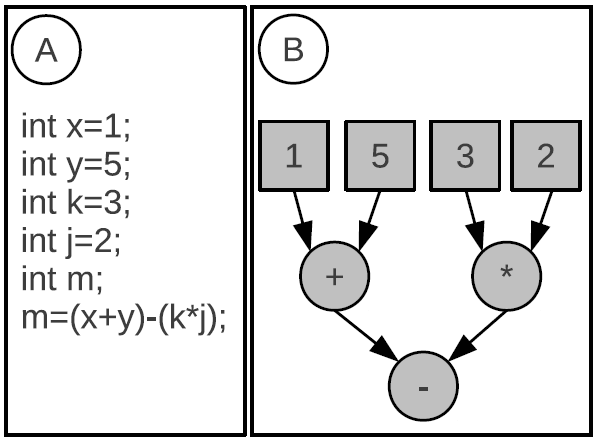
\includegraphics[scale=0.6]{figuras/dataflow/dataflowExemplo.png}
    \caption{Exemplo de conversão código para grafo de dependências, conforme apresentado em~\cite{teseMarzulo}.
    O quadro A mostra um trecho de código e o quadro B o grafo dataflow associado.}
    \label{fig:dataflowExemplo}
\end{figure}

Usualmente a programação dataflow é feita instanciando trechos de código e os conectando em um grafo de acordo com suas dependências de dados, livrando assim o programador de grande parte da complexidade da programação paralela uma vez que esta, bem como a sincronização, são realizados pelo ambiente de execução dataflow.
O modelo dataflow expõe naturalmente o paralelismo, instruções são executadas conforme suas dependências de dados (na ordem do fluxo de dados, dataflow), i.e., instruções são disparadas assim que seus operandos estão disponíveis, dessa forma o desafio passa a ser modelar o grafo de dependências das operações tendo como uma importante decisão a se tomar o tamanho do grão de cada nó do grafo de forma a comportar o paralelismo sem sobrecarregar o algoritmo podendo assim causar um \emph{overhead} desnecessário na troca de mensagens.

Problemas NP-Difíceis~\cite{GareyJohnson1990} surgem de cenários práticos, como o roteamento de um conjunto de veículos para entregas e coletas, ou visitar um conjunto de cidades percorrendo a menor rota possível.
Este último sendo conhecido como Problema do Caixeiro Viajante (PCV), um dos mais importantes (e não resolvidos) problemas no campo da ciência da computação.
Devido a sua combinatoriedade natural, não existe algoritmo conhecido que resolva o PCV em tempo polinomial.
Todavia, muitos algoritmos heurísticos e combinações de métodos exatos com métodos heurísticos são capazes de resolver o PCV para instâncias com milhares de cidades.
Como uma variante menos explorada do PCV, consideramos o Problema da Mínima Latência (PML), que é uma variante do PCV onde todos os nós precisam ser visitados, mas o custo é o somatório do acumulado das distâncias ponto a ponto.

Muitos trabalhos recentes produziram algoritmos que obtiveram resultados eficientes utilizando RVND~\cite{souza2010, silva2012,subramanian2013}, cuja ideia principal é que ao se atingir um mínimo local para uma estratégia de vizinhança ainda pode existir um vizinho em outra vizinhança com valor de função objetivo melhor que o já encontrado, o que motivou a implementação de uma versão distribuída.
O DVND, proposto em~\cite{RIOS201839}, é uma versão paralela do método de busca VND, adotando-se uma visão dataflow para o algoritmo é possível uma implementação conforme a encontrada em \cite{df-dvnd2018}.
A arquitetura multi-core do DVND torna possível explorar diferentes vizinhanças simultaneamente (com diferentes implementações de busca local), e escolher o melhor resultado dos métodos de busca.
Não obstante, os autores que obtiveram o estado da arte nos resultados para o PML não chegaram a estender a implementação do DVND para múltiplos e independentes nós de processamento devido a problemas de performance, serialização de dados e controle de fluxo utilizando a tecnologia MPI~\cite{jpdc2017}.
Por esse motivo esse trabalho propõe uma nova implementação do DVND capaz de lidar com múltiplos nodos de maneira mais natural, modelando o método como um grafo dataflow e usando o framework em Python para dataflow Sucuri~\cite{sucuri-original}.

% Comentei isso porque achei que ficou meio descontextualizado
%Entretanto, no mundo real, os problemas tendem a ser inter relacionados uns aos outros e resolver separadamente as subpartes do problema não necessariamente resolve o problema em si. Este é o caso em vários aplicações práticas de problemas clássicos como o Problema da Mochila ~\cite{Pisinger:1995} e o Problema do Caixeiro Viajante~\cite{Dantzig:1954}. Muitas outras variantes desses problemas clássicos podem ser encontradas na literatura, contudo poucos são bem sucedidos ao combinar os problemas de forma a desaviar os algoritmos no estado da arte atual.

%In this paper we deal with the Traveling Thief Problem (TTP) \cite{Bonyadi:2013}, a combination of the Traveling Salesman Problem (TSP) and the 0/1 Knapsack Problem (KP), using both classic well known optimization problems.
% Preciso citar isso?
%These two components have been merged in such a way that the optimal solutions for each problem do not necessarily correspond to an optimal TTP solution~\cite{wagner:2017}.
%A practical application for the TTP is indicated by Mei et al.~\cite{mei:2015} and consists of a routing problem with service profit, where each costumer has a demand and a service profit, and the travel cost depends on the load of the vehicle.
%Another evidence for the importance of considering the impact of vehicle load in travel costs is related to carbon emissions and can be seen in the Green Vehicle Routing Problem literature~\cite{Lin:2014}.
%By studying the TTP it is possible to perform a systematic investigation of interactions between two hard optimization problems, to eventually help solving real-word problems more efficiently~\cite{Bonyadi:2016}.

\section{Motivação}\label{sec:motivacao}

Inúmeras aplicações práticas podem utilizar meta-heurísticas para resolver problemas de otimização, sendo comum para muitos desses processos sua etapa final ser constituída de um algoritmo de busca local.
Este por sua vez faz uso de estratégias de vizinhança para enumerar o espaço de busca.
% (e.g. Swap, 2-Opt, OrOpt-2, ..., etc)
Versões clássicas do processos de busca local utilizam uma vizinhança em conjunto com uma estratégia de exploração (Primeira melhora, Melhor vizinho).

% Cito o VND ao mencioná-lo aqui?
Poucos são os trabalhos da literatura que combinam estratégias de vizinhança diferentes como em \emph{Variable Neighborhood Descent} (\emph{VND}) e mais raros são os trabalhos que usam diferentes estratégias de exploração de vizinhança como em \cite{vns2015}.

\section{Objetivos} \label{sec:objetivos}

% Emprego de múltiplas estratégias de vizinhança com uso de GPU para solução de problemas de otimização
Este estudo visa propor estratégias diferenciadas de solução de problemas de otimização, para tanto podemos enumerar os seguintes objetivos:
\begin{itemize}
    \item{A investigação do uso de estratégias distintas de vizinhanças almeja a realização de uma busca mais extensa no espaço de soluções, contudo isto aumenta sua complexidade computacional, o que abre caminho para o item seguinte;}
    \item{Propor algoritmos paralelos que se beneficiam de tecnologias emergentes, porém ainda pouco exploradas no ramo da pesquisa operacional, que é a utilização de aceleração pelo uso de placas gráficas;}
    \item{Utilizar melhor os recursos usados no processamento realizado ao aproveitar computações realizadas em nós diferentes.}
\end{itemize}

O objetivo final é propor um método que seja capaz de fazer uso de múltiplas estratégias de vizinhança aproveitando recursos de paralelização de grão fino e grão grosso sem precisar acoplar a solução a um problema específico.

\section{Estrutura deste documento}\label{sec:estrutura}

O restante deste trabalho é organizado conforme o segue:

\begin{itemize}
    \item Capítulo~\ref{cap:conceitos}: descreve os fundamentos teóricos e termos utilizados nessa dissertação, no desenvolvimento deste capítulo são caracterizados e ilustrados os termos e meta-heurísticas utilizados por descrições independentes;
    \item Capítulo~\ref{cap:metodologia}: descreve e apresenta os algoritmos propostos para resolver o Problema da Mínima Latência mas não se limitando a este problema. Este capítulo detalha os métodos bem como seus componentes e pseudocódigos;
    \item Capítulo~\ref{cap:resultados}: mostra os resultados computacionais deste trabalho. Os métodos Dataflow DVND e GDVND propostos podem utilizar diferentes estratégias e da mesma forma podem ser aplicados a problemas variados;
    \item Capítulo~\ref{cap:conclusao}: apresenta as conclusões do trabalho desenvolvido nessa dissertação com as propostas de trabalhos futuros.
\end{itemize}
 %introducao nao conta como capitulo
\chapter{Revisão de literatura e conceituação teórica} \label{cap:conceitos}

Este capítulo tem como objetivo introduzir os conceitos teóricos básicos utilizados no documento e bases para apresentar a método.

\section{Problemas de Decisão} \label{sec:problemaDecisao}

Um problema $\Pi$ é dito um problema de decisão quando seu conjunto solução é composto apenas pelos elementos \textit{Sim} e \textit{Não}, ou seja:
\begin{equation} \label{eq:problemaDecisao}
\begin{split}
\Pi: D \rightarrow Im  \\
Im = \{ Sim, N\widetilde{a}o \}
\end{split}
\end{equation}

São exemplos de problemas de decisão:
\begin{itemize}
    \item{Seja $x \in C$, sendo $x$ um número pertencente ao conjunto $C$, $x$ é o menor número deste conjunto?}
    \item{Seja um grafo $G(V,A)$ denotado pelos arestas $A$ e vértices $V$, existe um caminho do vértice $x$ para o vértice $y$ com custo menor que $c$?}
\end{itemize}

\section{Problemas de Otimização} \label{sec:problemaOtimizacao}

Seja $\Pi$ um problema, S o conjunto de soluções viáveis para o mesmo e $f$ a função objetivo que associa uma solução $s_i$ a um valor numérico então temos:
\begin{equation}  \label{eq:problemaOtimizacao}
\begin{split}
S = \{s_1, s_2, \dots, s_n \} \\
f: S \rightarrow \mathbb{R}
\end{split}
\end{equation}

Um problema de otimização, em geral, pode ser de minimização ou de maximização.
$\Pi$ é um problema de minimização se ele consiste em determinar uma solução $s^*$ tal que:
\begin{equation}  \label{eq:problemaOtimizacaoMinimizar}
s^* \in S \mid f(s^*) \leq f(s), \forall s \in S
\end{equation}

De forma análoga um problema de minimização pode ser dado por:
\begin{equation}  \label{eq:problemaOtimizacaoMaximizar}
s^* \in S \mid f(s^*) \geq f(s), \forall s \in S
\end{equation}

Os problemas de otimização podem ser divididos em dois tipos:

\begin{itemize}
    \item Otimização contínua: nesse tipo de problema pelo menos uma das variáveis $x$ do conjunto de variáveis $X$ pode assumir infinitos valores;
    \item Otimização combinatória: problemas em que toda variável $x$ no conjunto de variáveis $X$ é discreta, podendo assumir apenas um número finito ou infinito porém contável de valores.
\end{itemize}

Desta forma, existe um número finito de soluções viáveis para um problema de otimização combinatória.
Para todo problema de decisão existe um problema de otimização associado, tomemos com exemplo os problemas da seção~\ref{sec:problemaDecisao} e teremos os seguintes problemas de otimização:

\begin{itemize}
    \item Seja um conjunto $C$, encontrar $x \in C \mid x < y, \forall y \in C$.
    \item Seja um grafo $G(V,A)$ denotado pelos arestas $A$ e vértices $V$, encontrar o menor caminho do vértice $x$ para o vértice $y$.
\end{itemize}

\section{Problema da Mínima Latência}\label{sec:mlp}

O Problema da Mínima Latência (PML) é um problema de otimização, sendo uma variante do PCV no qual o objetivo é minimizar o tempo de chegada (ou latência) aos vértices, e não a distância ou tempo da rota como no problema original.
O PML pode ser definido como um grafo direcionado $G=(V,E)$, onde $V=\{0,1,\dots,n\}$ é um conjunto de vértices e $E = \{(i, j) : i, j \in V, i \ne j \}$ um conjunto de arestas que conectam os vértices.
Para cada arco $(i,j)$ existe um tempo de viagem associado igual a $t(i,j)$. O vértice 0 representa o ponto de saída (depósito) e os demais os clientes a serem visitados.
O tempo de chegada (ou latência) a um cliente $i \in V$, é denotado por $l(i)$, o qual é definido pelo tempo de viagem do depósito até o vértice $i$.

\begin{figure}[htpb]
    \centering
    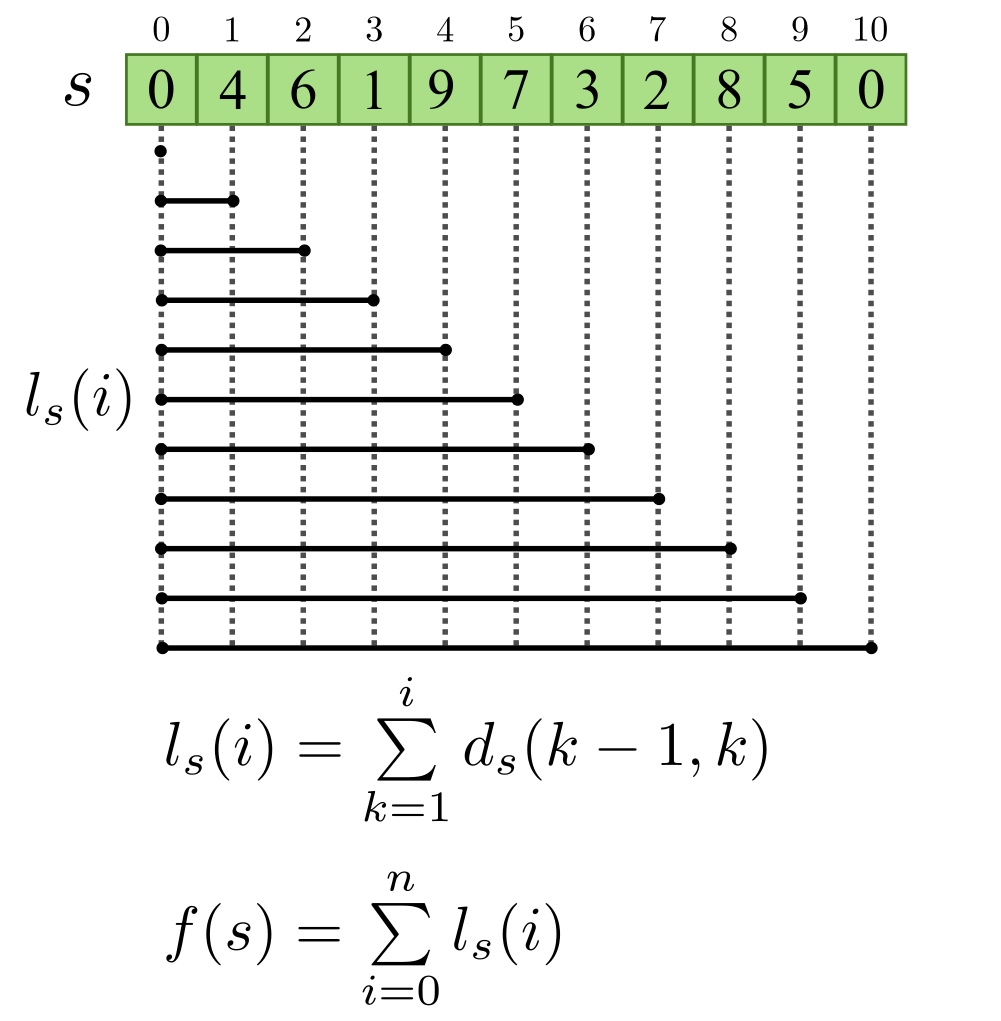
\includegraphics[width=0.6\linewidth]{figuras/pml/mlp}
    \caption{Exemplo de solução com as latências de cada cidade e cálculo da função objetivo}
    \label{fig:pmlDiagramaFormulas}
\end{figure}

O objetivo do PML é, iniciando do depósito, determinar o ciclo Hamiltoniano $s$ que minimize a latência expressa por $L(s)=\sum_{i=0}^{n} l(i)$ como pode ser visto na Figura~\ref{fig:pmlDiagramaFormulas}.
Assim sendo, uma solução viável do PML consiste numa permutação de $n$ clientes determinando a ordem de visita dos mesmos. Tomemos o exemplo a seguir, se $n=9$,  $s=[0,8,3,7,1,4,2,5,6,0]$ é uma solução viável para o PML (de fato, qualquer permutação $1..8$ começando e terminando no vértice zero é uma solução viável).

Apesar da formulação simples e de sua grande aplicação na otimização de latência em redes, o PML é um problema complexo, sendo provado que o PML é NP-Difícil~\cite{silva2012}. A despeito da semelhança na formulação do PML com a do Problema do Caixeiro Viajente (PCV) a sua função objetivo é mais complexa de ser calculada que a do PCV.
No PML, pequenas alterações no vetor solução podem levar a grandes alterações no resultado final da solução e a natureza não local da função objetivo faz com que uma simples inserção afete todas as latências subsequentes.
Na literatura, o PML também é conhecido Problema do Caixeiro Viajante Cumulativo \cite{bianco1993}, Problema do Entregador \cite{mladenovic2013} e Problema do Reparador Viajante. \cite{tsitsiklis1992}.

Em trabalhos recentes, um procedimento de busca local baseado em \emph{Graphics Processing Unit} (\emph{GPU}) e computação \emph{multi-core} foi proposto para o PML~\cite{wamca2016}.
A ideia foi chamada \emph{Distributed Variable Neighborhood Descent} (\emph{DVND}), tentando explorar diferentes estratégias de vizinhança simultaneamente para uma solução de entrada.

Em otimização, uma vizinhança é definida como um conjunto de operações chamados "movimentos", que são capazes de realizar pequenas alterações na solução de entrada.
Estas alterações podem ser, por exemplo, trocar dois elemento na permutação inicial, gerando dessa forma $\mathcal{O}(N^2)$ diferentes soluções (para o caso de uma permutação de tamanho $N$). Existe na literatura muitas dessas vizinhanças (como 2-Opt, OrOpt-1, OrOpt-2, Swap, ..., etc), conquanto por limitações computacionais estes são sempre explorados de forma sequencial, chamados de \emph{Variable Neighborhood Descent} (\emph{VND}).
Com o objetivo de encontrar um ótimo local para o PML, a ideia principal do DVND é usar GPU para obter operações de grão fino (que em geral são rápidas) e explorar toda a vizinhança $\mathcal{O}(N^2)$ mais rápido que em CPU (como explicado em~\cite{wamca2016}) e combinar as respostas das buscas, escolhendo a nova melhor solução.

% \subsection{Exemplo}

% \begin{figure}[htpb]
%     \centering
%     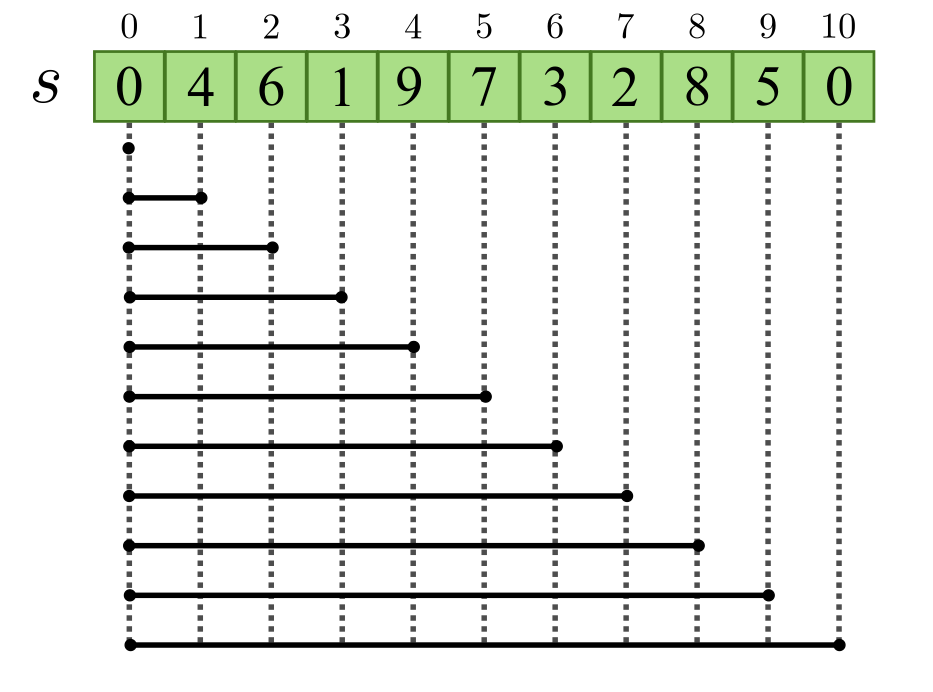
\includegraphics[width=0.6\linewidth]{figuras/pml/mlp-clean}
%     \caption{Exemplo de solução com as latências de cada cidade}
%     \label{fig:pml}
% \end{figure}

Pelo exemplo na Figura~\ref{fig:pmlDiagramaFormulas} podemos ver que o valor da latência $L(s)$ será dado palos somatórios das latências de todas as cidades, sendo $d_s^{i, j}$ a distância da cidade $i$ para a cidade $j$ na solução $s$, então temos:
$$ L(s) = \sum_{i=0}^n{l_s(i)} $$
$$ L(s) = l_s(0) + l_s(1) + l_s(2) + l_s(3) + l_s(4) + l_s(5) + l_s(6) + l_s(7) + l_s(8) + l_s(9) $$
$$ L(s) = 10d_s^{0, 4} + 9d_s^{4, 6} + 8d_s^{6, 1} + 7d_s^{1, 9} + 6d_s^{9, 7} + 5d_s^{7, 3} + 4d_s^{3, 2} + 3d_s^{2, 8} + 2d_s^{8, 5} + d_s^{5, 0}$$

\section{Busca local} \label{sec:buscaLocal}

Um algoritmo de busca local percorre iterativamente o espaço de soluções de um determinado problema melhorando a solução atual.
Para tanto procura na vizinhança (definida na Seção~\ref{subsec:vizinhanca}) atual por uma solução melhor que a atual e repete o processo até não ser encontrada uma melhora.

\subsection{Vizinhança} \label{subsec:vizinhanca}

Seja $S$ o espaço de soluções de um problema de otimização $\Pi$, e $s \in S$ uma solução qualquer, considere a função objetivo $f: S \rightarrow \mathbb{R}$ que atribui um valor para cada solução.
Denotamos então por $N^x(s)$ o conjunto de soluções vizinhas de $s$ para a vizinhança $x$ com $N^x(s) \subseteq S$, em que as soluções dessa vizinhança podem ser obtidas de $s$ a partir da aplicação de determinadas operações.
Uma solução $s'$ é vizinha de $s$ (isto é $s' \in N^x(s)$) segundo uma vizinhança $s$ se $s'$ é alcançável a partir de $s$ fazendo uso de uma pequena perturbação nesta última.

\subsection{Movimento} \label{subsec:movimento}

% Seja $S$ o espaço de soluções de um problema de otimização $\Pi$, e $s \in S$ uma solução qualquer, considere a função objetivo $f: S \rightarrow \mathbb{R}$ que atribui um valor para cada solução.
Considere $m^k: S \rightarrow S$ a função que representa um movimento que leva uma solução $s$ a uma solução $s'$ ou de forma equivalente $s' = m^k \circ s$.
Designamos então o movimento $m^k \in M^k$ no conjunto de movimentos da vizinhança $k$.

Adicionalmente podemo definir o custo do movimento $m^k(s)$ em relação a solução $s$ como sendo a diferença entre o valor da solução $s'$ gerada ao aplicar este movimento à solução $s$ e o valor da solução $s$, conforme pode ser visto na Equação~\ref{eq:movimentoCusto}, iremos omitir a função $f$ e a vizinhança $k$ quando estiverem claros no contexto, desta forma a podemmos simplificar a notação conforme a Equação~\ref{eq:movimentoCustoSimplificada}.
Formalmente, a notação circunflexo representa a função $\widehat{m}: S \rightarrow \mathbb{R}$.
\begin{equation} \label{eq:movimentoCusto}
\widehat{m^k_f}(s) = f(s') - f(s)
\end{equation}

\begin{equation} \label{eq:movimentoCustoSimplificada}
\widehat{m^k_f}(s) = \widehat{m}(s) = f(s') - f(s)
\end{equation}

Para exemplificar as definições que se seguem tomemos a Tabela~\ref{tab:coordenadasComMatrizDistancias}, consideremos um conjunto de cidades com suas localizações conforme a Tabela~\ref{tab:coordenadasCidades}.
Para facilitar o acompanhamento considere a matriz de distâncias expressa na Tabela~\ref{tab:distanceMatrix}.

\begin{table}[ht]
    \centering
    \begin{subtable}{.3\textwidth}
    \centering
    \begin{tabular}{c|cc}
    	\hline
    	Cidade & $x$ & $y$ \\
    	\hline
    	A &	200 &	200 \\
    	B &	100 &	400 \\
    	C &	200 &	800 \\
    	D &	400 &	900 \\
    	E &	600 &	700 \\
    	F &	900 &	600 \\
    	G &	1000 &	400 \\
    	H &	700 &	100 \\
    	I &	500 &	200 \\
    	\hline
    \end{tabular}
    \caption{Coordenadas das cidades.}
    \label{tab:coordenadasCidades}
    \end{subtable}% <---- don't forget this %
    \begin{subtable}{.675\textwidth}
    \centering
    \begin{tabular}{c|ccccccccc}
    	\hline
    	   &   A&   B&   C&   D&   E&   F&   G&   H&   I\\
    	\hline
    	 A &    & 224& 600& 728& 640& 806& 825& 510& 300\\
    	 B & 224&    & 412& 583& 583& 825& 900& 671& 447\\
    	 C & 600& 412&    & 224& 412& 728& 894& 860& 671\\
    	 D & 728& 583& 224&    & 283& 583& 781& 854& 707\\
    	 E & 640& 583& 412& 283&    & 316& 500& 608& 510\\
    	 F & 806& 825& 728& 583& 316&    & 224& 539& 566\\
    	 G & 825& 900& 894& 781& 500& 224&    & 424& 539\\
    	 H & 510& 671& 860& 854& 608& 539& 424&    & 224\\
    	 I & 300& 447& 671& 707& 510& 566& 539& 224& \\
    	 \hline
    \end{tabular}
    \caption{Matriz de distâncias euclidianas com valores inteiros arredondados.}
	\label{tab:distanceMatrix}
    \end{subtable}
\caption{Informações de distâncias e localização das cidades para os exemplos apresentados.}
\label{tab:coordenadasComMatrizDistancias}
\end{table}

Tomemos como exemplo a solução $s_1$ expressa na Figura~\ref{fig:figuraExemplo_s1}, este apresenta uma solução para o problema apresentado na Tabela~\ref{tab:coordenadasComMatrizDistancias} com valor de função objetivo 2631 para o PCV e 13074 para o PML.

\begin{figure}[ht]
    \begin{minipage}{.475\textwidth}
        \begin{subfigure}[t]{1\textwidth} %
            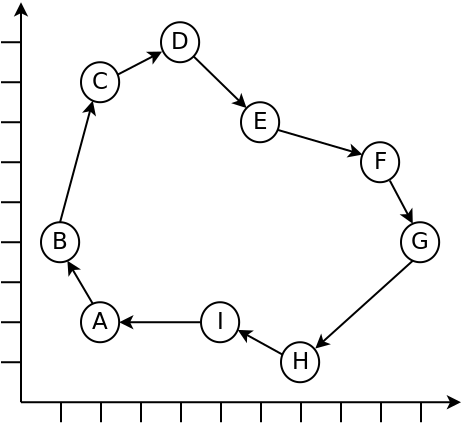
\includegraphics[width=1\linewidth]{figuras/pml/exemplo-rodolfo-opt.png}
        \end{subfigure}
    \end{minipage}
    \begin{minipage}{.475\textwidth}
\begin{Verbatim}[commandchars=\\\{\}]
index:   0  1  2  3  4  5  6  7  8
cidade:  A  B  C  D  E  F  G  H  I
\end{Verbatim}
\begin{gather*}
    f(s_1): 2631/13074 \ (PCV/PML)
\end{gather*}
    \end{minipage}
    \caption{Solução $s_1$.}
    \label{fig:figuraExemplo_s1}
\end{figure}

Ao aplicarmos à solução anterior $s_1$ o movimento $m_1$ 2-opt(1,7), exibido na Figura~\ref{fig:figuraExemplo_m1s1}, este reverte bloco de 1 a 7 (remove implicitamente duas arestas e reconecta a rota), o custo do movimento é $\widehat{m_1}(s_1)$: 509 para o PCV e 3113 para o PML.

\begin{figure}[ht]
    \begin{minipage}{.475\textwidth}
        \begin{subfigure}[t]{1\textwidth} %
            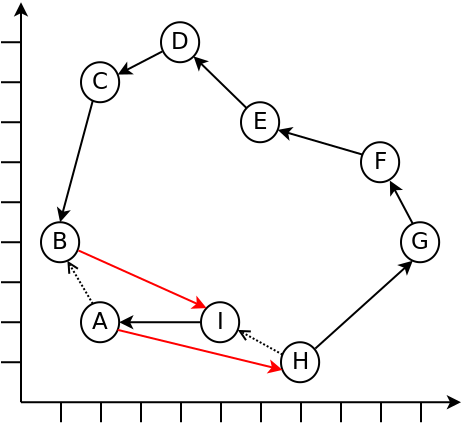
\includegraphics[width=1\linewidth]{figuras/pml/exemplo-rodolfo-2opt-1-7.png}
        \end{subfigure}
    \end{minipage}
    \begin{minipage}{.475\textwidth}
\begin{Verbatim}[commandchars=\\\{\}]
index:  0  1  2  3  4  5  6  7  8
cidade: A  \textcolor{red}{H  G  F  E  D  C  B}  I
\end{Verbatim}
\begin{gather*}
f(m_1 \circ s_1) = 3140/16187 \ (PCV/PML) \\ 
\widehat{m_1}(s_1)+f(s_1) = \\ 
509 + 2631 = 3140 \ (PCV)\\
3113 + 13074 = 16187 \ (PML)
\end{gather*}
    \end{minipage}
    \caption{Solução $m_1 \circ s_1$, com $m_1$ sendo 2-opt(1,7).}
    \label{fig:figuraExemplo_m1s1}
\end{figure}

Outra opção seria escolher o movimento $m_2$ 2-opt(5,6) para ser aplicado à solução, este reverte bloco de 5 a 6 (remove implicitamente duas arestas e reconecta rota), neste caso o custo do movimento é $\widehat{m_2}(s_1)$: 299/1265 para o PCV e PML respectivamente, em detalhes na Figura~\ref{fig:figuraExemplo_m2s1}.

\begin{figure}[ht]
    \begin{minipage}{.475\textwidth}
        \begin{subfigure}[t]{1\textwidth} %
            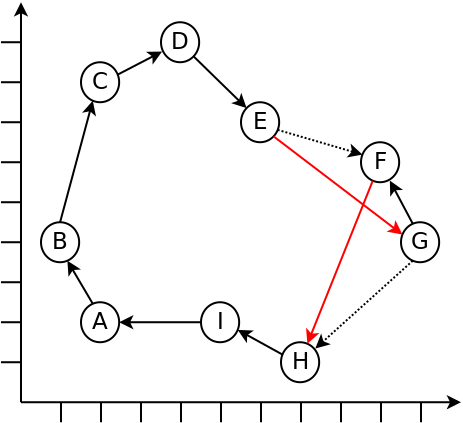
\includegraphics[width=1\linewidth]{figuras/pml/exemplo-rodolfo-2opt-5-6.png}
        \end{subfigure}
    \end{minipage}
    \begin{minipage}{.475\textwidth}
\begin{Verbatim}[commandchars=\\\{\}]
index:   0  1  2  3  4  5  6  7  8
cidade:  A  B  C  D  E  \textcolor{blue}{G  F}  H  I
\end{Verbatim}
\begin{gather*}
f(m_2 \circ s_1): 2930/14339 \ (PCV/PML) \\
\widehat{m_2}(s_1)+f(s_1) = \\
299 + 2631 = 2930 \ (PCV) \\
1265 + 13074 = 14339 \ (PML)
\end{gather*}
    \end{minipage}
    \caption{Solução $m_2 \circ s_1$, com $m_2$ sendo 2-opt(5,6).}
    \label{fig:figuraExemplo_m2s1}
\end{figure}

Adicionalmente se pode ver que a Figura~\ref{fig:figuraExemplo_m3s1} mostra o movimento $m_3$ 2-opt(1,3) sendo aplicado à solução $s_1$, este reverte bloco de 1 a 3 (remove implicitamente duas arestas e reconecta rota) e apresenta um custo de $\widehat{m_3}(s_1)$: 804/6148 para o PCV e PML.

\begin{figure}[ht]
    \begin{minipage}{.475\textwidth}
        \begin{subfigure}[t]{1\textwidth} %
            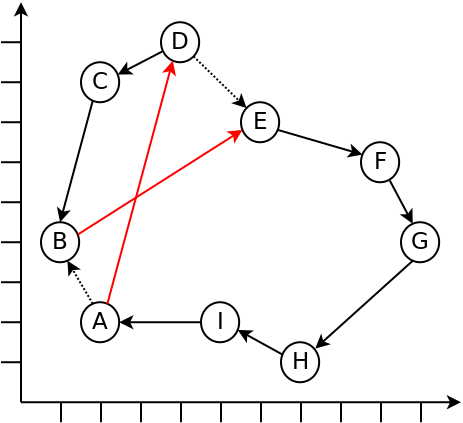
\includegraphics[width=1\linewidth]{figuras/pml/exemplo-rodolfo-2opt-1-3.png}
        \end{subfigure}
    \end{minipage}
    \begin{minipage}{.475\textwidth}
\begin{Verbatim}[commandchars=\\\{\}]
index:   0  1  2  3  4  5  6  7  8
cidade:  A  \textcolor{green}{D  C  B}  E  F  G  H  I
\end{Verbatim}
\begin{gather*}
f(m_3 \circ s_1): 3435/19222 \ (PCV/PML) \\
\widehat{m_3}(s_1)+f(s_1) = \\
804 + 2631 = 3435 \ (PCV)\\
6148 + 13074 = 19222 \ (PML)
\end{gather*}
    \end{minipage}
    \caption{Solução $m_3 \circ s_1$, com $m_3$ sendo 2-opt(1,3).}
    \label{fig:figuraExemplo_m3s1}
\end{figure}

\subsubsection{Movimentos livres de estrutura -- \emph{structure-free moves}} \label{subsubsec:movimentosLivresDeContexto}

Quando a estrutura de armazenamento interna utilizada para representar uma solução permite a aplicação de um movimento para qualquer solução temos um movimento livre de estrutura.
Em outras palavras, um movimento $m$ é livre de estrutura se ele sempre pode ser aplicado a uma solução $s$ sem gerar uma solução inválida.

\begin{equation} \label{eq:movimentoLivreDeContexto}
m \ \textrm{é livre de estrutura} \  \iff m \circ s \in S, \forall s \in S
\end{equation}

Quando uma classe de movimentos é livre de estrutura para um determinado problema então se pode dizer que a função a representar este movimento é fechada para o conjunto de soluções $S$.

A caracterização de um movimento como livre de estrutura depende de suas restrições e da sua representação.
Desta forma, para o Problema do Caixeiro Viajante em que o grafo com as distâncias entre as cidades é completo, o movimento \textit{Swap} será livre de estrutura contudo num grafo incompleto uma aplicação do \textit{Swap} pode gerar uma solução inviável pois pode não existir um determinado percurso após a alteração na solução.

\subsubsection{Movimentos fracamente independentes -- \emph{weakly independent moves}} \label{subsubsec:movimentosParcialmenteIndependentes}

Dois movimentos $\{m_2,m_3\} \subseteq \mathcal{I}$ são fracamente independentes quando a aplicação de um deles não altera o custo do outro movimento para apenas um dos movimentos.
Formalmente temos que dois movimentos $m_1$ e $m_2$ são parcialmente independentes, ou seja $m_1 \parallel_p m_2$, se e somente se:
\begin{equation}
% \begin{align}
m_1 \parallel_p m_2 \iff \widehat{m_1}(s) = \widehat{m_1}(m_2 \circ s)
\label{eq:movimentosParcialmenteIndependentes}
% \end{align}
\end{equation}

\begin{corolario}
Se dois movimentos são parcialmente independentes então o valor da solução resultante será a soma do valor da solução inicial com o custo dos movimentos.

Formalmente temos:
\begin{equation}
m_1 \parallel_p m_2 \implies f(m_1 \circ m_2 \circ s) = \widehat{m_1}(s) + \widehat{m_2}(s) + f(s)
\end{equation}

\begin{proof}
Pela definição de custo do movimento (Equação~\ref{eq:movimentoCusto}) temos:
\begin{align*}
f(m_1 \circ m_2 \circ s) = \widehat{m_1}(m_2 \circ s) + f(m_2 \circ s) & \textrm{ Aplicando Equação~\ref{eq:movimentoCusto}} \\
f(m_1 \circ m_2 \circ s) = \widehat{m_1}(m_2 \circ s) + \widehat{m_2}(s) + f(s) &
\end{align*}

Aplicando-se a definição de movimentos parcialmente independentes temos que:
\begin{align*}
\widehat{m_1}(m_2 \circ s) = \widehat{m_1}(s) & \textrm{ Logo}\\
f(m_1 \circ m_2 \circ s) = \widehat{m_1}(s) + \widehat{m_2}(s) + f(s) + f(s) & \\
\end{align*}
\end{proof}
\end{corolario}

Note que a definição não permite comutatividade, logo nada pode ser afirmado para o caso da solução $m_2 \circ m_1 \circ s$.

Acompanhando o exemplo, se movimentos $m_1$ e $m_2$ forem parcialmente independentes temos:
\begin{gather*}
(m_1 \circ m_2 \circ s_1) = 3439/17452 \\
(m_1 \circ m_2 \circ s_1)= \widehat{m_1}(s_1) + \widehat{m_2}(s_1) + f(s_1) = \\ \\
(m_1 \circ m_2 \circ s_1) = \\
509 + 299 + 2631 = 3439 \ (PCV)\\
3113+1265+13074 = 17452 \ (PML)
\end{gather*}

\begin{figure}[ht]
    \begin{minipage}{.475\textwidth}
        \begin{subfigure}[t]{1\textwidth} %
            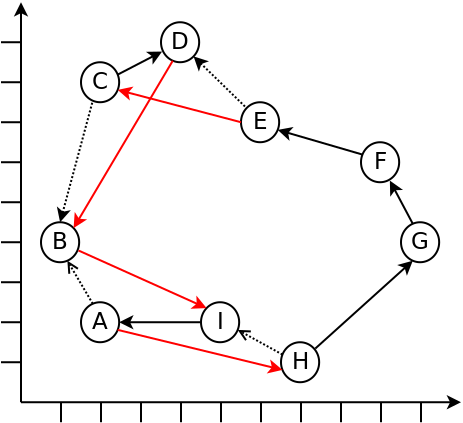
\includegraphics[width=1\linewidth]{figuras/pml/exemplo-rodolfo-2opt-1-7-5-6.png}
        \end{subfigure}
    \end{minipage}
    \begin{minipage}{.475\textwidth}
\begin{Verbatim}[commandchars=\\\{\}]
index:   0  1  2  3  4  5  6  7  8
cidade:  A  \textcolor{red}{H  \textcolor{blue}{F  G}  E  D  C  B}  I
\end{Verbatim}
\begin{gather*}
f(m_1 \circ m_2 \circ s_1)= 3439/18211 \ (PCV/PML) \\
f(m_1 \circ m_2 \circ s_1) = \\
\widehat{m_1}(m_2 \circ s_1) + \widehat{m_2}(s_1) + f(s_1) = \\
509 + 299 + 2631 = 3439 \ (PCV) \\
3872 + 1265 + 13074 = 18211 \ (PML)
\end{gather*}
    \end{minipage}
    \caption{Solução $m_1 \circ m_2 \circ s_1$, com $m_1$ sendo 2-opt(1,7) e $m_2$ sendo 2-opt(5,6).}
    \label{fig:figuraExemplo_m1m2s1}
\end{figure}

Conforme supracitado e ilustrado nas Figuras~\ref{fig:figuraExemplo_m1m2s1} e~\ref{fig:figuraExemplo_m2m1s1} podemos ver que a solução $m_2 \circ m_1 \circ s_1$ não verifica as mesmas propriedades pois apenas $m_1$ não é alterado por $m_2$, desta forma estes movimentos são parcialmente independentes.

\begin{figure}[ht]
    \begin{minipage}{.475\textwidth}
        \begin{subfigure}[t]{1\textwidth} %
            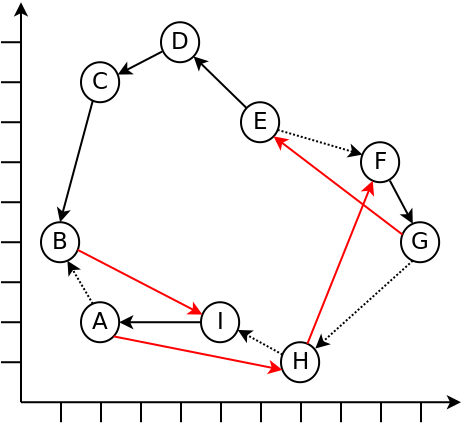
\includegraphics[width=1\linewidth]{figuras/pml/exemplo-rodolfo-2opt-5-6-1-7.png}
        \end{subfigure}
    \end{minipage}
    \begin{minipage}{.475\textwidth}
\begin{Verbatim}[commandchars=\\\{\}]
index:   0  1  2  3  4  5  6  7  8
cidade:  A  \textcolor{red}{H  G  F  E  \textcolor{blue}{C  D}  B}  I
\end{Verbatim}
\begin{gather*}
f(m_2 \circ m_1 \circ s_1) = 3440/17345 \ (PCV/PML) \\
f(m_2 \circ m_1 \circ s_1) = \\
\widehat{m_2}(m_1 \circ s_1) + \widehat{m_1}(s_1) + f(s_1) = \\
300 + 509 + 2631= 3440 \ (PCV) \\
1158 + 3113 + 13074 = 17345) \ (PML)
\end{gather*}
    \end{minipage}
    \caption{Solução $m_2 \circ m_1 \circ s_1$, com $m_2$ sendo 2-opt(5,6) e $m_1$ sendo 2-opt(1,7).}
    \label{fig:figuraExemplo_m2m1s1}
\end{figure}

De fato podemos verificar pela Figura~\ref{fig:figuraExemplo_m2m1s1} que $\widehat{m_2}(s_1)$ = 299/1265 é diferente de $\widehat{m_2}(m_1 \circ s_1)$ = 300/1158.

\subsubsection{Movimentos independentes} \label{subsubsec:movimentosIndependentes}

Movimentos independentes são aqueles que a aplicação de um não altera o valor do outro, o valor do movimento $m_2$ aplicado à solução $m_1 \circ s$ é igual ao valor deste aplicado à solução $s$, a independência de movimentos pode ser definida para movimentos de vizinhanças diferentes.
Em outras palavras movimentos independentes são parcialmente independentes para ambos os lados.
Formalmente temos que dois movimentos $m_1$ e $m_2$ são independentes $m_1 \parallel m_2$ se e somente se:
\begin{equation}
% \begin{align}
m_1 \parallel m_2 \iff \widehat{m_1}(m_2 \circ s) = \widehat{m_1}(s) \;\;\; \land \;\;\; \widehat{m_2}(m_1 \circ s) = \widehat{m_2}(s)
% \end{align}
\end{equation}

\begin{theorem}%[Teorema da independência de movimentos]\label{teo:independenciaMovimentos}
Dois movimentos $m_1$ e $m_s$ são independentes então o valor da solução final não se altera ao alternar a ordem de aplicação dos movimentos, ou seja:
\begin{equation}
m_1 \parallel m_2 \implies f(m_1 \circ m_2 \circ s) = f(m_2 \circ m_1 \circ s)
\end{equation}

\begin{proof}
    Suponhamos que $m_1$ e $m_2$ sejam independentes $\widehat{m_1}(m_2 \circ s) = \widehat{m_2}(s) \land \widehat{m_2}(m_1 \circ s) = \widehat{m_1}(s)$ mas $f(m_1 \circ m_2 \circ s) \neq f(m_1 \circ m_1 \circ s)$.
    \begin{align*}
        f(m_1 \circ m_2 \circ s) \neq & f(m_2 \circ m_1 \circ s) & \textrm{ De }(\ref{eq:movimentoCusto}) \\
        \widehat{m_1}(m_2 \circ s) + f(m_2 \circ s) \neq & \widehat{m_2}(m_1 \circ s) + f(m_1 \circ s) & \textrm{ De }\ (\ref{eq:movimentoCusto}) \\
        \widehat{m_1}(m_2 \circ s) + \widehat{m_2} + f(s) \neq & \widehat{m_2}(m_1 \circ s) + \widehat{m_1} + f(s) & \textrm{ Como } m_1 \parallel m_2 \\
        \widehat{m_1}(s) + \widehat{m_2} + f(s) \neq & \widehat{m_2}(s) + \widehat{m_1} + f(s) & \textrm{ Logo uma contradição } \bot
    \end{align*}
    
    Assim, por \textit{reductio ad absurdum}, temos que se $m_1$ e $m_2$ são independentes então $f(m_1 \circ m_2 \circ s) = f(m_2 \circ m_1 \circ s)$.
\end{proof}
\end{theorem}

Outra propriedade interessante pode ser vista no teorema apresentado a seguir:
\begin{theorem}[Teorema da independência dos movimentos dois a dois]\label{teo:independenciaMovimentos2a2}
Se $m_1 \parallel m_2$ então o valor da solução gerada pela aplicação destes movimentos será igual ao valor anterior da solução somado ao valor dos movimentos.
\begin{equation}
\label{eq:movimentoCustoSomaDois}
m_1 \parallel m_2 \implies f(m_1 \circ m_2 \circ s) = \widehat{m_1}(s) + \widehat{m_2}(s) + f(s)
\end{equation}
\begin{proof}
    Suponhamos que $m_1$ e $m_2$ sejam independentes mas $f(m_1 \circ m_2 \circ s) \neq \widehat{m_1}(s) + \widehat{m_2}(s) + f(s)$.
    \begin{align*}
        f(m_1 \circ m_2 \circ s) \neq & \widehat{m_1}(s) + \widehat{m_2}(s) + f(s) & \textrm{ De } (\ref{eq:movimentoCusto}) \\
        \widehat{m_1}(m_2 \circ s) + f(m_2 \circ s) \neq & \widehat{m_1}(s) + \widehat{m_2}(s) + f(s) & \textrm{ De } (\ref{eq:movimentoCusto}) \\
        \widehat{m_1}(m_2 \circ s) + \widehat{m_2}(s) + f(s) \neq & \widehat{m_1}(s) + \widehat{m_2}(s) + f(s) & \textrm{ Como } m_1 \parallel m_2 \\
        \widehat{m_1}(s) + \widehat{m_2}(s) + f(s) \neq & \widehat{m_1}(s) + \widehat{m_2}(s) + f(s) & \textrm{ Logo uma contradição } \bot
    \end{align*}
    
    Assim, por \textit{reductio ad absurdum}, temos que se $m_1$ e $m_2$ são independentes então $f(m_1 \circ m_2 \circ s) = \widehat{m_1}(s) + \widehat{m_2}(s) + f(s)$.
\end{proof}
\end{theorem}

\subsubsection{Movimentos fortemente independentes -- \emph{strongly independent moves}} \label{subsubsec:movimentosEstritamenteIndependentes}

Dois movimentos $m_1$ e $m_2$ são fortemente independentes quando são independentes e podem ser aplicados simultaneamente a uma solução sem que a alteração feita por um gere conflito na causada pelo outro, a independência de movimentos pode ser definida para movimentos de vizinhanças diferentes.
Formalmente temos que dois movimentos $m_1$ e $m_2$ são fortemente independentes $m_1 \parallel_e m_2$ se e somente se:
\begin{equation}  \label{eq:movimentosIndependentes}
m_1 \parallel_e m_2 \iff m_1(m_2(s)) = m_2(m_1(s)) = m_1 \circ m_2 \circ s = m_2 \circ m_1 \circ s
\end{equation}

% A mesma ideia pode ser aplicada para um conjunto de movimentos $M = \{ m_1, m_2, m_3, ...\}$, são ditos fortemente independentes se para uma solução $s$ qualquer e para todo subconjunto não-vazio $M' = \{ m_1, m_2, m_3, \dots, m_k \} \subseteq M$ temos $m_1 \circ m_2 \circ m_3 \circ ...\circ m_k \circ s = m_2 \circ m_1 \circ m_3 \circ ...\circ m_k \circ s$ para qualquer permutação dos movimentos em $M'$.
% $\widehat{m_1}(s) + \widehat{m_2}(s) + \widehat{m_3}(s) + \dots + \widehat{m_k}(s) = \widehat{m_1}(m_2 \circ m_3 \circ ...\circ m_k \circ s)$. 

Pela Equação~\ref{eq:movimentosIndependentes} pode-se perceber que movimentos fortemente independentes são operações comutativas, pela própria definição.

Assim podemos estender a definição da vizinhança $k$ para:
\begin{equation}  \label{eq:vizinhanca}
N^k(s) = \{ m^k_i \circ s \mid \forall m^k_i \in M^k \}
\end{equation}

Cabe aqui destacar que a independência de movimentos é uma relação dada dois a dois entre os movimentos, logo não existe transitividade na relação de independência destes, ou seja, se temos dois movimentos independentes $m_1 \parallel m_2$ e outro movimento $m_3$ tal que $m_2 \parallel m_3$ então \textbf{não} implica que $m_1 \parallel m_3$.
Pode existir um conflito, logo os movimentos $m_1 \nparallel m_3$ ou seja, seriam conflitantes.
Assim em termos de conflitos entre movimentos podemos escrever:
\begin{equation}
m_1 \parallel m_2 \land m_2 \parallel m_3 \centernot\implies m_1 \parallel m_3
\end{equation}

\begin{proof}
Consideremos o seguinte contraexemplo a seguir para a vizinhança de Swap, sendo os movimentos $Swap(2,3), Swap(3,6), Swap(4,5)$, neste caso podemos ver que $Swap(2,3) \parallel Swap(4,5)$ e que $Swap(4,5) \parallel Swap(3,6)$ contudo $Swap(2,3) \nparallel Swap(3,6)$.
\end{proof}

% Para fins dessa dissertação, por questão de simplificação de notação, deste ponto em diante as referências a \textit{movimentos independentes} estão referenciando \textit{movimentos estritamente independentes}.

\begin{figure}[ht]
    \begin{minipage}{.475\textwidth}
        \begin{subfigure}[t]{1\textwidth} %
            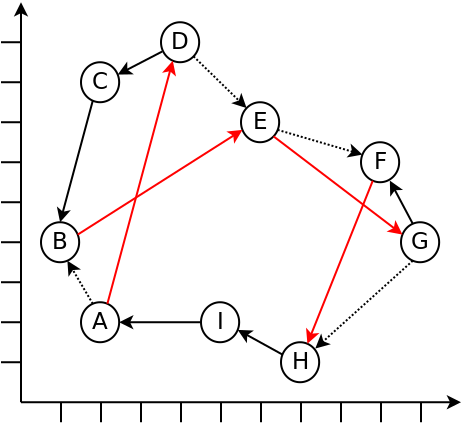
\includegraphics[width=1\linewidth]{figuras/pml/exemplo-rodolfo-2opt-1-3-5-6.png}
        \end{subfigure}
    \end{minipage}
    \begin{minipage}{.475\textwidth}
\begin{Verbatim}[commandchars=\\\{\}]
index:   0  1  2  3  4  5  6  7  8
cidade:  A  \textcolor{green}{D  C  B}  E  \textcolor{blue}{G  F}  H  I
\end{Verbatim}
\begin{gather*}
f(m_2 \circ m_3 \circ s_1): 3734/20487 \ (PCV/PML) \\
f(m_3 \circ m_2 \circ s_1): 3734/20487 \ (PCV/PML) \\
f(m_2 \circ m_3 \circ s_1) = f(m_3 \circ m_2 \circ s_1) \\ \\
\widehat{m_2}(s_1)+\widehat{m_3}(s_1)+f(s_1) = \\
299 + 804 + 2631 = 3734 \ (PCV) \\
1265+6148+13074=20487 \ (PML)
\end{gather*}
    \end{minipage}
    \caption{Solução $m_2 \circ m_3 \circ s_1 = m_3 \circ m_2 \circ s_1$, com $m_2$ sendo 2-opt(5,6) e $m_3$ sendo 2-opt(1,3).}
    \label{fig:figuraExemplo_m2m3s1}
\end{figure}

Note, pela Figura~\ref{fig:figuraExemplo_m2m3s1}, que $m_2 \circ m_3$ opera como um movimento 4-opt (quatro arcos são removidos e inseridos), assim a operação de composição do multi-improvement é capaz de lidar com movimentos de dimensões maiores, em uma única iteração.

\subsubsection{Movimentos conflitantes} \label{subsubsec:movimentosConflitantes}

Há movimentos com conflito de escrita na representação (estrutura de dados) da solução, portanto não é possível aplicá-los simultaneamente. Nesse caso, diz-se que eles são dependentes de ordem (order-dependent moves) ou, simplesmente, conflitantes.

Por exemplo, como $m_1$=2opt(1,7) e $m_3$=2opt(1,3) são conflitantes, $m_1 \circ m_3 \circ s_1$ e $m_3 \circ m_1 \circ s_1$ são soluções estruturalmente distintas, conforme pode ser visto na Figura~\ref{fig:figuraExemplo_m1m3s1}.

\begin{figure}[ht]
    \begin{minipage}{.475\textwidth}
        \begin{subfigure}[t]{1\textwidth} %
            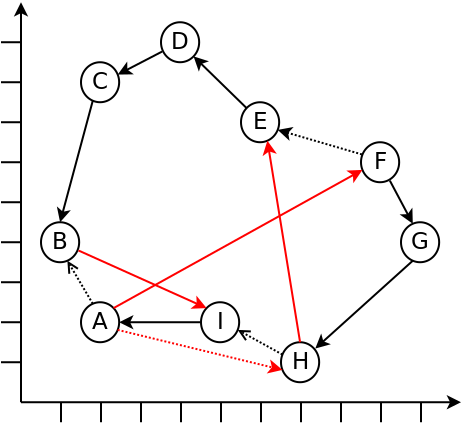
\includegraphics[width=1\linewidth]{figuras/pml/exemplo-rodolfo-2opt-1-7-1-3.png}
        \end{subfigure}
    \end{minipage}
    \begin{minipage}{.475\textwidth}
\begin{Verbatim}[commandchars=\\\{\}]
index:   0  1  2  3  4  5  6  7  8
cidade:  A  \textcolor{red}{H  G  F  E  \textcolor{green}{B  C  D}}  I
\end{Verbatim}
\begin{gather*}
f(m_1 \circ m_3 \circ s_1) : 3700/18395 \ (PCV/PML)\\
\widehat{m_1}(m_3 \circ s_1) + \widehat{m_3}(s_1) + f(s_1) =\\
265+804+2631=3700 \ (PCV) \\
827+6148+13074=18395 \ (PML)
\end{gather*}
    \end{minipage}
    \caption{Solução $m_1 \circ m_3 \circ s_1$, com $m_1$ sendo 2-opt(1,7) e $m_3$ sendo 2-opt(1,3).}
    \label{fig:figuraExemplo_m1m3s1}
\end{figure}

\begin{figure}[ht]
    \begin{minipage}{.475\textwidth}
        \begin{subfigure}[t]{1\textwidth} %
            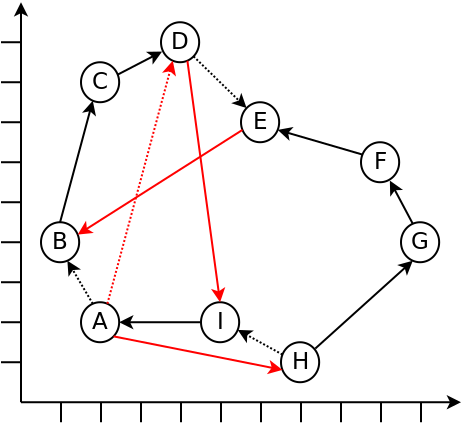
\includegraphics[width=1\linewidth]{figuras/pml/exemplo-rodolfo-2opt-1-3-1-7.png}
        \end{subfigure}
    \end{minipage}
    \begin{minipage}{.475\textwidth}
\begin{Verbatim}[commandchars=\\\{\}]
index:   0  1  2  3  4  5  6  7  8
cidade:  A  \textcolor{green}{F  G  H}  \textcolor{red}{E  D  C  B}  I
\end{Verbatim}
\begin{gather*}
f(m_3 \circ m_1 \circ s_1) = 3728/20403 \ (PCV/PML) \\
\widehat{m_3}(m_1 \circ s_1)+\widehat{m_1}(s_1)+f(s_1) = \\
588+509+2631=3728 \ (PCV) \\
4216+3113+13074=20403 \ (PML)
\end{gather*}
    \end{minipage}
    \caption{Solução $m_3 \circ m_1 \circ s_1$, com $m_3$ sendo 2-opt(1,3) e $m_1$ sendo 2-opt(1,7).}
    \label{fig:figuraExemplo_m3m1s1}
\end{figure}

Naturalmente, como $m_1$ e $m_3$ são conflitantes (vide Figura~\ref{fig:figuraExemplo_m3m1s1}), $\widehat{m_3}(m_1 \circ s_1) \neq \widehat{m_3}(s_1)$ e $\widehat{m_1}(m_3 \circ s_1) \neq \widehat{m_1}(s_1)$.
Também é interessante de notar que a composição executa um movimento 3-opt, então mesmo que não seja permitido na composição do 2-opt pode ser alcançado ao utilizar alguma outra vizinhança num processo simultâneo (generalized multi-improvement).

% Estou achadno a prova do teorema muito fraca
% % Igor coloquei isso aqui como um Teorema, não sei se é muito ambicioso da minha parte
% 
\begin{theorem}[Teorema da independência de movimentos]\label{teo:independenciaMovimentos}
Seja um conjunto $M'$ com movimentos livres de contexto em que todos os movimentos são independentes entre si dois a dois, ou seja $m_i \parallel m_j \mid \forall m_i, m_j \in M'$, com $m_i \ne m_j$.
E seja $s'$ a solução dada pela aplicação de todos os movimentos à solução inicial $s$, logo o valor da solução resultante $s'$ será dado pelo somatório do valor de cada movimento. Assim, pode-se escrever:

% \begin{align*} \label{eq:teo:independenciaMovimentos}
% m_1 \parallel m_2 \implies& s' = m_1 \circ m_2 \circ s \\
% m_1 \parallel m_2 \implies& f(s') = \widehat{m_1}(s) + \widehat{m_2}(s) + f(s) \\
% \end{align*}

% \begin{align*}
\begin{equation}
    \label{eq:teo:independenciaMovimentos}
    \begin{split}
        m_i \parallel m_j, \forall m_i, m_j \in M' \implies& s' = m_1 \circ m_2 \circ \dots \circ m_n \circ s \\
        m_i \parallel m_j, \forall m_i, m_j \in M' \implies& f(s') = f(s) + \widehat{m_1}(s) + \widehat{m_2}(s)+ \widehat{m_3}(s) + \dots + \widehat{m_n}(s) \\
        m_i \parallel m_j, \forall m_i, m_j \in M' \implies& f(s') = f(s) + \sum_i^n{\widehat{m_i}(s)}
    \end{split}
\end{equation}
% \end{align*}
\end{theorem}

\begin{proof}\label{proof:independenciaMovimentos}
% ---
% Prova por contradição
% ---
Suponhamos um conjunto $M = \{ m_1, m_2, \dots, m_n \}$ com $n$ movimentos independentes dois a dois mas $f(m_1 \circ m_2 \circ \dots \circ m_n \circ s) \neq f(s) + \widehat{m_1}(s) + \widehat{m_2}(s)+ \widehat{m_3}(s) + \dots + \widehat{m_n}(s)$.

\begin{align*}
    f(m_1 \circ m_2 \circ \dots \circ m_n \circ s) \neq f(s) + \widehat{m_1}(s) + \widehat{m_2}(s) + \dots + \widehat{m_n}(s) & \\
    \widehat{m_1}(m_2 \circ \dots \circ m_n \circ s) + f(m_2 \circ \dots \circ m_n \circ s) \neq f(s) + \widehat{m_1}(s) + \widehat{m_2}(s) + \dots + \widehat{m_n}(s) & \ [1] \\
    \widehat{m_1}(s) + f(m_2 \circ \dots \circ m_n \circ s) \neq f(s) + \widehat{m_1}(s) + \widehat{m_2}(s) + \dots + \widehat{m_n}(s) & \\
    \widehat{m_1}(s) + \widehat{m_2}(m_3 \circ \dots \circ m_n \circ s) + f(m_3 \circ \dots \circ m_n \circ s) \neq f(s) + \widehat{m_1}(s) + \widehat{m_2}(s) + \dots + \widehat{m_n}(s) & \ [2] \\
    \widehat{m_1}(s) + \widehat{m_2}(s) + f(m_3 \circ \dots \circ m_n \circ s) \neq f(s) + \widehat{m_1}(s) + \widehat{m_2}(s) + \dots + \widehat{m_n}(s) & \\
    \vdots & \\
    \widehat{m_1}(s) + \widehat{m_2}(s) + \dots + \widehat{m_n}(s) + f(s) \neq f(s) + \widehat{m_1}(s) + \widehat{m_2}(s) + \dots + \widehat{m_n}(s) & \ [3] \\
\end{align*}

Os passos acima se dão conforme:
\begin{align*}
[1] \ & m_1 \parallel m_i \mid \forall m_i \in M \\
[2] \ & m_2 \parallel m_i \mid \forall m_i \in M \\
[3] \ & \textrm{Logo temos uma contradição} \bot
\end{align*}

Desta forma, por \textit{reductio ad absurdum} demonstramos que se os movimentos são independentes então o valor da solução resultante se dará pelo somatório da solução anterior com o valor dos movimentos.

% ---
% Indução
% ---
% Pela Equação~\ref{eq:movimentoCustoSomaDois} temos que $f(m_1 \circ m_2 \circ s) = \widehat{m_1}(s) + \widehat{m_2}(s) + f(s)$, supondo por hipótese de indução que $f(m_1 \circ m_2 \circ \dots \circ m_n \circ s) = f(s) + \widehat{m_1}(s) + \widehat{m_2}(s) + \dots + \widehat{m_n}(s)$

% \begin{align*}
%     f(m_1 \circ m_2 \circ \dots \circ m_n \circ m_{n+1} \circ s) = & f(m_{n+1} \circ m_1 \circ m_2 \circ \dots \circ m_n \circ s) \\
%     f(m_1 \circ m_2 \circ \dots \circ m_n \circ m_{n+1} \circ s) = & \widehat{m_{n+1}}(m_1 \circ m_2 \circ \dots \circ m_n \circ s) + f(m_1 \circ m_2 \circ \dots \circ m_n \circ s) \\
% \end{align*}

% % \widehat{m_1}(s) + \widehat{m_2}(s) + \dots + \widehat{m_n}(s) + f(s)
% Fazendo $s_2 = m_2 \circ \dots \circ m_n \circ s$.
% \begin{align*}
%     f(m_1 \circ m_2 \circ \dots \circ m_n \circ m_{n+1} \circ s) = & \widehat{m_{n+1}}(m_1 s_2) + f(m_1 \circ m_2 \circ \dots \circ m_n \circ s) \\
%     f(m_1 \circ m_2 \circ \dots \circ m_n \circ m_{n+1} \circ s) = & \widehat{m_{n+1}}(s_2) + f(m_1 \circ m_2 \circ \dots \circ m_n \circ s)
% \end{align*}

% Pois $m_{n+1} \parallel m_1$, fazendo agora $s_3 = m_3 \circ \dots \circ m_n \circ s$.
% \begin{align*}
%     f(m_1 \circ m_2 \circ \dots \circ m_n \circ m_{n+1} \circ s) = & \widehat{m_{n+1}}(m_2 \circ \dots \circ m_n \circ s) + f(m_1 \circ m_2 \circ \dots \circ m_n \circ s)\\
%     f(m_1 \circ m_2 \circ \dots \circ m_n \circ m_{n+1} \circ s) = & \widehat{m_{n+1}}(m_2 \circ s_3) + f(m_1 \circ m_2 \circ \dots \circ m_n \circ s)\\
%     f(m_1 \circ m_2 \circ \dots \circ m_n \circ m_{n+1} \circ s) = & \widehat{m_{n+1}}(s_3) + f(m_1 \circ m_2 \circ \dots \circ m_n \circ s)\\
%     \vdots \\
%     f(m_1 \circ m_2 \circ \dots \circ m_n \circ m_{n+1} \circ s) = & \widehat{m_{n+1}}(s) + f(m_1 \circ m_2 \circ \dots \circ m_n \circ s)\\
%     f(m_1 \circ m_2 \circ \dots \circ m_n \circ m_{n+1} \circ s) = & \widehat{m_{n+1}}(s) + \widehat{m_1}(s) + \widehat{m_2}(s) + \dots + \widehat{m_n}(s) + f(s)
% \end{align*}

% Logo, por indução finita temos que $m_i \parallel m_j, \forall m_i, m_j \in M' \implies f(s') = f(s) + \sum_i^n{\widehat{m_i}(s)}$.

\end{proof}


\subsection{First Improvement vs Best Improvement} \label{subsec:firstBestImprovement}

As estratégias \textit{First Improvement} (Primeira melhora) e \textit{Best Improvement} (Melhor melhora) recebem como parâmetro a solução da iteração corrente para gerar seus vizinhos e escolhem uma solução a ser retornada conforme um critério específico, a saber, a primeira solução a melhorar a atual e a melhor solução encontrada na vizinhança, respectivamente.

\begin{algorithm}[htpb]
\caption{First Improvement para um problema de minimização}
\label{alg:firstImprovement}
\begin{algorithmic}[1]
    \Function{FirstImprovement}{Solução: $s$, Operador de vizinhança: $x$}
        % \For{$s' \in N^x(s)$} \Comment{Para cada solução $s'$ vizinha de $s$}
        %     \If{$f(s') < f(s)$} \Comment{Se a solução for melhor que a atual}
        %         \Return{$s'$}
        %     \EndIf
        % \EndFor
        \For{$m_i \in M$} \Comment{Para cada movimento $m_i \in M$}
            \If{$\widehat{m_i}(s) < 0$} \Comment{Se a solução for melhor que a atual}
                \Return{$m_i \circ s$}
            \EndIf
        \EndFor
        \Return{$s$} \Comment{Caso não consiga melhorar retorna a própria solução}
    \EndFunction
\end{algorithmic}
\end{algorithm}

Podemos ver o pseudocódigo do \textit{First Improvement} no Algoritmo~\ref{alg:firstImprovement} que consiste de enumerar os vizinhos até encontrar o primeiro que seja melhor que a solução atual, este então é retornado como resposta do método.
O método de \textit{Best Improvement} (Algoritmo~\ref{alg:bestImprovement}) consiste em enumerar toda a vizinhança guardando a informação do melhor encontrado até o momento, e então retornar o melhor resultado encontrado.

\begin{algorithm}[htpb]
\caption{Best Improvement para um problema de minimização}
\label{alg:bestImprovement}
\begin{algorithmic}[1]
    \Function{BestImprovement}{Solução: $s$, Operador de vizinhança: $x$}
        % \Let{$s^{best}$}{$s$} \Comment{Melhor solução encontrada}
        % \For{$s' \in N^x(s)$} \Comment{Para cada solução $s'$ vizinha de $s$}
        %     \If{$f(s') < f(s)$} \Comment{Se a solução for melhor que a atual altera a melhor solução encontrada}
        %         \Let{$s^{best}$}{$s'$}
        %     \EndIf
        % \EndFor
        \Let{$s^{best}$}{$s$} \Comment{Melhor solução encontrada}
        \For{$m_i \in M$} \Comment{Para cada movimento $m_i \in M$}
            \If{$\widehat{m_i}(s) < f(s^{best}) - f(s)$} \Comment{Se a solução for melhor que a atual altera a melhor solução encontrada}
                \Let{$s^{best}$}{$m_i \circ s$}
            \EndIf
        \EndFor
        \Return{$s^{best}$} \Comment{Retorna a melhor solução encontrada}
    \EndFunction
\end{algorithmic}
\end{algorithm}

O \textit{First Improvement} pode ser uma opção ao método de \textit{Best Improvement} quando a enumeração de toda a vizinhança é uma atividade muito custosa.
% Posso afirmar isso?
Embora não haja um paralelo para a definição matemática formal da solução $s'$ retornada pelo \textit{First Improvement} esta pode ser definida para o \textit{Best Improvement} de maneira simples por $s' \in N^x(s) \mid f(s') < f(s), \forall s \in N^x(s)$, o que, como veremos a seguir na seção~\ref{sec:otimoLocalGlobal}, corresponde ao ótimo local para a solução $s$ segundo a vizinhança $x$.
Em termos de movimento temos $s' = m' \circ$ com $\widehat{m'}(s) < \widehat{m_i}(s) \mid \forall m_i \in M$.

\subsection{Random Selection}

Nesta estratégia \textit{Random Selection} (Escolha Aleatória) é selecionada uma solução aleatoriamente entre aquelas que melhoram a solução atual.

\begin{algorithm}[htpb]
\caption{Random Selection para um problema de minimização}
\label{alg:randomSelection}
\begin{algorithmic}[1]
    \Function{RandomSelection}{Solução: $s$, Operador de vizinhança: $x$}
        \Let{$S_{imp}$}{$\emptyset$} \Comment{Conjunto com soluções de melhora}
        \For{$m_i \in M$} \Comment{Para cada movimento $m_i \in M$}
            \If{$\widehat{m_i}(s) < 0$} \Comment{Se a solução for melhor que a atual}
                \Let{$S_{imp}$}{$S_{imp} \cup \{ m_i \circ s\}$} \label{alg:randomSelection:salvaMelhora} \Comment{Adiciona ao conjunto de soluções de melhora}
            \EndIf
        \EndFor
        \Return{$Any(S_{imp})$} \Comment{Retorna uma das soluções de melhora}
    \EndFunction
\end{algorithmic}
\end{algorithm}

A estratégia \textit{Random Selection} (mostrada no Algoritmo~\ref{alg:randomSelection}) navega pelas soluções e na mantém as melhores soluções que melhoram a solução atual, conforme linha~\ref{alg:randomSelection:salvaMelhora}, para ao final retornam uma deste grupo.

\subsection{Multi Improvement}

Uma alternativa ao \emph{Best Improvement}, \emph{First Improvement} e ao \emph{Random Selection} é o \emph{Multi Improvement}~\cite{rios2015}.
A ideia é combinar um conjunto de movimentos independentes e executá-los simultaneamente sobre a solução de entrada.
Note que, embora consista na aplicação de diversos movimentos, somente uma única solução vizinha é gerada.
O \emph{Multi Improvement} pode ser utilizado em qualquer contexto que o \emph{Best Improvement} ou \emph{First Improvement} se encaixe (etapa de Exploração de Vizinhança ou {\it Neighborhood Exploration}), porém caso só exista um único movimento independente na vizinhança, ele terá comportamento equivalente ao Best Improvement.
Assim a solução $s'$ retornada por uma iteração do \emph{Multi Improvement} após ser aplicado a uma solução $s$ é dada por $s' = m_1 \circ m_2 \circ \dots m_k \circ s$ com os movimentos independentes $\{ m_1, m_2, \dots, m_k \} \subset M$.

O \emph{Multi Improvement} se encaixa particularmente bem com o conceito de \emph{SIMD} (\emph{Single Instruction Multiple Data}), presente nas GPUs, sendo sua complexidade similar ao \emph{Best Improvement} (todos movimentos da vizinhança são enumerados), seguido de uma etapa de junção (ou {\it merge}) dos movimentos independentes.
Podem existir cenários em que o \emph{Best Improvement} seja mais eficiente (com poucos movimentos independentes), embora já tenha sido demonstrado na literatura que mesmo casos com apenas dois movimentos independentes acabam mais promissores no \emph{Multi Improvement} do que no \emph{Best Improvement}. % Não seria importante colocar a referência disso?

\subsection{Passo iterativo} \label{subsec:passoIterativo}
% Posso fazer essa definição que estou fazendo aqui?
% Pensei em fazer isso para facilitar explicar algumas coisas mais pra frente

Em geral, um algoritmo de busca local é um processo iterativo pesado que tem como objetivo encontrar uma solução melhor que a atual dentro de um espaço de busca.
A solução recebida como entrada pode ser aleatória ou advinda de alguma heurística construtiva, a intenção do processo é aprimorar o resultado encontrado.

Cada iteração da busca local tenta encontrar a melhor solução mediante alguma alteração na solução atual, então o processo se repete na solução gerada até que nenhuma melhora seja possível.

\begin{algorithm}[htpb]
\caption{Busca local definida de forma genérica}
\label{alg:localSearch}
\begin{algorithmic}[1]
    \Function{LocalSearch}{Solução: $s$}
        \While{$f(Alterar(s)) < f(s)$} \Comment{Cada iteração corresponde a um passo iterativo da busca local}
            \Let{s}{$Alterar(s)$}
        \EndWhile
        \Return{$s$} \Comment{Retorna a melhor solução encontrada}
    \EndFunction
\end{algorithmic}
\end{algorithm}

Supondo que $Alterar(s)$ (apresentado do Algoritmo~\ref{alg:localSearch}) retorna uma solução melhor que a atual segundo alguma alteração, convencionemos então chamar de \textbf{passo iterativo} cada iteração da busca local em que o processo obtém uma solução melhor que a atual e salva o melhor resultado encontrado até o momento.
Assim para uma solução $s$ o passo iterativo é dado pela Equação~\ref{eq:passoIterativo}.

\begin{equation} \label{eq:passoIterativo}
\rho(s) = min(s, Alterar(s)) \implies f(\rho(s)) \le f(s)
\end{equation}

\section{Ótimo global vs Ótimo local} \label{sec:otimoLocalGlobal}

O ótimo global e ótimo local são exemplificados na Figura~\ref{fig:espacoDeBusca}.
Uma solução $s^* \in S$ é dita \textbf{ótimo global} para um problema $\Pi$ quando não existe outra solução viável $s'$ com melhor valor de função objetivo, formalmente temos que $s^*$ é ótimo global quando:
\begin{itemize}
    \item $\forall s' \in S \mid f(s') \le f(s^*), s' \neq s^* $ para um problema de maximização;
    \item $\forall s' \in S \mid f(s') \ge f(s^*), s' \neq s^* $ para um problema de minimização.
\end{itemize}

Considere uma busca local de \textit{Best Improvement} $H$ para o problema $\Pi$ sobre a estrutura de vizinhança $N^x$, após aplicar $H$ a uma solução inicial $s^0 \in S$ é obtido um conjunto de soluções $N^x(s^0)$ vizinhas, assim o \textbf{ótimo local} (\textit{mínimo local}) segundo a vizinhança $N^x$ para a solução $s^0$ é dado por:
\begin{itemize}
    \item $s'' \in N^x(s^0) \mid f(s'') < f(s'), \forall s' \in N^x(s^0), s'' \neq s'$, para um problema de minimização;
    \item $s'' \in N^x(s^0) \mid f(s'') > f(s'), \forall s' \in N^x(s^0), s'' \neq s'$, para um problema de maximização.
\end{itemize}

Em linhas gerais um \textbf{ótimo local} é a solução com melhor valor de função objetivo para um contexto local, seja uma vizinhança ou o conjunto imagem de uma heurística.

\section{Meta-heurísticas} \label{sec:metaHeuristicas}

Uma meta-heurísticas diferencia-se de uma heurística por não ser acoplada a um problema específico ou classe de problemas.
Meta-heurísticas fazem uso de artifícios capazes de encontrar soluções e aprimorar as já encontradas enquanto procuram escapar de mínimos locais.
Na literatura são utilizadas em trabalhos que tratam de problemas da classe NP-Difícil devido a simplicidade de implementação e a intratabilidade da solução exata de tais problemas.
Assim, esses algoritmos são ferramentas robustas para serem aplicadas na resolução prática de problemas de otimização combinatória, sendo uma alternativa quando o respectivo algoritmo exato não é conhecido ou exige um alto tempo de execução \cite{glover2006handbook}.

As meta-heurísticas evoluem iterativamente conforme a parametrização fornecida até atingir um \textbf{Critério de Parada}, que pode também estar sujeito aos parâmetros do método.
O critério de parada, em geral, está associado ao número de iterações, tempo de execução, um parâmetro de qualidade ou número de iterações sem melhora.

\section{Dataflow} \label{sec:conceitosDataflow}
% Essa parte tá bem próxima da tese do Marzulo

Atualmente os processadores no mercado de computadores seguem, em geral, o modelo de \textit{Von Neumann}.
No referido modelo, a execução das instruções é guiada por um fluxo de controle, ou seja, segundo a ordem que aparecem no programa, desta forma se faz necessário um \textit{Program Counter} (Contador de Programa) para indicar qual a próxima instrução a ser executada.
O contador também pode ser alterado por instruções de desvio, e laços de repetição ou qualquer tipo de comando de execução condicional.

Note que este modelo é intrinsecamente sequencial. No entanto, tenta-se resgatar paralelismo em nível de instruções com técnicas como pipelining~\cite{patterson2003computerOrganization}, predição de desvio~\cite{patterson2003computerOrganization} e renomeamento de registradores~\cite{patterson2012}.

O modelo dataflow~\cite{2468, Swanson2003, 642111, Davis:1978:ASM:800094.803050, 714523, Shimada:1986:EPD:17356.17383, Kishi:1983:DDD:1067651.801661, Grafe:1989:EDP:74925.74930, 134511, Swanson:2007:WA:1233307.1233308} expõe paralelismo de forma natural.
Neste modelo, as instruções são executadas de acordo com o fluxo de dados, ou seja, assim que todos os seus operandos de entrada estiverem disponíveis.

No modelo dataflow os programas são escritos como um grafo de fluxo de dados onde os nós representam as instruções e as arestas direcionadas indicam as dependências de dados.
Assim $A \rightarrow B$ indica que $A$ produz um dado que é enviado como entrada para $B$ após ter sido processado.
Cabe lembrar que este modelo é adotado nas máquinas de Von Neumann para extrair paralelismo ao implementar o mecanismo de execução fora-de-ordem com escalonamento dinâmico baseado em fluxo de dados~\cite{tomasulo}, contudo limitado o paralelismo pela emissão das instruções que permanece seguindo o fluxo de controle.
Numa arquitetura que segue totalmente o fluxo de dados as instruções não são emitidas segundo se apresentam no programa, instruções distintas podem executar concorrentemente.

Na Figura~\ref{fig:dataflowExemploPython} pode ser visto um programa simples, à esquerda é mostrado o código e à direita sua tradução no grafo de fluxo de dados associado, note que as instruções de soma e multiplicação podem ser executadas em paralelo ou qualquer ordem sem alterar o resultado final.

\begin{figure}
    \centering
    \begin{minipage}{.3\textwidth}
        \centering
\begin{minted}{python}
a = 10
b = 9
c = 3
d = 8
e = a * b
f = c + d
if e > f:
  g = (a - b) * a
else:
  g = (c - d) * d
\end{minted}
    \end{minipage}
    \begin{minipage}{.675\textwidth}
        \centering %width=.655\linewidth
        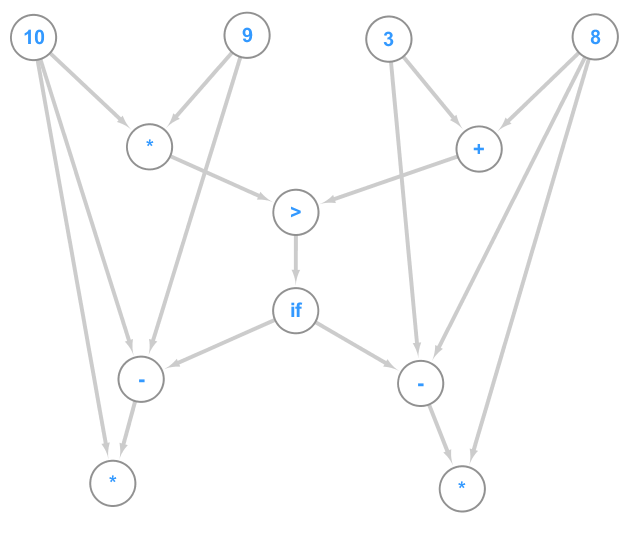
\includegraphics[scale=.7]{figuras/dataflow/pythonCodeDf.png}
    \end{minipage}
    \caption{Exemplo de conversão código para grafo de dependências.
    À esquerda pode ser visto um trecho de código em \emph{python} ao passo que à direita é exibido o grafo dataflow associado.}
    \label{fig:dataflowExemploPython}
\end{figure}

\subsection{Sucuri} \label{sect:sucuri}

Sucuri~\cite{sucuri-original} é uma biblioteca minimalística Dataflow para a linguagem Python que permite aos programadores explorarem o paralelismo mais naturalmente pela execução dataflow em máquinas que seguem a arquitetura Von Neumann.
Sucuri permite uma execução transparente em um \emph{cluster} de máquinas ao fazer uso do mecanismo de serialização de objetos em Python (\emph{Pickle}).

Conceitualmente, um grafo dataflow é composto de nós que representa tarefas, que podem ser de grão fino (como instruções) ou grão grosso (como funções ou procedimentos).
As arestas que conectam os nós representam dependências de dados, significando que um nó de origem irá produzir um resultado que será utilizado por um nó de destino.
Quando um certo nó recebe todas as entradas necessárias (são satisfeitas todas as suas dependências) este pode ser enfileirado para executar o seu processamento.

A Figura~\ref{fig:arch} mostra a estrutura do Sucuri, onde é possível observar três componentes principais:
\texttt{Graph} (Grafo), \texttt{Scheduler} (Escalonador) e o \texttt{Worker} (Operário).

O \texttt{Graph} é apenas o grafo de dependências da aplicação dataflow, podendo ser visto como um contêiner de nós, onde cada um contêm:
\begin{itemize}
    \item{A lista de entradas de dados até o momento.
    Quando todos os operandos são recebidos ocorre um \emph{matching} e a execução do nó será disparada;}
    \item{A função (computação) que deve ser executada quando for o momento para este nó;}
    \item{Uma lista de nós de destino que devem receber o resultado produzido na sua computação;}
    \item{Atributos específicos, como um identificador único que pode ser usado para atribuição de trabalho para um conjunto específico de nós (como numa abordagem \emph{fork-join}).}
\end{itemize}

Quando é usado em um \emph{cluster} de computadores, cada componente supracitado é replicado em cada máquina do \emph{cluster}, com exceção do \texttt{Scheduler}, o que implica que a Sucuri adota um \emph{pool} de tarefas centralizado.
Em~\cite{sucuri-distribuida} os autores da Sucuri implementaram e avaliaram uma versão da biblioteca utilizando um escalonador distribuído, contudo esta versão ainda não foi utilizada nesse trabalho.

\begin{figure}[htbp]
    \centering
    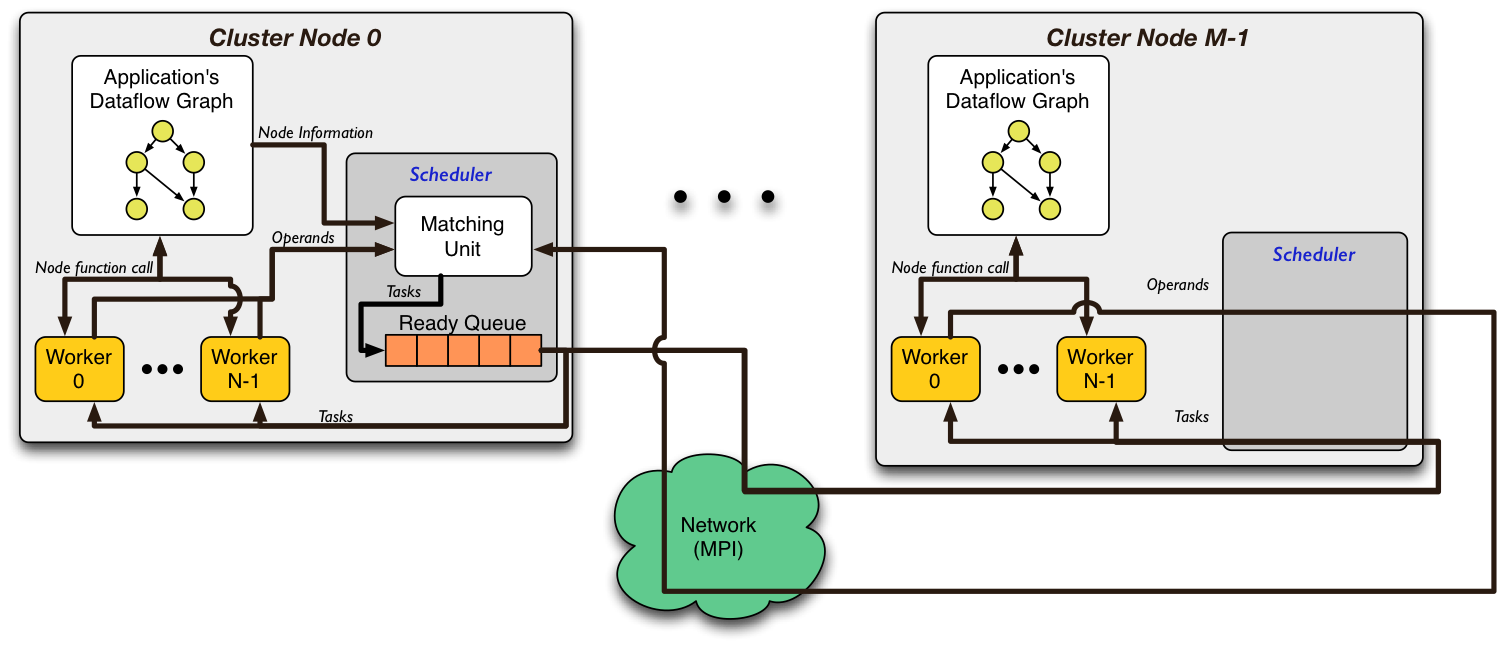
\includegraphics[scale=0.65]{figuras/dataflow/SucuriArchitectureHorizonal.png}
    \caption{A Arquitetura da Sucuri (de~\cite{sucuri-original}).
    A mesma estrutura é replicada em cada nó, entretanto apenas no \texttt{Scheduler} do nó 0 do cluster contem o \texttt{Matching Unit} e o \texttt{Ready Queue}.
    Este é responsável por receber operandos dos \texttt{workers} locais e de outros \texttt{Schedulers}, além disso este gera as tarefas para serem enfileiradas no \texttt{Ready Queue}.}
    \label{fig:arch}
\end{figure}

O \texttt{Scheduler} (escalonador) principal, situado no nó 0 do \emph{cluster}, é composto por uma \texttt{Matching Unit}, uma \texttt{Ready Queue} (fila de prontos) e uma \texttt{Waiting Queue} (fila de espera).
Este é responsável por entregar todos os operandos aos seus respectivos nós de destino no grafo.
Se ocorre um \emph{match}, isto é, todas as dependências de dados são satisfeitas para um nó, então uma tarefa é criada e inserida na \texttt{Ready Queue}.
Quando os \texttt{workers} estiverem ociosos estes vão requisitar uma tarefa para o \texttt{Scheduler} que será buscada da \texttt{Ready Queue}.
O \texttt{Scheduler} situado em outros nós do cluster são mais simples e apenas encaminham tarefas do \texttt{Scheduler} principal para seus \texttt{workers} locais e operandos de seus \texttt{workers} para o \texttt{Scheduler} principal.
O grafo é replicado em todos os nós do \emph{cluster} mas apenas o grafo do nó 0 pode receber operandos do \texttt{Scheduler} principal.

Toda a comunicação intra-nó entre os componentes principais citados acima é realizada via memória compartilhada e entre \texttt{Schedulers} de nós diferentes é feita via interface.

Cada nó do grafo da Sucuri é associado a uma função que pode ser implementada pelos programadores e passada para estes no momento da criação do grafo dataflow.
Após instanciar os nós, o programador pode criar as ligações entre estes usando o método \texttt{add\_edge()} do nó que cria uma dependência no grafo dataflow.
Quando o escalonador dispara a execução de uma tarefa num certo worker, este vai chamar a execução do método \texttt{run()} do respectivo nó para aquela tarefa.
Na maioria dos casos, este método \texttt{run()} vai atuar como um invólucro que chama a execução da função associada ao nó no momento da construção do grafo, passando os operandos como parâmetro e ao final irá enviar os valores retornados pela função para o escalonador.

De mais a mais Sucuri também provê um conjunto especial de nós que podem auxiliar o programador a elaborar aplicações que sigam alguns padrões de paralelismo.
Por exemplo, uma aplicação que envolva \emph{pipeline} para Sucuri é apresentada na Figura~\ref{fig:pipeline}.
O painel $A$ mostra o grafo representando este padrão e o painel $B$ o código Sucuri para essa operação.
Note como novos nós são criados (linhas 11-13), adicionados ao grafo (linhas 17-19) e como as arestas conectando os nós são definidas (linhas 21 e 22).
Perceba também a instanciação no escalonador (linha 6) e como este é inicializado após o grafo dataflow ter sido definido (linha 23).

A Figura~\ref{fig:pipeline} também aponta como o nó especial \texttt{Source} recebe um objeto \emph{iterador} Python (por exemplo uma lista ou um descritor de arquivo) na sua instanciação.
Durante a execução do programa, o método \texttt{run()} do nó \emph{Source} será disparado apenas uma vez visto que este é a raiz, i.e., não possui operandos de entrada no grafo e é usado para iniciar a computação.
Todavia, a execução deste método vai durar até que todo o conteúdo do objeto iterador tenha sido consumido.
Por padrão o nó \texttt{Source} vai executar um laço sobre o objeto iterador e produzirá múltiplas saídas (mensagens) que irão disparar a execução do pipeline múltiplas vezes.

Veja também que o último nó do pipeline é o nó especial \texttt{Serializer}, que é responsável por escrever os dados no arquivo.
É possível que os dados produzidos pelo nó \texttt{Source} sejam processados fora de ordem pelo segundo nó uma vez que múltiplas tarefas podem ser escalonadas em workers diferentes.
Por conseguinte, é necessário reordenar os dados antes de os escrever no arquivo, no nó \texttt{Serializer}.
Para tanto, os dados produzidos pelo nó \texttt{Source} precisam estar encapsulados num objeto \texttt{TaggedValue} que contem uma atributo \texttt{tag}, indicando sua posição na ordem do conjunto de dados.
O nó no intermédio também vai enviar os dados filtrados dentro do objeto \texttt{TaggedValue}, com a mesma tag do pedaço de dados que recebeu.
O nó \texttt{Serializer} então ao receber os dados do nó de filtro, vai armazená-los num \emph{buffer} ordenando de acordo com a tag.
Se a tag do último fragmento de dados recebido corresponde ao próximo a ser escrito no arquivo então o nó \texttt{Serializer} obtém os dados do \emph{buffer} ordenando e escreve no arquivo até que haja uma lacuna na ordenação, i.e. a porção de dados que é a próxima a ser escrita ainda não chegou ao \emph{buffer}.
Se os dados recebidos pelo \texttt{Serializer} estão fora de ordem, o nó apenas os armazena no \emph{buffer} ordenado e aguarda por mais dados.
O método \texttt{pin\(\)} é usado para fixar um nó a um determinado worker, o que fará com que este seja executado apenas por este worker específico.
No caso do exemplo, foram fixados os nós que fazem operações de E\/S no disco aos workers que tem acesso direto ao disco.

\begin{figure}[htbp]
    \centering
    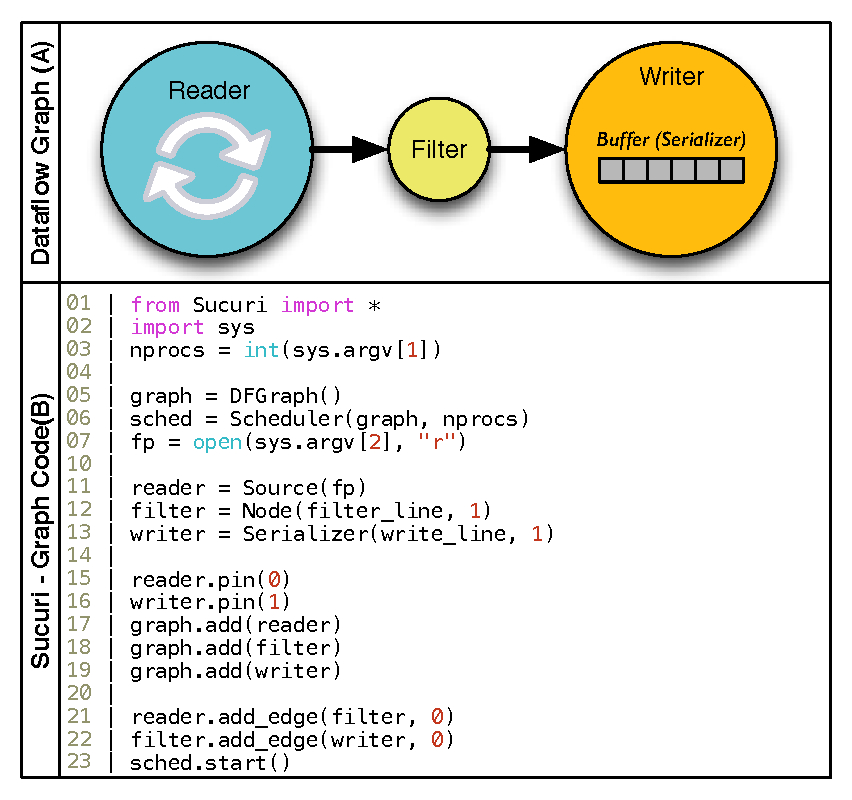
\includegraphics[scale=0.75]{figuras/dataflow/pipeline.eps} 
    \caption{\emph{Pipelining} com Sucuri. 
    %The data is read from the disk by \texttt{Reader} node encapsulated in a \texttt{TaggedValue} object while a filter is applied by \texttt{Filer} node in a data read previously. As the \texttt{Filter} finish, the \texttt{Writer} node receives and store them in buffer sorted according to the tag. If the tag of the last piece of data received corresponds to the next data to be written to the file, the \texttt{Writer} node proceeds to pop data from the sorted buffer and write to the file.
    Painel $A$ mostra um grafo de uma aplicação dataflow, o painel $B$ descreve o grafo usando a Sucuri.}
    \label{fig:pipeline}
\end{figure}

Um recurso de modelagem interessante que foi usado nesse trabalho consiste em explorar a programação em grão grosso usando a Sucuri junto com a computação em grão fino em GPU, resultando assim numa computação heterogênea Dataflow/Von Neumann, com nós dataflow executando operações de alta performance em GPU.
Esta estratégia permite uma grande flexibilidade para o design de insólitos algoritmos, com maior simplicidade do que adotando um único paradigma de computação (dataflow ou Von Neumann).

\section{RVND} \label{sec:rvndClassico}

O método RVND clássico~\cite{souza2010} é apresentado no Algoritmo~\ref{alg:rvnd}, como um procedimento sequencial, este depende do passo anterior para continuar o seu processamento, de acordo com o resultado anterior o método pode decidir se move para a próxima vizinhança ou volta para a primeira.
Podemos ver no condicional da linha \ref{alg:rvndTeste} que após obter a melhor solução para a vizinhança atual, o RVND verifica se esta é melhor que a solução atual, caso seja então o método volta pra a primeira vizinhança, caso contrário segue para a seguinte.

\begin{algorithm}[htpb]
\caption{RVND clássico}
\label{alg:rvnd}
\begin{algorithmic}[1]
    \Function{RVND}{Solução: $s$}
        \Let{$N$}{$\{N^1,\dots,N^{kmax}\}$} \Comment{Vizinhanças em ordem aleatória}
        \For{$k \leftarrow 1$ to $kmax$}
            \Let{$s'$}{ $s''$ com $f(s'') \le f(s''') \mid \forall s''' \in N^k(s)$} \Comment{Melhor solução de $N^k(s)$}
            
            \If{$f(s') < f(s)$} \label{alg:rvndTeste}
                \Let{$s$}{$s'$}
                \Let{$k$}{$1$}
            \Else
                \Let{$k$}{$k + 1$}
            \EndIf
        \EndFor
        \Return{s'}
    \EndFunction
\end{algorithmic}
\end{algorithm}

A cada iteração o RVND retorna uma solução $s' = m_y^x$ com $\widehat{m_y^x}(s) < \widehat{m_i^x}(s) \mid \forall m_i^x \in M^x$, que corresponde à melhor solução para a vizinhança atual.

% \mathscr{M}
Considerando $ \mathcal{M} = M^{RVND} = M^1 \cup M^2 \cup \dots \cup M^k $ o conjunto com os movimentos de todas as vizinhanças usadas pelo RVND, então em termos de movimento temos que a solução $s''$ retornada ao final do RVND pode ser escrita como $s'' = m_z \circ s$ com $m_z \in \mathcal{M}$ e $\widehat{m_z}(s) < \widehat{m_i}(s) \mid \forall m_i \in \mathcal{M}$.

\section{DVND} \label{sec:dvndClassico}

O \textit{Distributed Variable Neighborhood Descent} DVND concebido por~\cite{RIOS201839} utiliza múltiplas vizinhanças conforme o faz o VND (\textit{Variable Neighborhood Descent} proposto por \cite{mladenovic1997}) contudo propõe o processamento das vizinhanças de forma distribuída.
Este processamento distribuído se dá pelo escalonamento das tarefas de enumeração das vizinhanças o que naturalmente proporciona a aleatoriedade proposta no RVND.

A implementação em dataflow não pode alcançar uma grande melhoria do RVND em termos de tempo ou qualidade da solução pois o grafo se assemelha a uma cascata (veja a Figura~\ref{fig:rvndGraph}) o que não permite alcançar paralelismo, então se torna natural o uso do método DVND conforme o Algoritmo~\ref{alg:dvnd}. 
A ideia do DVND é que quando uma solução atinge um ótimo local para uma estrutura de vizinhança ainda pode existir um vizinho com melhor valor de função objetivo em uma estrutura de vizinhança diferente, destarte não necessariamente sendo um ótimo local para todas as vizinhanças
Se uma melhoria é encontrada o processo de busca é reiniciado para todas as estratégias de vizinhança.

\begin{algorithm}[htpb]
\caption{DVND clássico}\label{alg:dvnd}
\begin{algorithmic}[1]
    \Function{DVND}{Solução: $s$, Vizinhanças: $N$}
        \Let{$W$}{$\emptyset$}
        \Let{$H$}{$\emptyset$}
        \ForAll{$N_k \in N$}
            \Let{$s_k$}{$s$} \Comment{Solução atual para vizinhança $k$}
            \Let{$H_{k,s}$}{$true$} \Comment{Solução já foi enumerada pela vizinhança}
            \Let{$W_k$}{$false$} \Comment{Vizinhança aguardando solução}
            \State Chame de forma assíncrona $N^k(s_k)$
        \EndFor
        
        \While{$\exists w \in W \mid w = false$}
            \Let{$k$}{join $N^k(s_k)$} \Comment{Aguarda a resposta da vizinhança $N^k$}
            \Let{$s_k$}{Melhor solução de $N^k(s_k)$}
            \If{$f(s_k) < f(s)$}
                \Let{$s$}{$s_k$}
            \EndIf
            
            \Let{$W_k$}{$true$}
            \ForAll{$N_k \in N$}
                \If{$W_k \land \neg H_{k,s}$}
                    \Let{$s_k$}{$s$}
                    \Let{$H_{k,s}$}{$true$}
                    \Let{$W_k$}{$false$}
                    
                    \State Chame de forma assíncrona $N^k(s_k)$
                \EndIf
            \EndFor
        \EndWhile
        \Return{$s$}
    \EndFunction
\end{algorithmic}
\end{algorithm}

Considerando $ \mathcal{M} = M^{DVND} = M^1 \cup M^2 \cup \dots \cup M^k $ o conjunto com os movimentos de todas as vizinhanças usadas pelo DVND, então em termos de movimento temos que a solução $s''$ retornada a cada iteração do DVND pode ser escrita como $s'' = m_z \circ s$ com $m_z \in \mathcal{M}$ e $\widehat{m_z}(s) < \widehat{m_i}(s) \mid \forall m_i \in \mathcal{M}$.
Vale ressaltar que $\mathcal{M} = M^{DVND} = M^{RVND}$, a diferença dos métodos é que a cada iteração o RVND move para a melhor solução da vizinhança atual e no caso do DVND este move para a melhor solução entre todas as vizinhanças.

% Igor, o que acha dessa afirmação?
Numa análise em mais alto nível do RVND (Algoritmo~\ref{alg:rvnd}) e DVND (Algoritmo~\ref{alg:dvnd}), pensando-se à luz das estratégias de \textit{First improvement} e \textit{Best improvement}, o RVND enumera as soluções vizinhas da solução atual vizinhança por vizinhança até encontrar uma solução que a melhore e então retorna para a primeira vizinhança ao passo que o DVND enumera todas as vizinhanças para então optar pela solução de melhor valor.
Desta forma o RVND é uma estratégia de \textit{first improvement} no contexto de vizinhanças de solução e o DVND uma estratégia de \textit{best improvement}.

\chapter{Metodologia proposta}\label{cap:metodologia}

Existem diversas oportunidades para desenvolvimento de novos algoritmos de otimização e busca local, utilizando recursos de programação paralela.
Neste trabalho é proposta uma implementação em dataflow do DVND e apresentado GDVND conforme se verá a seguir.

\section{RVND}

O RVND, conforme descrito na Seção~\ref{sec:rvndClassico}, pode ser implementado num grafo dataflow conforme a Figura~\ref{fig:rvndGraph}, onde o nó inicial (\textit{ini}) envia a solução inicial para o primeiro operador de vizinhança (\textit{Swap}), cada nó operador de vizinhança explora todos os movimentos e escolhe o melhor, se este melhora a solução atual então a solução melhorada é enviada para o primeiro né operador (\textit{oper0}) caso contrário a solução é enviada para o próximo nó de enumeração de vizinhança.

\begin{figure}[htbp]
    \centerline{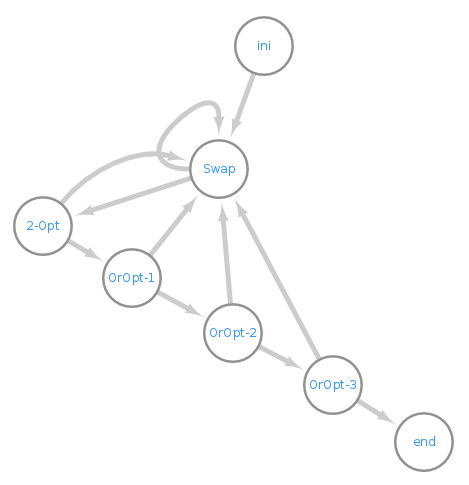
\includegraphics[scale=0.5]{figuras/rvnd/RVND_dataflow_nomes.png}}
    \caption{Arquitetura simplificada do dataflow para o RVND com as vizinhanças utilizadas.}
    \label{fig:rvndGraph}
\end{figure}

A implementação do nó operador (\textit{Swap, 2-Opt, OrOpt-1, OrOpt-2, OrOpt-3}) é tão simples quanto o Algoritmo~\ref{alg:rvndOper} e cada estratégia de vizinhança é atrelada a um nó operador, sendo que a ordem desses é variada para cada execução do método para caracterizar o RVND, a decisão de para qual nó enviar o resultado é tomada pela configuração do dataflow.
Quando a solução atinge o nó final (\textit{end}) esta é salva e o processo termina.

\begin{algorithm}[htpb]
\caption{Nó de vizinhança do RVND}
\label{alg:rvndOper}
\begin{algorithmic}[1]
    \Function{RVND\_Oper}{Solução: $s$}
        \Let{$s'$}{melhor solução de $N^k(s)$}
        \Let{$improvFlag$}{$f(s') < f(s)$}
        \Return{$(s', improvFlag)$}
    \EndFunction
\end{algorithmic}
\end{algorithm}

Pode ser visto destacado na Figura~\ref{fig:rvndGraphDestacado} uma vizinhança com suas ligações ao grafo dataflow, uma de entrada de dados e duas outras de saída que são para o caso de haver ou não uma melhoria no valor da solução.
Para acoplar uma nova vizinhança ao algoritmo basta que seja inserido um novo nó de enumeração com sua entrada de dados vindo do nó anterior e duas saídas de dados, uma retornando para a primeira vizinhança e outra para a vizinhança seguinte, conforme destacado na mesma figura.

\begin{figure}[htbp]
    \centerline{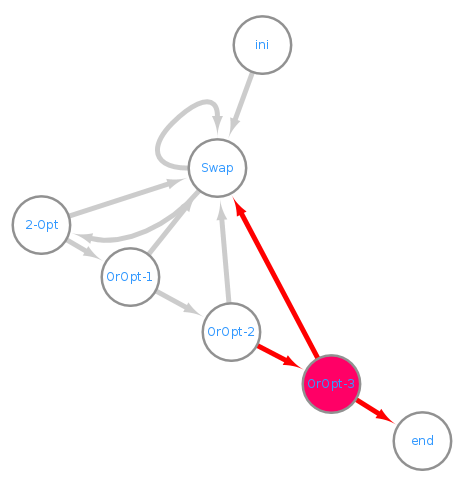
\includegraphics[scale=0.5]{figuras/rvnd/RVND_dataflow_nomesDestacado.png}}
    \caption{Uma vizinhança e suas ligações ao grafo dataflow no RVND.}
    \label{fig:rvndGraphDestacado}
\end{figure}

\subsection{Passo iterativo}

Utilizando o termo convencionado na seção~\ref{subsec:passoIterativo}, cada passo iterativo do RVND retorna a melhor solução encontrada para a vizinhança atual.
Assim sendo $N^k$ a vizinhança atual temos o passo iterativo para o RVND expresso na Equação~\ref{eq:rvndPassoIterativo}.
\begin{equation} \label{eq:rvndPassoIterativo}
    \rho^{RVND}(s) = s' \in N^k \quad \textrm{sendo} \quad f(s') < f(s''), \forall s'' \in N^k(s) \land s'' \ne s
\end{equation}
Fazendo uso da notação de movimentos temos podemos escrever \ref{eq:rvndPassoIterativo} como a Equação~\ref{eq:rvndPassoIterativoMovimento}.
\begin{equation} \label{eq:rvndPassoIterativoMovimento}
    \rho^{RVND}(s) = m \circ s \quad \textrm{com} \quad m \in M^k \land \widehat{m} < \widehat{m_i} \mid \forall m_i \in M^k
\end{equation}

\section{DVND}\label{subsec:dvnd}

Foi descrito na Seção~\ref{sec:dvndClassico} o algoritmo do DVND, contudo um modelo dataflow para o DVND pode ser visto na Figura\ref{fig:dvndGraph}, o método usa $P + 1$ nós iniciais (\textit{ini0}, \textit{ini1}, \dots \textit{iniP}) que alimentam os nós operadores (\textit{Swap, 2-Opt, OrOpt-1, OrOpt-2, OrOpt-3}) e o nó gerente (\textit{man}) com a solução inicial para a busca local.

\begin{figure}[htbp]
    \centerline{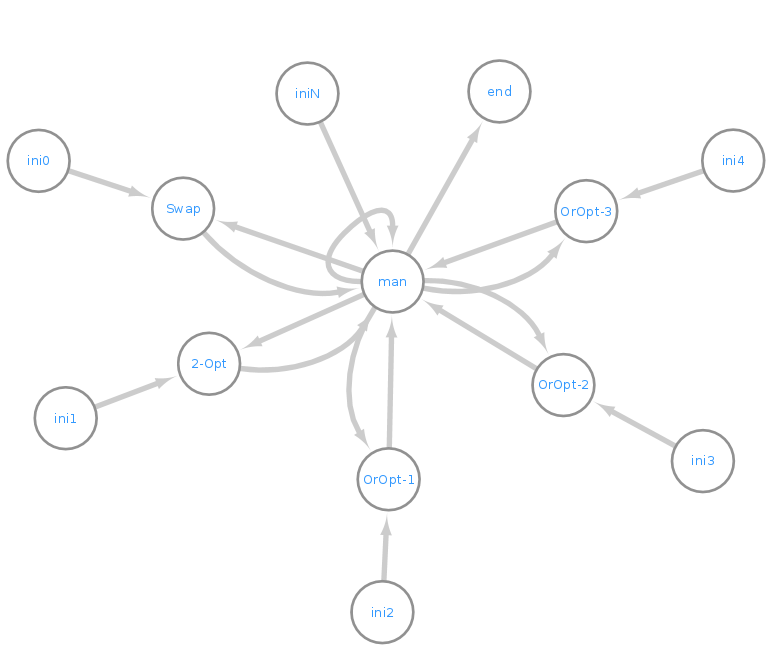
\includegraphics[scale=0.6]{figuras/dvnd/DVND_dataflow_nomes.png}}
    \caption{Arquitetura simplificada do dataflow para o DVND com as vizinhanças utilizadas.}
    \label{fig:dvndGraph}
\end{figure}

Cada nó operador utiliza uma estratégia de vizinhança diferente, quando termina de enumerar as soluções este retorna a melhor para o nó gerente que mantém a melhor solução encontrada até o momento.
Então o nó gerente identifica a melhor solução conhecida e a envia de volta para o dataflow (como no Algoritmo.~\ref{alg:dvndMan}) que encaminha a solução para todos os nós operadores parados, o processo se repete até que nenhum nó operador encontre uma solução melhor.
Então a melhor solução encontrada é enviada para o nó final (\textit{end}) que salva o resultado da busca local.

\begin{algorithm}[htpb]
\caption{Nó \textit{man} do DVND}
\label{alg:dvndMan}
\begin{algorithmic}[1]
    \Function{DVND\_Man}{Solução: s, Histórico: H}
        \Let{$H$}{$H \cup \{s\}$}
        \Return{$bestSolution(H)$}
    \EndFunction
\end{algorithmic}
\end{algorithm}

O critério de parada é alcançado quando nenhum nó operador consegue melhorar a solução atual significando que está corresponde a ótimo local para todas as vizinhanças usadas no processo.
Este é, de certa forma, o mesmo critério utilizado por ambos RVND e DVND, contudo o caminho percorrido pelos diferentes processos pode levar a a ótimos locais diferentes. Tanto para o RVND quanto DVND as estratégias de vizinhança são atribuídas aos nós \textit{oper} e os métodos não definem o comportamento interno destes nós facilitando sua alteração ou mesmo a adição de uma nova vizinhança.

\begin{figure}[htbp]
    \centerline{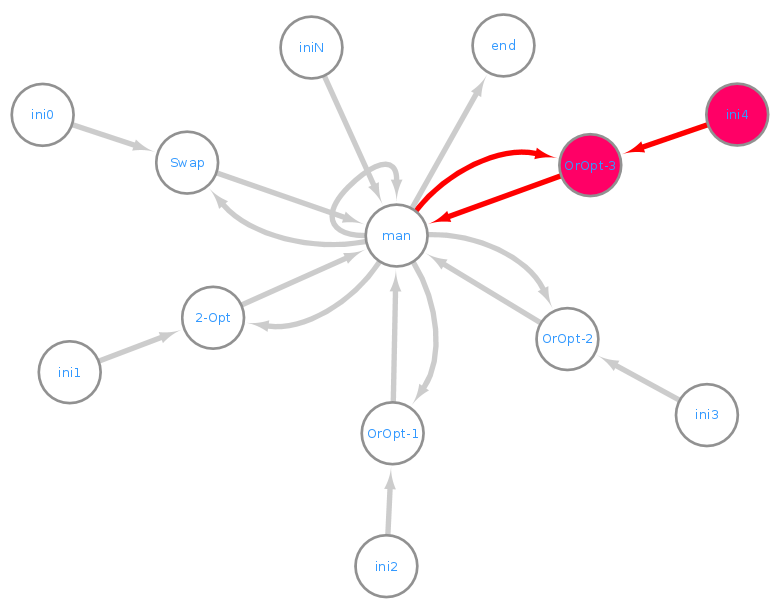
\includegraphics[scale=0.6]{figuras/dvnd/DVND_dataflow_nomesDestacado.png}}
    \caption{Uma vizinhança e suas ligações ao grafo dataflow no DVND.}
    \label{fig:dvndGraphDestacado}
\end{figure}

Como dito anteriormente, qualquer vizinhança pode ser facilmente acoplada ao procedimento apenas adicionando um novo nó operador \textit{oper} ao grafo dataflow, conforme destacado na Figura~\ref{fig:dvndGraphDestacado}, o que é uma grande característica do método, e como os nós são independentes é possível fazê-lo sem impactar nos outros nós.
Inicialmente pode parecer que muitos nós operadores podem sobrecarregar o nó gerente, mas é importante notar que o tempo computacional gasto pelos nós operadores é geralmente muito mais caro (exploração das vizinhanças é o processo mais caro de uma meta-heurística), desta forma não será um grande problema mesmo quando os nós operadores responderem em tempos curtos.

No trabalho apresentado em~\cite{df-dvnd2018} o modelo dataflow usado possuía apenas uma porta de saída então a mensagem seria enviada para todos os nós a ele vinculados, numa melhoria a esta implementação foi implementado e sugerido um aperfeiçoamento ao Sucuri para comportar portas de saída diferentes para destinos diferentes.
No modelo proposto (veja Figura~\ref{fig:dvndGraph}), o nó gerente é ligado a todos os nós operadores o que causaria uma inundação (\emph{flooding}) na rede, desta forma possuir mais de uma porta de saída permite evitar que um nó processe indevidamente uma solução ou que receba uma mensagem com uma indicação de que não deve ser processada o que causaria uma troca de mensagens desnecessária, problema esse que se intensifica ao rodar o processamento em rede.
Um problema que permanece é o escalonador centralizado, o que significa que num processamento em rede cada mensagem precisa ser enviada de volta para o computador rodando o nó gerente para só então ser enviada para o seu nó de destino, incluindo nisso as mensagens de \emph{feedback} explicadas no Sub-seção~\ref{text:flipFlop}.
Contudo a disponibilização de um escalonador distribuído demandaria um novo projeto para a o dataflow do DVND (Figura~\ref{fig:dvndGraph}) de forma a fazer melhor uso deste recurso.
Apesar das limitações atuais deste projeto em desenvolvimento, o Sucuri já provê um ambiente que pode ser facilmente escalado de uma máquina para um experimento em rede completamente distribuído.

\subsection{Passo iterativo}

Utilizando o termo convencionado na seção~\ref{subsec:passoIterativo}, cada passo iterativo do DVND retorna a melhor solução encontrada para todas as vizinhanças.
Dessa forma, sendo $N$ a união de todas as vizinhanças, o passo iterativo do DVND pode ser dado pela Equação~\ref{eq:dvndPassoIterativo}.
\begin{equation} \label{eq:dvndPassoIterativo}
\rho^{DVND}(s) = s' \in N \quad \textrm{com} \quad f(s') < f(s''), \forall s'' \in N(s) \land s'' \ne s
\end{equation}
Fazendo uso da notação de movimentos podemos escrever \ref{eq:dvndPassoIterativo} como a Equação~\ref{eq:dvndPassoIterativoMovimento}.
\begin{equation} \label{eq:dvndPassoIterativoMovimento}
\rho^{DVND}(s) = m \circ s\quad \textrm{com} \quad m \in \mathcal{M} \land \widehat{m} < \widehat{m_i} \mid \forall m_i \in \mathcal{M}
\end{equation}

Pelo passo iterativo do RVND $\rho^{RVND}$ (\ref{eq:rvndPassoIterativoMovimento}) e do DVND $\rho^{DVND}$ (\ref{eq:dvndPassoIterativoMovimento}) podemos concluir que $\rho^{DVND}(s) \le \rho^{RVND}(s)$, contudo isso não é suficiente para afirmar que o DVND encontre necessariamente melhores resultados.% pois o DVND pode acabar convergindo muito cedo para um mínimo local.

\subsection{Nó de flip flop}\label{subsec:flipFlop}

É esperado um comportamento sem estado para os nós num grafo de uma arquitetura dataflow contudo no modelo do DVND proposto (veja Figura~\ref{fig:dvndGraph}) o nó gerente precisa manter o histórico da melhor solução já encontrada até o momento e decidir se o método alcançou ou não um ótimo local. Para alcançar este comportamento, é apresentado em \cite{endm2018:araujo} um nó de flip flop \label{text:flipFlop} (nó \textit{FF} na Figura~\ref{fig:flipFlop}), este nó possui duas portas de entrada, uma que de fato recebe a informação do nó anterior e outra que o retro-alimenta com sua própria saída para manter o histórico do resultado. A intenção desse padrão é conceder ao nó a capacidade de realizar uma decisão baseada na última iteração sem necessariamente tornar o nó statefull.

\begin{figure}[htbp]
    \centerline{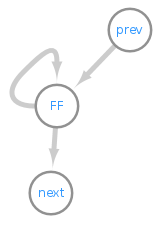
\includegraphics[scale=1.0]{figuras/dataflow/Flip_flop.png}}
    \caption{FF identifica o nó de flip flop.}
    \label{fig:flipFlop}
\end{figure}

É importante ressaltar que o nó \textit{oper0} no RVND (Figura~\ref{fig:rvndGraph}) também possui uma retroalimentação contudo não é um nó de flip flop pois não retroalimenta sua própria saída, este nó não precisa da informação de sua última execução para realizar o seu processamento, desta forma possui apenas uma porta de entrada.

\subsection{Múltiplas portas de saída}\label{subsec:multiplasSaidas}

Em modelo dataflow um nó será processado quando todas as suas dependências forem satisfeitas, contudo, ao final de seu processamento o resultado pode ser enviado como entrada para um ou mais nós.
Pode ser visto na Figura~\ref{fig:dataflowMo0} que o nó \textit{MO} está conectado a um nó com informação de entrada (nó \textit{prev}) e ligado a três nós de saída (\textit{next 0}, \textit{next 1} e \textit{next 2}).

\begin{figure}[htbp]
    \centerline{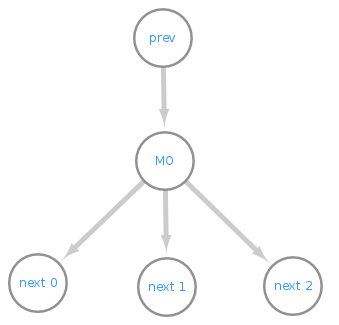
\includegraphics[scale=0.9]{figuras/dataflow/multi_output0.png}}
    \caption{Pedaço de um grafo dataflow em que o nó \textit{MO} do datalflow possui múltiplas saídas.}
    \label{fig:dataflowMo0}
\end{figure}

No modelo atual de implementação da biblioteca Sucuri é possível que um nó receba informações de vários outros nós contudo existe apenas uma porta de saída a qual podem estar conectados vários nós.

Pegando-se o exemplo da Figura~\ref{fig:dataflowMo3}, quando o nó \textit{MO} termina de processar seu resultado é enviado para a única porta de saída existente a qual estão ligados os nós \textit{next 0}, \textit{next 1} e \textit{next 2}, dessa forma todos os nós seguintes vão receber a informação e estarão aptos para processamento mesmo que a informação não seja destinada a eles.
Cada um desses nós terá então que verificar se a mensagem é destinada a ele antes de processar ou não a informação.

\begin{figure}[htbp]
    \centerline{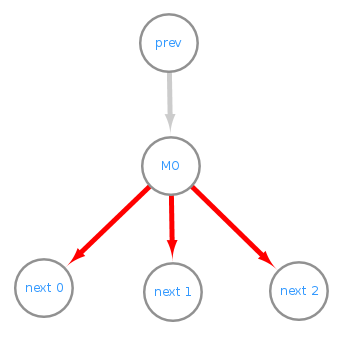
\includegraphics[scale=0.9]{figuras/dataflow/multi_output3.png}}
    \caption{Quando o nó \textit{MO} termina de processar seu resultado é enviado para todos os nós subsequentes (\textit{next 0}, \textit{next 1} e \textit{next 2}).}
    \label{fig:dataflowMo3}
\end{figure}

Foi implementada a alteração exemplificada na Figura~\ref{fig:dataflowMo1}, nesse caso existe uma porta de saída para cada nó ligado ao nó \textit{MO}, este identifica os destinatários da mensagem e aciona apenas aqueles necessários.

\begin{figure}[htbp]
    \centerline{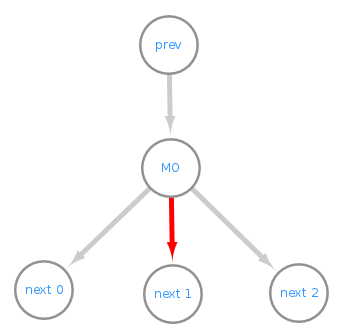
\includegraphics[scale=0.9]{figuras/dataflow/multi_output1.png}}
    \caption{Quando o nó \textit{MO} termina de processar é possível escolher qual porta de saída será utilizada e assim decidir o destino da informação.}
    \label{fig:dataflowMo1}
\end{figure}

No DVND, ao escolher o destinatário da mensagem é possível evitar uma grande quantidade de transmissões desnecessárias de mensagens, evitando assim que os nós de vizinhança sejam acionados apenas para identificar que não precisam processar a mensagem.
Vejamos, por exemplo, o nó \textit{man} da Figura~\ref{fig:dvndGraph} sem o artifício de múltiplas portas de saída todas as mensagens serão enviadas para todas as 5 vizinhanças e para o nó finalizador (\textit{end}) sendo que a mensagem só é enviada para os nós ociosos naquele momento.

A implementação de múltiplas portas de saída trás vantagens ainda mais significativas quando o tamanho da mensagem a ser transmitido é grande e quando a execução do processamento está sendo feita em um ambiente de mais de uma máquina o que envolve troca de mensagens pela rede.

\section{GDVND}\label{subsec:gdvnd}

Trazendo o conceito de \textit{movimentos independentes} (discutido na Seção \ref{subsubsec:movimentosIndependentes}) para o DVND surge a ideia do \emph{Generalized Distributed Variable Neighborhood Descent} (\emph{GDVND}).
A ideia do GDVND é um DVND que trabalha no escopo de movimentos de melhora e não em melhores soluções.
No DVND, a cada iteração o método recebe uma nova solução de uma das vizinhanças e verifica qual a melhor para então enviar esta para ser processada pelas vizinhanças ociosas que ainda não a processaram, sempre mantendo a melhor solução já encontrada.
A diferença para o GDVND é que este recebe não somente uma solução mas a solução com um conjunto de movimentos de melhora encontrado pela vizinhança, então o método tenta combinar os movimentos da melhor solução atual com aqueles da solução recebida.
Para tanto é necessário que as soluções tenham a mesma solução base, então é necessário identificar o conjunto de movimentos independentes que proporcione o maior ganho em termos de valor da solução.
Além de melhorar a solução a utilização da composição de movimentos proporciona uma melhor utilização dos recursos usados no processamento ao aproveitar computações realizadas em nós diferentes.

O grafo dataflow do GDVND é equivalente ao do DVND expresso na Figura~\ref{fig:dvndGraph} alterando apenas a informação trafegada entre os nós e a implementação interna do nó gerenciador, conforme Algoritmo~\ref{alg:gdvndMan}, ao qual caberá combinar os movimentos de vizinhanças diferentes.
Na linha \ref{alg:gdvndMan:merge} é chamado o processo combinar movimentos que pode ser visto em mais detalhes no Algoritmo~\ref{alg:gdvndMergeFunc}.
Os movimentos são combinados para formar uma solução resultante, tomando proveito do Teorema da independência de movimentos dois a dois (Teorema~\ref{teo:independenciaMovimentos2a2}) o valor da solução resultante pode ser calculado para dois movimentos, sem a necessidade de recalcular toda a solução, o que é particularmente útil para grandes instâncias e problemas cujo cálculo da função objetivo é muito caro computacionalmente.
Pode-se utilizar o mesmo teorema para estimar o valor das soluções na composição de mais de dois movimentos dois a dois.

\begin{algorithm}[htpb]
\caption{Nó \textit{man} do GDVND}
\label{alg:gdvndMan}
\begin{algorithmic}[1]
    \Function{GDVND\_Man}{Solução: $s$, Histórico: $H$, Vizinhança: $k$}
        \Let{$s_{merged}$}{$GDVND\_merge(s, bestSolution(H))$} \label{alg:gdvndMan:merge} \Comment{Combina a solução atual com a melhor conhecida}
        \Let{$H(k)$}{$min(s, s_{merged}, bestSolution(H))$} \Comment{Atualiza o histórico da vizinhança $k$ com a melhor solução}
        \Return{SoluçãoBase($H(k)$), Movimentos($H(k)$)}
    \EndFunction
\end{algorithmic}
\end{algorithm}

Seja um grafo $G = (V, E)$ cujos vértices $V$ são movimentos e as arestas $E$ indicam se um movimento é independente de outro.
Dessa forma encontrar o melhor sub-conjunto de movimentos independentes entre si dois a dois corresponderia a encontrar o sub-grafo completo correspondente ao clique maximal em que o o somatório do valor dos vértices seja máximo.

Neste trabalho é usada uma heurística para encontrar o melhor sub-conjunto de movimentos independentes, o Algoritmo~\ref{alg:gdvndMergeFunc} ilustra a heurística utilizada para fazer o \emph{merge} dos movimentos da solução.
O método apenas pode ser executado quando as soluções base são iguais para as duas soluções de entrada.
Os movimentos são reunidos num conjunto $M'$ e então ordenados conforme a melhoria que podem aplicar à solução.
Em seguida cada movimento é testado, em busca de conflitos, contra as demais movimentos, caso haja conflito este movimento é descartado, os movimentos foram dispostos de forma que os movimentos com pior resultado sobre a solução sejam testados primeiro, desta forma aqueles com melhores valores são deixados por último para que possam ser preservados caso possuam conflitos com algum outro.

\begin{algorithm}[htpb]
\caption{Combinando movimentos de soluções diferentes}
\label{alg:gdvndMergeFunc}
\begin{algorithmic}[1]
    \Function{GDVND\_merge}{Solução: $s_1$, Solução: $s_2$}
        \If{SoluçãoBase($s_1$) = SoluçãoBase($s_2$)} \Comment{Somente soluções com a mesma solução base podem ser combinadas}
            \Let{$M'$}{sorted(Movimentos($s_1$) $\cup$ Movimentos($s_2$))} \Comment{Movimentos ordenados pelo valor da melhoria na solução}
            \For{$i \gets 0$ to $len(M')$}
                \For{$j \gets (i + 1)$ to $len(M')$}
                    \If{$m_i \nparallel m_j$}
                        \Let{$M'$}{$M' - {m_i}$}
                        \State break
                    \EndIf
                \EndFor
            \EndFor
            \Return{SoluçãoBase($s_1$), $M'$}
        \EndIf
        \Return{$min(s_1, s_2)$}
    \EndFunction
\end{algorithmic}
\end{algorithm}

O retorno da iteração de cada vizinhança do GDVND passa a corresponder não a uma solução $s'$ mas a uma tupla com a solução e os movimentos aplicados, assim temos a resposta como $(s', \{m_1^x, m_2^x, \dots, m_k^x\})$.

É importante ressaltar a diferença do \emph{Multi Improvement} para o GDVND, o primeiro é uma estratégia de exploração de vizinhanças em que a busca local avança de uma solução para outra fazendo uso de uma composição de movimentos independentes $\{m_1^x, m_2^x, \dots, m_k^x\} \subset M^x$ pertencentes a uma vizinhança, no caso do GDVND os movimentos independentes são oriundos de todas as vizinhanças utilizadas pelo algoritmo.
Ainda na analogia com o \emph{Multi Improvement}, o GDVND poderia ser visto como um \emph{multi improvement} em que a sua vizinhança é a união de todas as vizinhanças utilizadas no GDVND.

A mesma ideia pode ser aplicada para um conjunto de movimentos $M = \{ m_1, m_2, m_3, ...\}$, ditos independentes se para uma solução $s$ qualquer e para todo subconjunto não-vazio $M' = \{ m_1, m_2, m_3, ..., m_k \} \subseteq M$ temos $\widehat{m_1}(s) + \widehat{m_2}(s) + \widehat{m_3}(s) + ... + \widehat{m_k}(s) = \widehat{m_1}(m_2 \circ m_3 \circ ...\circ m_k \circ s)$. 
Utilizaremos a letra $I$ para denotar movimentos independentes, por exemplo, $I(\{m_3, m_5, m_9\})$.

\subsection{Detecção movimentos independentes} \label{subsec:gdvndDetectarMovimentosIndependentes}

Para detectar quais movimentos são independentes, uma estrutura de dados $C$ para gerenciamento de conflitos foi proposta.
No caso do problema em questão, a estrutura se trata de vetor com $N$ bits, onde cada bit $i$ indica se houve alguma alteração relativa ao cliente $i$.

Exemplo $C: |0|0|0|1|1|1|1|0|0|0|0|0|0|$

Assim, a estrutura $C$ começa com todos bits zero, considerando uma solução de referência $s$.
Cada movimento altera a estrutura $C$ além de alterar a solução corrente, indicando quais posições estão comprometidas.
Da mesma maneira, uma função $d$ de detecção de conflitos indica se um movimento é "aplicável" dada certa configuração da estrutura de conflitos.

Dessa forma, ao aplicar um movimento, se for necessário alterar um bit para 1 que já tenha valor 1 então o movimento atual é conflitante com o anterior ou algum dos anteriores.

Como podemos ver a seguir a detecção de conflitos para uma solução de tamanho $n=13$, os movimentos $Swap_{1,3} \parallel Swap_{5,9}$, $Swap_{5,9} \parallel Swap_{3,7}$ mas $Swap_{1,3} \nparallel Swap_{3,7}$.\\
$C:$ |0|\textbf{0}|0|\textbf{0}|0|0|0|0|0|0|0|0|0| - $Swap_{1,3}$ \\
$C:$ |0|1|0|1|0|\textbf{0}|0|0|0|\textbf{0}|0|0|0| - $Swap_{5,9}$ \\
$C:$ |0|1|0|\textbf{1}|0|1|0|\textbf{0}|0|1|0|0|0| - $Swap_{3,7}$ \\
$C:$ |0|1|0|\textcolor{red}{0}|0|1|0|1|0|1|0|0|0| - Conflito \\
A estrutura começa com todos os bits com valor zero, os bits em negrito indicam aqueles que serão alterados pelo movimento atual, na última linha o bit em vermelho indica a existência de um conflito ($Swap_{1,3} \nparallel Swap_{3,7}$).

\subsection{Exemplo de execução} \label{subsec:gdvndExemplo}

No DVND, várias buscas começam de uma mesma solução de referência e o melhor movimento (ou primeiro de melhora) é retornado como candidato à inclusão em um pool de movimentos, chamado Histórico.
Este pool pode ser visto como um grafo não direcionado, no qual os vértices são movimentos e arestas indicam conflitos entre movimentos.
Porém, setas especiais são utilizadas para marcar dependência entre movimentos. Se $m_B$ depende de $m_A$, então $m_B$ só pode ser aplicado se $m_A$ for aplicado antes na solução.
Escolhendo o maior (ou menor) conjunto independente neste grafo, respeitando os conflitos e dependências, resultará na melhor combinação de movimentos em um dado momento, considerando múltiplas estruturas de vizinhança simultaneamente.

A Figura~\ref{fig:exemplo-dvnd} apresenta um exemplo do grafo de Histórico para uma execução do GDVND com três processos de busca.

\begin{figure}[htpb]
    \centering
    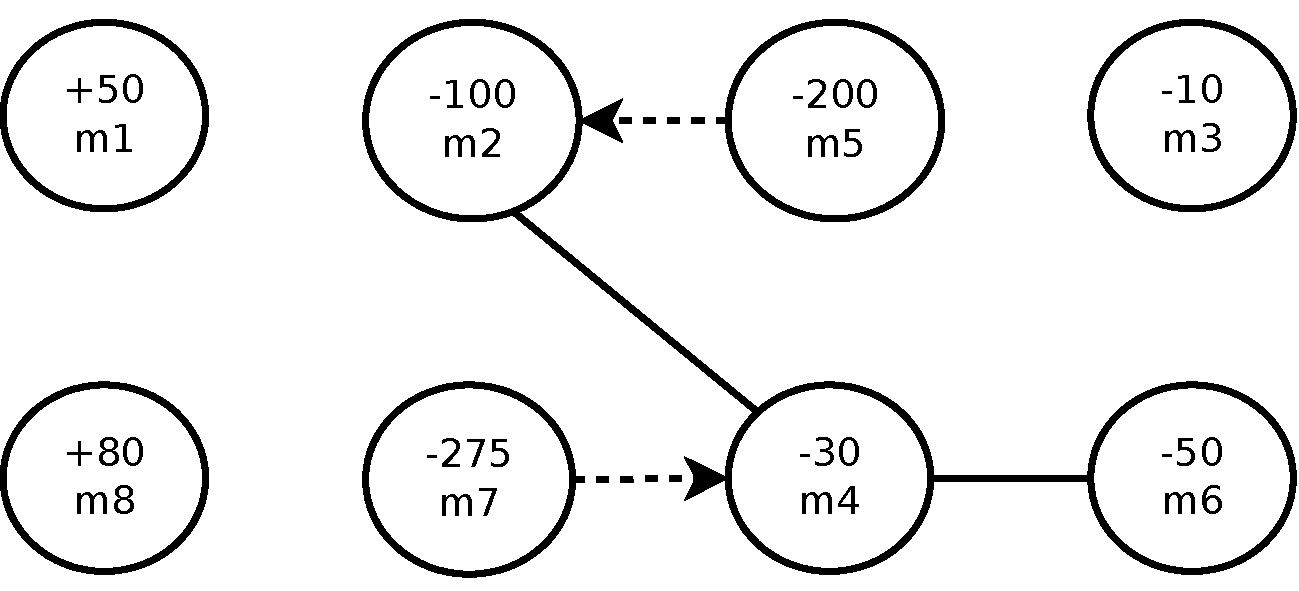
\includegraphics[width=0.65\linewidth]{figuras/gdvnd/dvnd_exemp.pdf}
    \caption{Exemplo de um grafo de Histórico.
    A combinação ótima de custos consiste nos movimentos $m_2$, $m_3$, $m_5$ e $m_6$.
    \label{fig:exemplo-dvnd}}
\end{figure}

Para entender melhor a ideia do algoritmo, a tabela abaixo simula a execução do algoritmo para três processos.

\begin{table}[htpb]
\centering
\caption{Execução do GDVND}
\begin{tabular}{|c|cccc|c|}
\hline
    \# & $f$ & solução & direção & processo & conflito\\\hline
    1  & 1000 & $s_1$ & $\rightarrow$ & P1 &\\
    2  & 1000 & $s_1$ & $\rightarrow$ & P2 &\\
    3  & 1000 & $s_1$ & $\rightarrow$ & P3 &\\\hline
    4  & 970 & $m_4 \circ s_1$ & $\leftarrow$ & P3 &\\
    5  & 970 & $m_4 \circ s_1$ & $\rightarrow$ & P3 &\\\hline
    6  & 900 & $m_2 \circ s_1$ & $\leftarrow$ & P1 & \\
    7*  & 900 & $m_2 \circ s_1$ & $\rightarrow$ & P1 & $m_2 \nparallel m_4$\\\hline
    8  & 1050 & $m_1 \circ s_1$ & $\leftarrow$ & P2 &\\
    9*  & 900 & $m_2 \circ s_1$ & $\rightarrow$ & P2 &\\\hline
    10 & 890 & $m_3 \circ m_2 \circ s_1$ & $\leftarrow$ & P1 & \\
    11 & 890 & $m_3 \circ m_2 \circ s_1$ & $\rightarrow$ & P1 & $m_2 \parallel m_3$\\\hline
    12 & 700 & $m_5 \circ m_2 \circ s_1$ & $\leftarrow$ & P2 &\\
    13 & 690 & $m_5 \circ m_3 \circ m_2 \circ s_1$ & $\rightarrow$ & P2 & $m_3 \parallel m_5$ e $m_2 \parallel m_5$\\\hline
    14 & 695 & $m_7 \circ m_4 \circ s_1$ & $\leftarrow$ & P3 &\\
    15 & 685 & $m_7 \circ m_4 \circ m_3 \circ s_1$ & $\rightarrow$ & P3 & $m_2 \nparallel m_7$ e $m_5 \nparallel m_4$\\\hline
    16 & 840 & $m_6 \circ m_3 \circ m_2 \circ s_1$ & $\leftarrow$ & P1 &\\
    17 & 640 & $m_6 \circ m_3 \circ m_5 \circ m_2 \circ s_1$ & $\rightarrow$ & P1 & $m_6 \parallel m_2, m_3, m_5$\\\hline
    18 & 765 & $m_8 \circ m_7 \circ m_4 \circ m_3 \circ s_1$ & $\leftarrow$ & P3 &\\
    19 & 640 & $m_6 \circ m_3 \circ m_5 \circ m_2 \circ s_1$ & $\rightarrow$ & P3 & $m_8 \nparallel m_6$\\\hline
\end{tabular}
\end{table}

O Histórico começa distribuindo a solução $s_1$ para cada busca, e eventualmente coleta um novo movimento e distribui uma nova solução.
Todos os cálculos são feitos sobre uma mesma solução de referência $s_1$, que só é modificada no passo 20 do algoritmo.
Nas iterações 7 e 9, note que existem conflitos a serem resolvidos (vide grafo na Figura~\ref{fig:exemplo-dvnd}).
Após a iteração 19, o Histórico percebe que os três processos tem movimentos em comum: $m_3$, $m_5$ e $m_2$. Então uma nova solução $s_2$ é armazenada no Histórico como solução de referência, sendo ela $s_2 = m_3 \circ m_5 \circ m_2 \circ s_1$ (de custo 690).
Assim, os processos P1 e P3 continuam naturalmente processando a solução $m_6 \circ s_2$ (antiga $m_6 \circ m_3 \circ m_5 \circ m_2 \circ s_1$), e P2 continua com $s_2$ (antiga $m_5 \circ m_3 \circ m_2 \circ s_1$).
Note também que, ao adotar estes três movimentos, todos movimentos com conflitos (ou dependência de algum movimento em conflito) tem de ser eliminados. Então, $m_4$ e $m_7$ são descartados.
Vale observar que $m_1$ e $m_8$ nunca foram armazenados, pois eram de piora.
O grafo final então consiste somente dos movimentos $m_6$, $m_3$, $m_5$ e $m_2$.

%OBSERVAÇÃO IMPORTANTE: eu acho que este processo pode ser mais estável se a unificação ocorrer após UMA iteração que o conjunto de movimentos comuns se mantenha estável, mas teremos que experimentar para saber =D

\begin{table}[htpb]
\centering
\caption{Consolidação de uma nova solução no GDVND}
\begin{tabular}{|c|ccc|}
\hline
\# & $f$ & solução & local\\\hline
20 & 690 & $s_2 = m_3 \circ m_5 \circ m_2 \circ s_1$ &  Histórico\\
   & 640 & $m_6 \circ s_2$ & P1\\
   & 690 & $s_2$           & P2\\
   & 640 & $m_6 \circ s_2$ & P3\\\hline
\end{tabular}
\end{table}

\subsection{Controle de execução entre CPU e GPU}

Para entender como o método tira proveito da arquitetura híbrida CPU-GPU segue o presente exemplo:
A CPU é utilizada para decidir qual solução cada processo de busca local irá utilizar, minimizando as transferências de memória CPU-GPU. % e, assim, maximizando o aproveitamento na estrutura de dados ADS (informações auxiliares usada para acelerar o cálculo do valor da solução) das na memória da GPU.

EXEMPLO:\\
 Processo A $\rightarrow$ CPU\\
 Processo B $\rightarrow$ Kernel GPU Swap\\
 Processo C $\rightarrow$ Kernel GPU 2-Opt\\
 Processo D $\rightarrow$ Kernel GPU Or-1\\
 Processo E $\rightarrow$ Kernel GPU Or-2\\
 Processo F $\rightarrow$ Kernel GPU Or-3

Solução $s_1$ = [1,2,3,4,5,6,7,8,9,10], ($f(s_1) = 1000$).

A solução $s_1$ entra na GPU para todas as buscas B-F, cada uma em um fluxo (\emph{thread}) distinto.
Supomos que o processo B (Swap) termina antes com ganho -100 (melhora, $\widehat{m_1} = -100$) na troca $m_1 = Swap_{2,5}$.
A CPU então cria $s_2 = m_1 \circ s_1$.
Como $s_2$ é a melhor solução atual, ela é copiada para a GPU, e o processo B roda em cima de $s_2$ = [1,5,3,4,2,6,7,8,9,10], com $f(s_2) = 900$.

Neste momento, o processo D termina com $m_2 = Or-1_{7,9}$, movendo cliente 7 para depois do 9, com ganho -50, $\widehat{m_2} = -50$.
A CPU então analisa $m_1$ e $m_2$, como não há conflitos uma solução $s_3 = m_2 \circ m_1 s_1$ é criada para o processo D executar. $s_3$=[1,5,3,4,2,6,8,9,7,10], com $f(s_3) = 850$

O processo C termina com o movimento $m_3=2Opt_{1,3}$ (inverte de 1 a 3) com ganho -120 ($\widehat{m_3} = -120$.
A CPU percebe que $m_3 \nparallel m_1$, mas $m_3 \parallel m_2$.
Então a solução $s_4= m_4 \circ m_2 \circ s_1$ é gerada e passada à GPU para o processo C, com $f(s_4) = 830$

O processo E termina sem ganho com o movimento $m_4 = Or-2_{1,4}$ (move clientes 1,2 para depois do 4).
A CPU percebe que $m_4 \nparallel m_1$ e $m_4 \nparallel m_3$ mas $m_4 \parallel m_2$.
Porém, a melhor configuração atual é $s_4$ ($f(s_4)=830$), então a busca parte dela (e ela já está na memória da GPU).

Finalmente, o processo B (Swap) termina novamente com melhora -60 e troca $m_5=Swap_{3,8}$.
Esta troca roda em cima de $s_2$, então não existem outros movimentos para haver conflito.
A solução $s_5 = m_5 \circ s_2$ com $f(s_5) = 840$ é criada, porém, a solução $s_4$ ($f(s_4) = 830$) é melhor.
A CPU então relança o processo B com a solução $s_4$.

\subsection{Passo iterativo}

Utilizando o termo convencionado na seção~\ref{subsec:passoIterativo}, cada passo iterativo do GDVND retorna a melhor solução encontrada para todas as vizinhanças combinado com a melhor solução já encontrada.
Dessa forma, sendo $N$ a união de todas as vizinhanças, contudo a resposta do GDVND pode conter mais de um movimento combinados simultaneamente, assim convencionaremos chamar de $\mathcal{N} = \{ m_1 \circ m_2 \circ \dots \circ m_z \circ s \mid \forall m_i \in \mathcal{M} \land \forall i, j \quad m_i \parallel m_j \}$, podemos ver, pela definição de $\mathcal{N}$, que $N \subset \mathcal{N}$ pois qualquer elemento de $N$ pode ser escrito da forma $m_1 \circ s$ que também pertence a $\mathcal{N}$.
Assim o passo iterativo do GDVND pode ser dado pela Equação~\ref{eq:gdvndPassoIterativo}.

\begin{equation} \label{eq:gdvndPassoIterativo}
\rho^{GDVND}(s) = s' \in \mathcal{N} \  \textrm{sendo} \  f(s') < f(s''), \forall s'' \in \mathcal{N}(s) \  \textrm{com} \  s'' \ne s
\end{equation}

Fazendo uso da notação de movimentos podemos escrever \ref{eq:dvndPassoIterativo} como a Equação~\ref{eq:dvndPassoIterativoMovimento}.

\begin{equation} \label{eq:gdvndPassoIterativoMovimento}
\rho^{GDVND}(s) = m_1 \circ m_2 \circ \dots \circ m_z \circ s \  \textrm{sendo} \  m \in \mathcal{M} \land \forall i,j \quad m_i \parallel m_j \  \textrm{com} \  i \ne j
\end{equation}

Pelo passo iterativo do RVND $\rho^{RVND}$ (\ref{eq:rvndPassoIterativoMovimento}), do DVND $\rho^{DVND}$ (\ref{eq:dvndPassoIterativoMovimento}) e do GDVND $\rho^{GDVND}$ (\ref{eq:gdvndPassoIterativoMovimento}) podemos concluir que $\rho^{GDVND}(s) \le \rho^{DVND}(s) \le \rho^{RVND}(s)$, contudo novamente isso não é suficiente para afirmar que o GDVND encontre necessariamente melhores resultados pois o pode acabar convergindo muito cedo para um mínimo local.

À primeira vista pode parecer que pela vizinhança do passo iterativo do GDVND conter as vizinhanças do RVND e DVND contudo podemos ver que toda solução encontrada pelo GDVND pode ser gerada por um conjunto de operações do DVND ou RVND.

Para que uma solução produzida pelo GDVND não possa ser produzida pelo RVND ou DVND deve haver um movimento nessa solução que não seja possível encontrar com RVND ou DVND, suponhamos então que o GDVND produziu uma solução $m_1 \circ m_2 \circ \dots \circ m_z \circ s \in \mathcal{N}$ com $m_i \in \{ m_1, m_2, \dots, m_z \}$ tal que $m_i \notin \mathcal{M}$.
\begin{proof}
\begin{align*}
\rho^{GDVND}(s) =& m_1 \circ m_2 \circ \dots \circ m_i \circ \dots \circ m_z \circ s & \textrm{Por comutatividade} \\
\rho^{GDVND}(s) =& m_i \circ m_1 \circ m_2 \circ \dots \circ m_z \circ s & \textrm{Fazendo } s' = m_1 \circ m_2 \circ \dots \circ m_z \circ s \\
\rho^{GDVND}(s) =& m_i \circ s' & \textrm{Logo uma contradição } \bot \\
\end{align*}
\end{proof}
Quando se escreve $\rho^{GDVND}(s) = m_i \circ s'$ chega-se a uma contradição pois, pela definição do passo iterativo do GDVND, temos que o movimento $m_i$ deveria pertencer ao conjunto $\mathcal{M}$ contudo supôs-se por hipótese que $m_i \notin \mathcal{M}$.

\section{Vizinhanças}\label{sec:neighborhoods}

% Vizinhanças Swap, 2-opt, 1-OrOpt, 2-OrOpt, 3-OrOpt
RVND, DVND e GDVND usam um conjunto de vizinhanças para processar a solução, foram escolhidas 5 estruturas diferentes, a saber, Swap, 2-Opt, OrOpt-1, OrOpt-2 e OrOpt-3, as mesmas utilizadas em~\cite{wamca2016}.
% Nesse caso o DVND pode, potencialmente, demandar 5 vezes o tempo computacional necessário pelo RVND no pior cenário (quando a exploração do RVND é ótima) pois no RVND cada solução é propagada para apenas uma vizinhança quando não é encontrada uma melhora.
No caso do DVND, a cada nova solução encontrada esta pode ser submetida para todas as vizinhanças simultaneamente (tentando explorar melhorias de vizinhanças diferentes simultaneamente).
% O desafio para melhorar o DVND frente ao RVND é explorar as vizinhanças e combinar os movimentos, de modo a evitar a geração desnecessária de soluções que causariam um desperdício de recursos computacionais.
% This idea will still be expanded in future works, as for now we lack the capability to combine moves from different neighborhoods, so it is expected to have DVND consuming bigger computational times than RVND.
A intenção principal é prover uma implementação dataflow de um procedimento de busca local de muitas vizinhanças, o que é uma contribuição original para ambas comunidades, de otimização e computação paralela.

Para a busca local foi usado uma abordagem \emph{Multi Improvement} (\emph{MI})~\cite{wamca2016} em todas as vizinhanças, na qual é calculado os custos de todos os movimentos e os resultados armazenados num vetor.
Usando a estratégia \emph{Best Improvement} (\emph{BI}) apenas a melhor solução é selecionada, na estratégia \emph{Multi Improvement} todos os \textit{movimentos independentes} são simultaneamente aplicados para a solução dada, provendo assim uma convergência mais rápida para o ótimo local.

A enumeração de todos as estratégias de vizinhança roda numa implementação em GPU, assim temos um algoritmo dataflow onde a implementação de cada nó \textit{oper} roda em GPU para ambos os casos, a configuração do lançamento do \emph{kernel} para cada estratégia de vizinhança é descrita na Tabela~\ref{tab:neighborhoodsLaunchConfigurarion}, estas configurações foram obtidas fazendo-se uso das bibliotecas fornecidas pela NVIDIA para otimização do uso dos recursos conforme o \emph{kernel} que se deseja executar, conforme descrito em~\cite{cudaProTipOccupancy}
Mais detalhes sobre a implementação GPU da enumeração das vizinhanças podem ser encontrados em \cite{wamca2016}.

% Aqui eu coloquei essa informação porque o revisor pediu, mas devo colcocar como obtenho cada configuração?

\begin{table}[ht]
\centering
\caption{Configuração de lançamento para os kernels das vizinhanças.
Onde \textit{Grid} refere-se a quantidade de grides usada, \textit{Block} o tamanho de cada bloco de threads e \textit{Shared} indica a quantidade de memória compartilhada utilizada pelas threads em cada bloco.}
\label{tab:neighborhoodsLaunchConfigurarion}
\begin{tabular}{llllllll}
\hline
\hline
\textbf{Instância} & \textbf{n} & \textbf{Vizinhança} & \textbf{Grid} & \textbf{Block} & \textbf{Shared} \\ \hline
\multirow{5}{*}{\#0 \rotatebox[origin=c]{90}{berlin52}} & \multirow{5}{*}{52} & Swap         & 26      & 53      & 1060   \\
                            & &  2-Opt        & 27      & 53      & 1060   \\
                            & & OrOpt-1      & 50      & 53      & 1060   \\
                            & & OrOpt-2      & 49      & 53      & 1060   \\ 
                            & & OrOpt-3      & 48      & 53      & 1060   \\ \hline
\multirow{5}{*}{\#1 \rotatebox[origin=c]{90}{kroD100}} & \multirow{5}{*}{100} & Swap         & 50      & 101      & 2020   \\
                            & & 2-Opt        & 51      & 101      & 2020   \\
                            & & OrOpt-1      & 98      & 101      & 2020   \\
                            & & OrOpt-2      & 97      & 101      & 2020   \\ 
                            & & OrOpt-3      & 96      & 101      & 2020   \\ \hline
\multirow{5}{*}{\#2 \rotatebox[origin=c]{90}{pr226}} & \multirow{5}{*}{226} & Swap         & 113      & 224      & 4540   \\
                            & & 2-Opt        & 114      & 224      & 4540   \\
                            & & OrOpt-1      & 224      & 224      & 4540   \\
                            & & OrOpt-2      & 223      & 224      & 4540   \\ 
                            & & OrOpt-3      & 222      & 224      & 4540   \\ \hline
\multirow{5}{*}{\#3 \rotatebox[origin=c]{90}{lin318}} & \multirow{5}{*}{318} & Swap         & 159      & 256      & 6380   \\
                            & & 2-Opt        & 160      & 256      & 6380   \\
                            & & OrOpt-1      & 316      & 256      & 6380   \\
                            & & OrOpt-2      & 315      & 256      & 6380   \\ 
                            & & OrOpt-3      & 314      & 256      & 6380   \\ \hline
\multirow{5}{*}{\#4 \rotatebox[origin=c]{90}{TRP-S500-R1}} & \multirow{5}{*}{501} & Swap         & 250      & 502      & 10040   \\
                            & & 2-Opt        & 251      & 502      & 10040   \\
                            & & OrOpt-1      & 499      & 502      & 10040   \\
                            & & OrOpt-2      & 498      & 502      & 10040   \\ 
                            & & OrOpt-3      & 497      & 502      & 10040   \\ \hline
\multirow{5}{*}{\#5 \rotatebox[origin=c]{90}{d657}} & \multirow{5}{*}{657} & Swap         & 328      & 512      & 13160   \\
                            & & 2-Opt        & 329      & 512      & 13160   \\
                            & & OrOpt-1      & 655      & 512      & 13160   \\
                            & & OrOpt-2      & 654      & 512      & 13160   \\ 
                            & & OrOpt-3      & 653      & 512      & 13160   \\ \hline
\multirow{5}{*}{\#6 \rotatebox[origin=c]{90}{rat784}} & \multirow{5}{*}{783} & Swap         & 391      & 672      & 15680   \\
                            & & 2-Opt        & 392      & 672      & 15680   \\
                            & & OrOpt-1      & 781      & 672      & 15680   \\
                            & & OrOpt-2      & 780      & 672      & 15680   \\ 
                            & & OrOpt-3      & 779      & 672      & 15680   \\ \hline
\multirow{6}{*}{\#7 \rotatebox[origin=c]{90}{TRP-S1000-R1}} & \multirow{5}{*}{1001} & Swap         & 500      & 1002      & 20040   \\
                            & & 2-Opt        & 501      & 1002      & 20040   \\
                            & & OrOpt-1      & 999      & 1002      & 20040   \\
                            & & OrOpt-2      & 998      & 1002      & 20040   \\ 
                            & & OrOpt-3      & 997      & 1002      & 20040   \\
                            & &              &          &           &    \\
\hline
\end{tabular}
\end{table}

\subsection{Tabela de conflitos}

Para classificação de movimentos independentes é necessário identificar quando um movimento aplicado a uma solução não conflita com outro movimento aplicado a mesma solução, conforme a definição estabelecida na Seção~\ref{subsubsec:movimentosIndependentes}.

A identificação de conflitos pode ser feita em $\mathcal{O}(n)$ conforme descrito na Seção~\ref{subsec:gdvndDetectarMovimentosIndependentes}, contudo nos termos deste trabalho que trata do Problema da Mínima Latência (conforme descrito na Seção~\ref{sec:mlp}), para as vizinhanças \textit{swap}, \textit{2-opt} e \textit{oropt-k} utilizadas, dois movimentos são independentes quando são satisfeitas as condições expressas na Tabela~\ref{tab_confict}, desta forma é possível identificar a a independência de movimentos em $\mathcal{O}(1)$ independente da solução base considerada.

\begin{table}[htpb]
    \small
    \centering
    \begin{tabular}{c|c|c|c}
                          & $\mbf{swap(i_2,j_2)}$             & $\mbf{2-opt(i_2,j_2)}$    & $\mbf{oropt-k_2(i_2,j_2)}$ \\
        \hline
        %\multirow{4}{*}{\mbf$swap(i_1,j_1)$}    
                          & $(|i_1-i_2| > 1) \land$         & $[(i_1 < i_2-1) \lor$     & $(j_1 < \min(i_2,j_2)-1)\,\,\, \lor  $ \\
		$\mbf{swap}$        & $(|i_1-j_2| > 1) \land$  		& $ (i_1 > j_2-1)] \land$   & $(i_1 > \max(i_2,j_2)+k_2) \lor  $ \\
		$\mbf{(i_1,j_1)}$   & $(|j_1-i_2| > 1) \land$  		& $[(j_1 < i_2-1) \lor$     & $[(i_1 < \min(i_2,j_2)-1)\,\,\, \land $ \\
			              & $(|j_1-j_2| > 1) \,\,\,$ 		& $ (j_1 > j_2+1)]\,\,\,\,$ & $\,\,\,(j_1 > \max(i_2,j_2)+k_2)] \,\,\,$ \\
        \hline 
        %\multirow{4}{*}{\mbf$2$-$opt(i_1,j_1)$} 
                          & $[(i_2 < i_1-1) \lor$    		& $(j_1 < i_2 - 1) \lor$   & \\
		$\mbf{2-opt}$	  & $ (i_2 > j_1+1)] \land$  		& $(i_1 > j_2 + 1) \lor$   & $(i_1 > \max(i_2,j_2)+k_2) \lor$   \\
		$\mbf{(i_1,j_1)}$	  & $[(j_2 < i_1-1)] \lor$   		& $(j_2 > i_1 - 1) \lor$   & $(j_1 < \min(i_2,j_2)-1) \,\,\,\,$ \\
			              & $ (j_2 > j_1+1)]\,\,\,$  		& $(i_2 > j_1 + 1)\,\,\,$  & \\
        \hline
        %\multirow{4}{*}{\mbf$oropt$-$k_1(i_1,j_1)$} 
                          & $(j_2  < \min(i_1,i_2)-1)\,\,\, \lor$	    &   				                & \\
		$\mbf{oropt-k_1}$ & $(i_2  > \max(i_1,i_2)+k_1) \lor$           & $(j_2 < \min(i_1,j_1)-1) \lor$ & $[\max(i_1,j_1)+k_1 < \min(i_2,j_2)] \lor$ \\
		$\mbf{(i_1,j_1)}$	  & $[(i_2 < \min(i_1,i_2)-1)\,\,\land$   	    & $(i_2 > \max(i_1,j_1)+k_1)$  & $[\min(i_1,j_1) > \max(i_2,j_2)+k_2]\,\,\,\,$\\
			              & $\,\,\,\,(j_2  > \max(i_1,i_2)+k_1)]\,\,\,$ &    	                            &  \\
    \end{tabular}
    \caption{Tabela de movimentos independentes (não conflitantes)}
    \label{tab_confict}
\end{table}

\section{Decomposição de vizinhanças (Disaggregated Neighborhoods)} \label{subsec:metodologiaDecomposicaoVizinhancas}

Pela Figura~\ref{fig:dvndGraph} podemos perceber que o paralelismo horizontal, isto é, aquele obtido pela utilização de mais máquinas, neste método está limitado a quantidade de vizinhanças utilizadas no método DVND.
Esta limitação representa um problema pois para obter melhor utilização do paralelismo horizontal seria necessário também adicionar novas estruturas de vizinhanças, o que aumentaria o esforço computacional e não necessariamente traria ganho de performance ou na qualidade do valor da solução.

Contudo este problema pode ser facilmente solucionado pela decomposição das vizinhanças, isto é, no lugar de um nó \textit{oper} representar toda uma estrutura de vizinhança, este passa a processar uma sub-parte desta.
% Por exemplo, na Figura~\ref{fig:operadorSwap} temos uma vizinhança de tamanho $\mathcal{O}(n^2)$ em que cada elemento é trocado com todos os elementos subsequentes, conforme pode ser visto na Figura~\ref{fig:vizinhancaTrocas} cada elemento tem um grupo independente de trocas.

\begin{figure}[htbp]
    \centerline{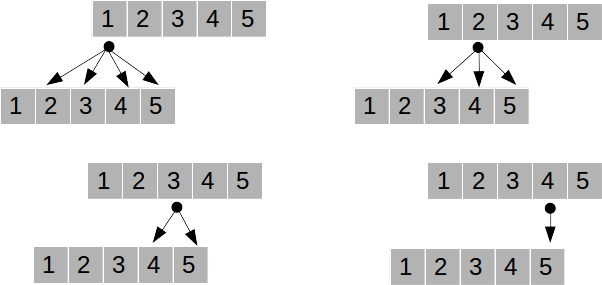
\includegraphics[scale=0.6]{figuras/vizinhanca.png}}
    \caption{Vizinhança com suas trocas para $n=5$.}
    \label{fig:vizinhancaTrocas}
\end{figure}

Isto posto, podemos separar a vizinhança em sub-grupos, um exemplo poderia ser a Figura~\ref{fig:vizinhancaTrocasDividida} que mostra a mesma vizinhança da Figura~\ref{fig:vizinhancaTrocas} dividida em dois sub-grupos. Desta forma cada sub-grupo representaria um nó \textit{oper} do diagrama dataflow DVND aumentando assim a escalabilidade horizontal do método.

\begin{figure}[htbp]
    \centerline{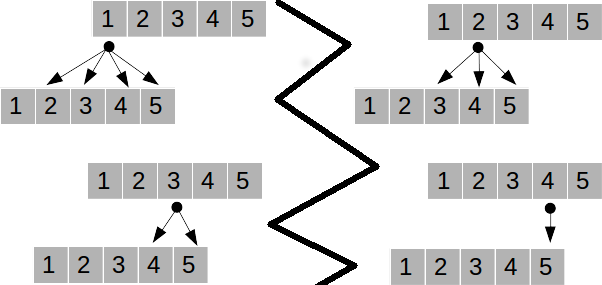
\includegraphics[scale=0.6]{figuras/vizinhancaDividida.png}}
    \caption{Vizinhança com suas trocas dividida para $n=5$.}
    \label{fig:vizinhancaTrocasDividida}
\end{figure}

A vizinhança na Figura~\ref{fig:vizinhancaTrocasDividida} exemplifica a sub-divisão em dois grupos de vizinhança contudo esta divisão limita-se apenas ao tamanho da solução proporcionando um grande potencial para o desenvolvimento do paralelismo horizontal de qualquer vizinhança sem aumentar demasiadamente o custo computacional do método.

\chapter{Resultados} \label{cap:resultados}

Este capítulo exibe os resultados computacionais dos algoritmos propostos no Capítulo~\ref{cap:metodologia} para o caso do PML, para cada instância foi gerado um conjunto com 100 soluções iniciais aleatórias que foram submetidas aos métodos para comparação dos resultados.

Quando há referência à melhoria na solução (\textit{Imp}), esta melhoria pode ser calculada pelo quociente do valor da solução inicial pela solução final, ou seja:
\begin{equation}\label{eq:calculateImprovement}
Imp = \frac{f(\textrm{solução inicial})}{f(\textrm{solução final})}
\end{equation}

Desta forma quanto maior for o valor da melhoria ($Imp$) mais o método melhorou o valor da solução inicial.

\section{Instâncias} \label{sec:instancias}

Todas as instâncias usadas nos testes computacionais e cujas configurações de lançamento foram descritas na Tabela~\ref{tab:neighborhoodsLaunchConfigurarion} são as mesmas usadas em~\cite{wamca2016}.
Para o RVND foi feita uma implementação do algoritmo clássico (Algoritmo~\ref{alg:rvnd}) e também a implementação dataflow mencionada na Figura~\ref{fig:rvndGraph} fazendo uso de uma máquina.
Para o caso do DVND foi utilizada a implementação clássica (Algoritmo~\ref{alg:dvnd}) e a implementação dataflow proposta (Figura~\ref{fig:dvndGraph}), os resultados foram obtidos com diferentes números de máquinas e os mesmos são indicados conforme o caso.

\section{Implementação e ambiente computacional}\label{sec:amb}

A implementação para cada algoritmo proposto no Capítulo~\ref{cap:metodologia} utiliza a linguagem de programação \textit{C++11} em conjunto com a API CUDA\texttrademark, para a implementação dos grafos e do ambiente dataflow foi utilizada a biblioteca Sucuri~\cite{sucuri-original}\footnote{Disponível em \url{https://github.com/tiagoaoa/Sucuri}} implementada em Python, para a integração entre o dataflow e o código CUDA foi utilizada a biblioteca SimplePyCuda~\cite{simple-pycuda}\footnote{Disponível em \url{https://github.com/igormcoelho/simple-pycuda}}. As implementações com múltiplas threads usaram a biblioteca OpenMP.
%As implementações foram compiladas através do \textit{GCC} \textit{(GNU Compiler Collection)}\footnote{O GCC está disponível no seguinte sítio eletrônico: \url{https://gcc.gnu.org/}.} com a \textit{flag} de otimização $-O3$.
O ambiente computacional utilizado em todos os testes neste trabalho consiste de 4 máquinas com a seguinte configuração:

\begin{itemize}
    \item Processador Intel\textregistered Core\texttrademark i7-4820K 3.7 GHz (4 núcleos);
    \item 8 GB de memória RAM;
    \item Sistema Operacional Ubuntu 14.10 (x64);
    \item NVIDIA GeForce GTX 780 com 2304 CUDA cores.
\end{itemize}

\newcommand{\figureDvndOrRvndDcDd}[7]{
% #1 {box, scatter}, #2 {count, imp, time}, #3 {instance number}, #4 {Tempo, Melhoria}, #5 tamanho instância, #6 {DVND, RVND}, #7 {dvnd, rvnd}
\begin{figure}%
    \centering
    \includegraphics[scale=0.9]{figuras/#7/dc_dd/#1/#7_#1100sol_#2_in#3.png}
    \caption{#4 do #6 para a instância #3 de tamanho #5. $m$ indica o número de máquinas, \textit{DC} refere-se ao #6 clássico e \textit{DD} ao #6 implementado em dataflow.}%
    \label{fig:#2_#7DcDd_in#3}%
\end{figure}
}

\newcommand{\figureDvndDcDd}[5]{
% #1 {box, scatter}, #2 {count, imp, time}, #3 {instance number}, #4 {Tempo, Melhoria}, #5 tamanho instância
    \figureDvndOrRvndDcDd{#1}{#2}{#3}{#4}{#5}{DVND}{dvnd}
}

\newcommand{\figureRvndDcDd}[5]{
% #1 {box, scatter}, #2 {count, imp, time}, #3 {instance number}, #4 {Tempo, Melhoria}, #5 tamanho instância
    \figureDvndOrRvndDcDd{#1}{#2}{#3}{#4}{#5}{RVND}{rvnd}
}

\newcommand{\tabelaEstatisticasGeral}[6]{
% #1 Descrição, #2 label, #3 {dvnd, rvnd}, #4 {DVND, RVND}, #6 DD/DC, #6 Conteúdo
\begin{table}[ht]
    \centering
    \begin{tabular}{c|ccc|cc|ccc|cc|c}
        \hline \hline
        \# & Tipo & $m$ & $n$ & $min$ & $max$ & 1Q & 2Q & 3Q & $\overline{x}$ & $\sigma$ & $p-valor$ \\ \hline
        #6
    \end{tabular}
    \caption{#1 #4 #5
        Instância (\#), tipo de implementação (Tipo), número de máquinas ($m$), tamanho da instância ($n$), valor mínimo ($min$), máximo ($max$), primeiro quartil (1Q), mediana (2Q), terceiro quartil (3Q), média ($\overline{x}$), desvio padrão ($\sigma$) e p-valor para o teste de Wilcox entre as versões (valores em negrito quando $p-valor > 0.05$).
    }
    \label{tab:#3DcDd#2}
\end{table}
}

\newcommand{\tabelaEstatisticas}[5]{
    \tabelaEstatisticasGeral{#1}{#2}{#3}{#4}{na implementação clássica (DC) e a proposta de implementação usando dataflow (DD).}{#5}
}

\newcommand{\figureDvndSogMog}[7]{
% #1 {box, scatter}, #2 {count, imp, time}, #3 {instance number}, #4 {Tempo, Melhoria}, #5 tamanho instância, #6 {DVND, RVND}, #7 {dvnd, rvnd}
\begin{figure}%
    \centering
    \includegraphics[scale=0.9]{figuras/#7/sog_mog/#1/#7_#1100sol_#2_in#3.png}
    \caption{#4 do #6 para a instância #3 de tamanho #5. \textit{SOG} refere-se a uma porta de saída e \textit{MOG} a múltiplas portas de saída.}%
    \label{fig:#2_#7SogMog_in#3}%
\end{figure}
}

\newcommand{\figureDvndGdvnd}[9]{
% #1 {box, scatter}, #2 {count, imp, time}, #3 {instance number}, #4 {Tempo, Melhoria}, #5 tamanho instância, #6 {DVND, RVND}, #7 {dvnd, rvnd}, #8 {man_time, full_time}, #9 {man, dvnd} #10 descricao
\begin{figure}%
    \centering
    \includegraphics[scale=0.9]{figuras/#7/#8/#1/#9_#1100sol_#2_in#3.png}
    \caption{#4 do #6 para a instância #3 de tamanho #5. \textit{DVND} refere-se ao tempo gasto pelo algoritmo de mesmo nome, para \textit{GDVND} é análogo ao anterior, no caso do \textit{GDVND-MAN} este se refere ao tempo do GDVND subtraido do tempo para gerenciar os movimentos.}%
    \label{fig:#2_#7_#8_in#3}%
\end{figure}
}

\newcommand{\figureDvndGdvndTime}[8]{
    \figureDvndGdvnd{#1}{#2}{#3}{#4}{#5}{#6}{#7}{man_time}{man}
}

\newcommand{\figureGdvndDvndRvnd}[9]{
% #1 {box, scatter}, #2 {count, imp, time}, #3 {instance number}, #4 {Tempo, Melhoria}, #5 tamanho instância, #6 {DVND, RVND}, #7 {dvnd, rvnd}, #8 {man_time, full_time}, #9 {man, dvnd} #10 descricao
\begin{figure}%
    \centering
    \includegraphics[scale=0.9]{figuras/#7/#8/#1/#9_#1100sol_#2_in#3.png}
    \caption{#4 do #6 para a instância #3 de tamanho #5. \textit{DVND}, \textit{GDVND} e \textit{RVND} referem-se ao tempo gasto pelos algoritmos de mesmo nome.}%
    \label{fig:#2_#7_#8_in#3}%
\end{figure}
}

% \subfloat[$m=#1$]{{ %scale=0.225
%         \includegraphics[scale=0.425]{figuras/dvnd/n#1/time#2.png}
%         \label{fig:timeDvndRvnd_n#1in#2}
%     }}%
% #1 {dvnd, rvnd, gdvnd}, #2 {sog_mog, dc_dd}, #3 {time, imp}, #4 in, #5 tamanho, #6 {box, scatter}
\newcommand{\subFig}[6]{
    \subfloat[][Instância #4, $n=#5$]{
        \includegraphics[width=.5\linewidth]{figuras/#1/#2/#6/#1_#6100sol_#3_in#4.png}
		\label{fig:#1_#2_#3_in#4}
    }
% 	\begin{subfigure}{0.45\textwidth} % dvnd_box100sol_imp_in0
% 		\includegraphics[scale=0.425]{figuras/#1/#2/#6/#1_#6100sol_#3_in#4.png}
% 		\caption{Instância #4, $n=#5$}
        % \label{fig:#1_#2_#3_in#4}
    % \end{subfigure}
}

\newcommand{\subFigBox}[5]{
	\subFig{#1}{#2}{#3}{#4}{#5}{box}
}

\newcommand{\subFigScatter}[5]{
	\subFig{#1}{#2}{#3}{#4}{#5}{scatter}
}

% #1 {dvnd, rvnd, gdvnd}, #2 {sog_mog, dc_dd}, #3 {time, imp}, #4 {box, scatter}, #5 {Tempo do DVND...}
\newcommand{\multiFigureInstanciasGeral}[5]{
	\begin{figure}[ht]
		\centering
		\subFig{#1}{#2}{#3}{0}{52}{#4}
		~
		\subFig{#1}{#2}{#3}{1}{100}{#4}
		
		\subFig{#1}{#2}{#3}{2}{226}{#4}
		~
		\subFig{#1}{#2}{#3}{3}{318}{#4}

        \includegraphics[width=.9\linewidth]{figuras/#1/#2/#4/#1_#4100sol_#3_legenda.png}
		\caption{#5 Instâncias 0 a 3.}
		\label{fig:#1_#2_#3_in0_4}
	\end{figure}
	
	\begin{figure}[ht]
		\centering
		\subFig{#1}{#2}{#3}{4}{501}{#4}
		~
		\subFig{#1}{#2}{#3}{5}{657}{#4}
		
		\subFig{#1}{#2}{#3}{6}{783}{#4}
		~
		\subFig{#1}{#2}{#3}{7}{1001}{#4}

		\includegraphics[width=.9\linewidth]{figuras/#1/#2/#4/#1_#4100sol_#3_legenda.png}
		\caption{#5 Instâncias 4 a 7.}
		\label{fig:#1_#2_#3_in5_7}
	\end{figure}
}

% #1 {dvnd, rvnd, gdvnd}, #2 {sog_mog, dc_dd}, #3 {time, imp}, #4 {Tempo do DVND...}
\newcommand{\multiFigureInstancias}[4]{
    \multiFigureInstanciasGeral{#1}{#2}{#3}{box}{#4}
}


\section{Múltiplas portas de saída} \label{sec:resultadosMultiplasPortas}

% \subsection{Tempo}

% A Tabela~\ref{tab:rvndDcDdImp} e as Figuras~\ref{fig:imp_rvndDcDd_in0}-\ref{fig:imp_rvndDcDd_in7} apresentam resultados para execuções utilizando apenas uma máquina ($m = 1$) pois pela construção naturalmente sequencial do RVND não utilizar paralelismo, logo o emprego de mais de uma máquina não traria ganhos em termos de desempenho tampouco no valor da solução.

Para validar a utilização de múltiplas portas de saída em cada nó do grafo dataflow, conforme discutido na Seção~\ref{subsec:multiplasSaidas}, foi realizado um experimento utilizando o dataflow DVND com apenas uma porta de saída (SOG) e comparado com outro experimento com o mesmo algoritmo DVND mas agora implementado utilizando múltiplas portas de saída para os nós (MOG).

O resultado para os tempos no experimento pode ser visto na Tabela~\ref{tab:sogMogDcDdTime}, ao aplicar o teste de Wilcox pode se perceber que exceto para a instância 2 (de tamanho 226) em todas as outras situações houve significância estatística para verificar a diferença entre as amostras.

\tabelaEstatisticasGeral{Tempos comparativos do}{Time}{sogMog}{SOG vs MOG}{onde SOG indica a execução com uma porta de saída e MOG com múltiplas portas de saída.}{
    \multirow{1}{*}{0} & MOG & 4 & \multirow{1}{*}{52} & 2,43 & 4,028 & 2,698 & 2,811 & 2,928 & 2,953 & 0,429 & 0,0271 \\
     & SOG & 4 &  & 2,329 & 3,786 & 2,68 & 2,761 & 2,87 & 2,802 & 0,257 &  \\ \hline
    \multirow{1}{*}{1} & MOG & 4 & \multirow{1}{*}{100} & 1,841 & 4,156 & 2,831 & 2,963 & 3,808 & 3,207 & 0,527 & 0,003571 \\
     & SOG & 4 &  & 1,858 & 3,982 & 2,781 & 2,876 & 3,018 & 2,911 & 0,305 &  \\ \hline
    \multirow{1}{*}{2} & MOG & 4 & \multirow{1}{*}{226} & 2,504 & 4,545 & 3,079 & 3,171 & 3,29 & 3,243 & 0,355 & \textbf{0,1708} \\
     & SOG & 4 &  & 2,643 & 4,481 & 3,021 & 3,263 & 3,405 & 3,242 & 0,299 &  \\ \hline
    \multirow{1}{*}{3} & MOG & 4 & \multirow{1}{*}{318} & 2,674 & 4,592 & 3,515 & 3,622 & 3,756 & 3,648 & 0,324 & 5,161e-06 \\
     & SOG & 4 &  & 3,175 & 4,414 & 3,646 & 3,83 & 4,015 & 3,817 & 0,269 &  \\ \hline
    \multirow{1}{*}{4} & MOG & 4 & \multirow{1}{*}{501} & 3,423 & 5,801 & 4,345 & 4,514 & 4,691 & 4,496 & 0,38 & 4,901e-08 \\
     & SOG & 4 &  & 3,781 & 6,382 & 4,553 & 4,783 & 4,974 & 4,783 & 0,38 &  \\ \hline
    \multirow{1}{*}{5} & MOG & 4 & \multirow{1}{*}{657} & 4,17 & 6,604 & 5,246 & 5,464 & 5,682 & 5,49 & 0,441 & 6,173e-07 \\
     & SOG & 4 &  & 4,566 & 7,11 & 5,559 & 5,775 & 6,007 & 5,778 & 0,421 &  \\ \hline
    \multirow{1}{*}{6} & MOG & 4 & \multirow{1}{*}{783} & 5,434 & 8,442 & 6,305 & 6,508 & 6,691 & 6,514 & 0,507 & 1,429e-16 \\
     & SOG & 4 &  & 5,95 & 8,881 & 6,782 & 7,04 & 7,356 & 7,087 & 0,471 &  \\ \hline
    \multirow{1}{*}{7} & MOG & 4 & \multirow{1}{*}{1001} & 7,871 & 10,88 & 8,836 & 9,09 & 9,493 & 9,164 & 0,566 & 7,009e-10 \\
     & SOG & 4 &  & 8,253 & 10,96 & 9,352 & 9,626 & 10,05 & 9,693 & 0,565 &  \\ \hline
    \hline
}

\multiFigureInstancias{dvnd}{sog_mog}{time}{Tempo do DVND, \textit{SOG} refere-se a uma porta de saída e \textit{MOG} a múltiplas portas de saída, $n$ indica o tamanho, $m$ indica o número de máquinas utilizadas.}

% \figureDvndSogMog{box}{time}{1}{Tempos}{100}{DVND}{dvnd}

Nas Figuras~\ref{fig:dvnd_sog_mog_time_in0} e \ref{fig:dvnd_sog_mog_time_in1} podemos ver uma sutil diferença favorecendo a versão sem múltiplas portas de saída (SOG), contudo a situação se inverte na instância 3.

% \figureDvndSogMog{box}{time}{2}{Tempos}{226}{DVND}{dvnd}

% \figureDvndSogMog{box}{time}{3}{Tempos}{318}{DVND}{dvnd}

Na Figura~\ref{fig:dvnd_sog_mog_time_in3} referente à instância 3 (de tamanho 318) se mostra o início da melhoria no tempo pelo uso de múltiplas saídas nos nós do grafo dataflow.

% \figureDvndSogMog{box}{time}{4}{Tempos}{501}{DVND}{dvnd}

O uso de múltiplas portas de saída, uma específica para cada nó de destino se mostra eficiente nas demais instâncias, podendo ser visto nas Figuras~\ref{fig:dvnd_sog_mog_time_in4}-\ref{fig:dvnd_sog_mog_time_in7}.
A melhoria no tempo inicia-se na instância 3 de tamanho 318 e permanece por todas as instâncias seguintes.

% \figureDvndSogMog{box}{time}{5}{Tempos}{657}{DVND}{dvnd}

% \figureDvndSogMog{box}{time}{6}{Tempos}{783}{DVND}{dvnd}

% \figureDvndSogMog{box}{time}{7}{Tempos}{1001}{DVND}{dvnd}

\section{RVND} \label{sec:resultadosRVND}

Como veremos nas seções seguintes, apesar da implementação do RVND em dataflow não conseguir melhorar os tempos da implementação clássica do RVND o DVND clássico e DVND dataflow conseguem melhorar os tempos relativo ao tempo do RVND para as maiores instâncias.

\subsection{Tempo}

A Tabela~\ref{tab:rvndDcDdTime} e as Figuras~\ref{fig:rvnd_dc_dd_time_in0}-\ref{fig:rvnd_dc_dd_time_in7} apresentam resultados para execuções utilizando apenas uma máquina ($m = 1$) pois pela construção naturalmente sequencial do RVND não utilizar paralelismo, logo o emprego de mais de uma máquina não traria ganhos em termos de desempenho tampouco no valor da solução.

\tabelaEstatisticas{Tempos comparativos do}{Time}{rvnd}{RVND}{
    \multirow{2}{*}{0} & \multirow{1}{*}{DD} & 1 & \multirow{2}{*}{52} & 0,4269 & 1,77 & 1,258 & 1,416 & 1,531 & 1,321 & 0,323 & 9,279e-13 \\
     & DC & 1 &  & 0,262 & 1,342 & 1,155 & 1,178 & 1,2 & 1,169 & 0,1 &  \\ \hline
    \multirow{2}{*}{1} & \multirow{1}{*}{DD} & 1 & \multirow{2}{*}{100} & 0,5236 & 2,773 & 0,8762 & 1,025 & 1,309 & 1,177 & 0,457 & 2,48e-07 \\
     & DC & 1 &  & 0,3116 & 1,771 & 1,377 & 1,473 & 1,523 & 1,378 & 0,297 &  \\ \hline
    \multirow{2}{*}{2} & \multirow{1}{*}{DD} & 1 & \multirow{2}{*}{226} & 1,483 & 9,029 & 2,194 & 2,556 & 3,308 & 3,103 & 1,49 & 0,02545 \\
     & DC & 1 &  & 1,413 & 6,555 & 2,565 & 2,989 & 3,616 & 3,106 & 0,926 &  \\ \hline
    \multirow{2}{*}{3} & \multirow{1}{*}{DD} & 1 & \multirow{2}{*}{318} & 1,983 & 7,007 & 3,133 & 3,541 & 4,125 & 3,824 & 1,07 & 2,559e-17 \\
     & DC & 1 &  & 1,931 & 3,949 & 2,445 & 2,67 & 3,038 & 2,75 & 0,439 &  \\ \hline
    \multirow{2}{*}{4} & \multirow{1}{*}{DD} & 1 & \multirow{2}{*}{501} & 3,614 & 13,5 & 5,374 & 6,104 & 7,05 & 6,597 & 1,98 & 4,07e-13 \\
     & DC & 1 &  & 3,63 & 7,018 & 4,697 & 4,987 & 5,52 & 5,095 & 0,59 &  \\ \hline
    \multirow{2}{*}{5} & \multirow{1}{*}{DD} & 1 & \multirow{2}{*}{657} & 6,878 & 22,9 & 9,351 & 10,12 & 11,74 & 11,43 & 3,82 & 1,202e-18 \\
     & DC & 1 &  & 6,325 & 11,35 & 7,855 & 8,356 & 8,821 & 8,345 & 0,752 &  \\ \hline
    \multirow{2}{*}{6} & \multirow{1}{*}{DD} & 1 & \multirow{2}{*}{783} & 9,997 & 35,13 & 13,26 & 14,9 & 17,5 & 16,91 & 5,93 & 2,107e-15 \\
     & DC & 1 &  & 10,38 & 15,38 & 11,7 & 12,49 & 13,04 & 12,5 & 1,05 &  \\ \hline
    \multirow{2}{*}{7} & \multirow{1}{*}{DD} & 1 & \multirow{2}{*}{1001} & 15,51 & 66,77 & 21,48 & 24,74 & 29,11 & 27,5 & 9,6 & \textbf{0,1547} \\
     & DC & 1 &  & 19,8 & 30,42 & 22,71 & 24,31 & 25,73 & 24,27 & 2,13 &  \\ \hline
}

Pela Tabela~\ref{tab:rvndDcDdTime} e as Figuras~\ref{fig:rvnd_dc_dd_time_in0}, \ref{fig:rvnd_dc_dd_time_in3}-\ref{fig:rvnd_dc_dd_time_in6} podemos ver que o RVND em sua implementação clássica (RC) apresentou melhores tempos que o RVND na versão dataflow (RD).

% \figureRvndDcDd{box}{time}{0}{Tempos}{52}

% Podemos ver na Figura~\ref{fig:time_dvndDcDd_in0} que o DVND clássico possui tempos bem menores que o DVND em dataflow e o uso de mais máquinas não consegue melhorar os tempos do procedimento.

% \figureRvndDcDd{box}{time}{1}{Tempos}{100}

% \figureRvndDcDd{box}{time}{2}{Tempos}{226}

% \figureRvndDcDd{box}{time}{3}{Tempos}{318}

% \figureRvndDcDd{box}{time}{4}{Tempos}{501}

% \figureRvndDcDd{box}{time}{5}{Tempos}{657}

% \figureRvndDcDd{box}{time}{6}{Tempos}{783}

\multiFigureInstancias{rvnd}{dc_dd}{time}{Tempos do RVND, $n$ representa o tamanho da instância, $m$ indica o número de máquinas, \textit{RC} refere-se ao RVND clássico e \textit{RD} ao RVND implementado em dataflow.}

Apenas no caso da instância 7, de tamanho 1001, representada pela Figura~\ref{fig:rvnd_dc_dd_time_in7}, não houve diferença significativa, segundo o teste de Wilcox, para afirmar a existência de diferença nos dados.

% \figureRvndDcDd{box}{time}{7}{Tempos}{1001}

\subsection{Melhoria no valor da solução}

Em termos de melhoria no valor da solução (dada pela Equação~\ref{eq:calculateImprovement}), podemos ver Tabela~\ref{tab:rvndDcDdImp} que não há grandes diferenças em termos de média ($\overline{x}$) nem de mediana ($2Q$) o que se comprova nos resultados do teste de Wilcox que não apresenta diferença significativa senão nos resultados da instância 4 de tamanho 501.

\tabelaEstatisticas{Comparativos de melhoria na solução para o}{Imp}{rvnd}{RVND}{
    \multirow{2}{*}{0} & \multirow{1}{*}{DD} & 1 & \multirow{2}{*}{52} & 3,595 & 6,305 & 4,693 & 5,126 & 5,473 & 5,048 & 0,547 & \textbf{0,05327} \\
     & DC & 1 &  & 3,501 & 6,265 & 4,82 & 5,332 & 5,614 & 5,173 & 0,624 &  \\ \hline
    \multirow{2}{*}{1} & \multirow{1}{*}{DD} & 1 & \multirow{2}{*}{100} & 6,163 & 9,343 & 7,686 & 8,125 & 8,317 & 8,049 & 0,58 & \textbf{0,5867} \\
     & DC & 1 &  & 6,535 & 9,369 & 7,751 & 8,136 & 8,46 & 8,093 & 0,53 &  \\ \hline
    \multirow{2}{*}{2} & \multirow{1}{*}{DD} & 1 & \multirow{2}{*}{226} & 21,46 & 31,22 & 25,24 & 26,51 & 27,78 & 26,46 & 1,93 & \textbf{0,3557} \\
     & DC & 1 &  & 22,88 & 31,07 & 25,64 & 26,55 & 27,88 & 26,77 & 1,73 &  \\ \hline
    \multirow{2}{*}{3} & \multirow{1}{*}{DD} & 1 & \multirow{2}{*}{318} & 13,8 & 17,03 & 14,79 & 15,24 & 15,61 & 15,21 & 0,587 & \textbf{0,8594} \\
     & DC & 1 &  & 13,62 & 16,04 & 14,85 & 15,2 & 15,55 & 15,16 & 0,515 &  \\ \hline
    \multirow{2}{*}{4} & \multirow{1}{*}{DD} & 1 & \multirow{2}{*}{501} & 15,58 & 17,42 & 16,2 & 16,49 & 16,74 & 16,47 & 0,411 & 0,02205 \\
     & DC & 1 &  & 15,11 & 17,17 & 16,07 & 16,37 & 16,61 & 16,33 & 0,412 &  \\ \hline
    \multirow{2}{*}{5} & \multirow{1}{*}{DD} & 1 & \multirow{2}{*}{657} & 18,1 & 20,84 & 19,07 & 19,4 & 19,79 & 19,42 & 0,52 & \textbf{0,4027} \\
     & DC & 1 &  & 18,24 & 20,86 & 19,08 & 19,38 & 19,63 & 19,36 & 0,489 &  \\ \hline
    \multirow{2}{*}{6} & \multirow{1}{*}{DD} & 1 & \multirow{2}{*}{783} & 19,53 & 21,7 & 20,25 & 20,52 & 20,92 & 20,56 & 0,457 & \textbf{0,2132} \\
     & DC & 1 &  & 19,37 & 21,83 & 20,16 & 20,42 & 20,75 & 20,48 & 0,485 &  \\ \hline
    \multirow{2}{*}{7} & \multirow{1}{*}{DD} & 1 & \multirow{2}{*}{1001} & 22,23 & 24,88 & 23,08 & 23,37 & 23,7 & 23,38 & 0,503 & \textbf{0,07059} \\
     & DC & 1 &  & 22,42 & 24,52 & 23,02 & 23,22 & 23,46 & 23,27 & 0,401 &  \\ \hline
}

Pelas Figuras~\ref{fig:rvnd_dc_dd_imp_in0}-\ref{fig:rvnd_dc_dd_imp_in7} se reforça a imagem de que o RVND clássico e o RVND implementado em dataflow apresentam resultados muito parecidos em termos de valor da solução encontrada.
Este comportamento é esperado visto que, salvo pela aleatoriedade inerente à implementação sugerida por \cite{souza2010}, ambas implementações cumprem a mesma tarefa.

% \figureRvndDcDd{box}{imp}{0}{Melhoria no valor da solução}{52}

% \figureRvndDcDd{box}{imp}{1}{Melhoria no valor da solução}{100}

% \figureRvndDcDd{box}{imp}{2}{Melhoria no valor da solução}{226}

% \figureRvndDcDd{box}{imp}{3}{Melhoria no valor da solução}{318}

% \figureRvndDcDd{box}{imp}{4}{Melhoria no valor da solução}{501}

% \figureRvndDcDd{box}{imp}{5}{Melhoria no valor da solução}{657}

% \figureRvndDcDd{box}{imp}{6}{Melhoria no valor da solução}{783}

% \figureRvndDcDd{box}{imp}{7}{Melhoria no valor da solução}{1001}

\multiFigureInstancias{rvnd}{dc_dd}{imp}{Melhoria no valor da solução para o RVND, $n$ representa o tamanho da instância, $m$ indica o número de máquinas, \textit{DC} refere-se ao RVND clássico e \textit{DD} ao RVND implementado em dataflow.}

\section{DVND} \label{sec:resultadosDVND}

Para avaliar os resultados do DVND foi comparada a sua implementação clássica (DC) apresentada na literatura, apresentada no Algoritmo~\ref{alg:dvnd}, com a implementação em dataflow (DD) apresentada na Figura~\ref{fig:dvndGraph}.
Os tempos de execução e melhoria na solução inicial são apresentados respectivamente na Tabela~\ref{tab:dvndDcDdTime} e Tabela~\ref{tab:dvndDcDdImp}, as colunas destas designam o número da instância (\#), tipo de implementação (Imp DC/DD), número de máquinas usado ($m$), tamanho da instância ($n$), valor mínimo ($min$), máximo ($max$), primeiro quartil (1Q), mediana (2Q), terceiro quartil (3Q), média ($\overline{x}$), desvio padrão ($\sigma$) e o p-valor para o teste de Wilcox entre o a versão dataflow e a clássica.

\subsection{Tempo}

Pode-se ver pela Tabela~\ref{tab:dvndDcDdTime} que o DVND clássico apresenta melhores tempos para as menores instâncias.
Até a instância 4, de tamanho 501, os tempos do DVND clássico são sensivelmente melhores que os tempos do DVND em dataflow, contudo a partir da instância 5, de tamanho 657, a implementação em dataflow alcança os tempos da implementação clássica quando usa mais de uma máquina.

\tabelaEstatisticas{Tempos comparativos do}{Time}{dvnd}{DVND}{
    \multirow{5}{*}{0} & \multirow{4}{*}{DD} & 1 & \multirow{5}{*}{52} & 1,487 & 1,82 & 1,566 & 1,603 & 1,648 & 1,61 & 0,067 & 1,238e-14 \\
     &  & 2 &  & 1,425 & 2,787 & 1,569 & 2,621 & 2,684 & 2,218 & 0,551 & 1,238e-14 \\
     &  & 3 &  & 1,504 & 2,95 & 2,495 & 2,643 & 2,727 & 2,497 & 0,386 & 1,238e-14 \\
     &  & 4 &  & 1,706 & 3,98 & 2,698 & 2,81 & 2,926 & 2,91 & 0,44 & 1,238e-14 \\
     & DC & 1 &  & 1,137 & 1,428 & 1,214 & 1,254 & 1,29 & 1,253 & 0,0554 &  \\ \hline
    \multirow{5}{*}{1} & \multirow{4}{*}{DD} & 1 & \multirow{5}{*}{100} & 1,711 & 2,195 & 1,839 & 1,903 & 1,981 & 1,918 & 0,104 & 1,238e-14 \\
     &  & 2 &  & 1,572 & 3,055 & 1,778 & 2,745 & 2,844 & 2,422 & 0,532 & 1,238e-14 \\
     &  & 3 &  & 1,702 & 3,018 & 2,601 & 2,716 & 2,85 & 2,606 & 0,369 & 1,238e-14 \\
     &  & 4 &  & 1,86 & 4,111 & 2,76 & 2,873 & 2,966 & 2,968 & 0,417 & 1,238e-14 \\
     & DC & 1 &  & 1,224 & 1,557 & 1,315 & 1,354 & 1,398 & 1,358 & 0,0583 &  \\ \hline
    \multirow{5}{*}{2} & \multirow{4}{*}{DD} & 1 & \multirow{5}{*}{226} & 2,253 & 3,011 & 2,517 & 2,605 & 2,74 & 2,621 & 0,155 & 1,238e-14 \\
     &  & 2 &  & 1,835 & 3,497 & 2,149 & 2,879 & 3,262 & 2,74 & 0,543 & 1,238e-14 \\
     &  & 3 &  & 1,969 & 3,465 & 2,738 & 2,921 & 3,17 & 2,881 & 0,389 & 1,238e-14 \\
     &  & 4 &  & 1,991 & 4,351 & 3,053 & 3,206 & 3,31 & 3,212 & 0,315 & 1,238e-14 \\
     & DC & 1 &  & 1,258 & 1,735 & 1,476 & 1,526 & 1,587 & 1,526 & 0,0937 &  \\ \hline
    \multirow{5}{*}{3} & \multirow{4}{*}{DD} & 1 & \multirow{5}{*}{318} & 2,929 & 3,909 & 3,247 & 3,345 & 3,487 & 3,352 & 0,2 & 1,238e-14 \\
     &  & 2 &  & 2,341 & 4,047 & 2,659 & 3,295 & 3,764 & 3,233 & 0,542 & 1,238e-14 \\
     &  & 3 &  & 2,474 & 4,032 & 3,181 & 3,434 & 3,691 & 3,39 & 0,37 & 1,238e-14 \\
     &  & 4 &  & 2,693 & 4,767 & 3,497 & 3,66 & 3,834 & 3,662 & 0,425 & 1,238e-14 \\
     & DC & 1 &  & 1,625 & 2,725 & 1,874 & 1,952 & 2,07 & 1,975 & 0,175 &  \\ \hline
    \multirow{5}{*}{4} & \multirow{4}{*}{DD} & 1 & \multirow{5}{*}{501} & 4,237 & 5,701 & 4,628 & 4,812 & 4,99 & 4,818 & 0,291 & 1,91e-14 \\
     &  & 2 &  & 3,115 & 5,038 & 3,597 & 3,958 & 4,626 & 4,066 & 0,553 & 1,91e-14 \\
     &  & 3 &  & 3,169 & 4,963 & 3,956 & 4,383 & 4,575 & 4,264 & 0,44 & 1,91e-14 \\
     &  & 4 &  & 3,386 & 5,563 & 4,351 & 4,534 & 4,766 & 4,539 & 0,433 & 1,91e-14 \\
     & DC & 1 &  & 1,76 & 3,549 & 2,632 & 2,811 & 3,014 & 2,842 & 0,315 &  \\ \hline
    \multirow{5}{*}{5} & \multirow{4}{*}{DD} & 1 & \multirow{5}{*}{657} & 5,512 & 7,375 & 6,173 & 6,41 & 6,677 & 6,425 & 0,369 & 0,03197 \\
     &  & 2 &  & 3,923 & 6,032 & 4,451 & 4,639 & 5,2 & 4,822 & 0,525 & 0,03197 \\
     &  & 3 &  & 4,038 & 6,053 & 4,77 & 5,235 & 5,482 & 5,12 & 0,482 & 0,03197 \\
     &  & 4 &  & 3,988 & 6,683 & 5,204 & 5,453 & 5,706 & 5,421 & 0,498 & 0,03197 \\
     & DC & 1 &  & 3,555 & 7,213 & 4,529 & 4,856 & 5,474 & 5,018 & 0,745 &  \\ \hline
    \multirow{5}{*}{6} & \multirow{4}{*}{DD} & 1 & \multirow{5}{*}{783} & 7,211 & 9,492 & 7,923 & 8,174 & 8,651 & 8,281 & 0,507 & 0,0001566 \\
     &  & 2 &  & 5,016 & 7,217 & 5,598 & 5,841 & 6,42 & 5,99 & 0,523 & 0,0001566 \\
     &  & 3 &  & 5,296 & 7,37 & 5,898 & 6,421 & 6,672 & 6,308 & 0,479 & 0,0001566 \\
     &  & 4 &  & 5,237 & 8,034 & 6,134 & 6,598 & 6,815 & 6,496 & 0,588 & 0,0001566 \\
     & DC & 1 &  & 3,031 & 8,138 & 5,537 & 6,066 & 6,543 & 6,105 & 0,848 &  \\ \hline
    \multirow{5}{*}{7} & \multirow{4}{*}{DD} & 1 & \multirow{5}{*}{1001} & 10,93 & 14,49 & 11,89 & 12,44 & 13,02 & 12,48 & 0,764 & 3,915e-11 \\
     &  & 2 &  & 7,773 & 10,46 & 8,416 & 8,933 & 9,448 & 8,964 & 0,688 & 3,915e-11 \\
     &  & 3 &  & 7,584 & 10,26 & 8,801 & 9,191 & 9,526 & 9,146 & 0,585 & 3,915e-11 \\
     &  & 4 &  & 7,516 & 10,46 & 8,647 & 9,008 & 9,373 & 8,99 & 0,578 & 3,915e-11 \\
     & DC & 1 &  & 3,024 & 17,28 & 12,19 & 13,34 & 14,39 & 13,28 & 1,92 &  \\ \hline
}

Na maior instância, de tamanho 1001, pode ser visto que o resultado da implementação dataflow para uma máquina é sutilmente melhor que da implementação clássica, o que se torna mais evidente ao utilizar mais de uma máquina, quando os tempos melhoram sensivelmente em relação à implementação clássica.
Conforme se vê na Tabela~\ref{tab:dvndDcDdTime} pela coluna $p-valor$ há significância estatística para se verificar a diferença entre as amostragens.

% \figureDvndDcDd{box}{time}{0}{Tempos}{52}

Podemos ver na Figura~\ref{fig:dvnd_dc_dd_time_in0} que o DVND clássico possui tempos bem menores que o DVND em dataflow e o uso de mais máquinas não consegue melhorar os tempos do procedimento.

% \figureDvndDcDd{box}{time}{1}{Tempos}{100}

A Figura~\ref{fig:dvnd_dc_dd_time_in1} é bem parecida com a anterior, inclusive com tempos bastante próximos, indicando que o aumento de 52 para 100 no tamanho da solução não é suficiente para causar um grande aumento no tempos de solução pelo método.

% \figureDvndDcDd{box}{time}{2}{Tempos}{226}

Para a Figura~\ref{fig:dvnd_dc_dd_time_in2} percebe-se que os tempos aumentam um pouco mas o comportamento é bastante semelhante, o DVND clássico é mais rápido para resolver o problema e aumentar o número de máquinas não melhora razoavelmente o desempenho.

% \figureDvndDcDd{box}{time}{3}{Tempos}{318}

% \figureDvndDcDd{box}{time}{4}{Tempos}{501}

Para a Figura~\ref{fig:dvnd_dc_dd_time_in4}, que representa a instância 4 de tamanho 501, percebe-se pela primeira vez uma melhoria razoável no tempo do DVND em dataflow pelo uso de mais de uma máquina, contudo ainda não sendo suficiente para melhorar os resultado do DVND clássico.

% \figureDvndDcDd{box}{time}{5}{Tempos}{657}

Na instância 5, de tamanho 657, ilustrada na Figura~\ref{fig:dvnd_dc_dd_time_in5}, o tempo do DVND em dataflow, quando usa mais de uma máquina, melhora alcançando ao DVND clássico.

% \figureDvndDcDd{box}{time}{6}{Tempos}{783}

Na instância 6, de tamanho 783, ilustrada na Figura~\ref{fig:dvnd_dc_dd_time_in6}, os resultados são bastante parecidos com a instância anterior.

% \figureDvndDcDd{box}{time}{7}{Tempos}{1001}

Na instância 7, de tamanho 1001, ilustrada na Figura~\ref{fig:dvnd_dc_dd_time_in7}, os tempos alcançados pelo DVND dataflow são menores que o DVND clássico para mais de uma máquina alcançando assim melhores tempos para a maior instância.

\multiFigureInstancias{dvnd}{dc_dd}{time}{Tempo do DVND, $n$ representa o tamanho da instância, $m$ indica o número de máquinas, \textit{DC} refere-se ao DVND clássico e \textit{DD} ao DVND implementado em dataflow.}

\subsection{Melhoria no valor da solução}

A Tabela~\ref{tab:dvndDcDdImp} e as Figuras~\ref{fig:dvnd_dc_dd_imp_in0}-\ref{fig:dvnd_dc_dd_imp_in7} apresentam resultados em termos da melhoria no valor da solução inicial.

\tabelaEstatisticas{Comparativos de melhoria na solução para o}{Imp}{dvnd}{DVND}{
    \multirow{5}{*}{0} & \multirow{4}{*}{DD} & 1 & \multirow{5}{*}{52} & 3,368 & 6,832 & 4,765 & 5,17 & 5,535 & 5,104 & 0,622 & 0,007459 \\
     &  & 2 &  & 4,013 & 6,65 & 4,926 & 5,163 & 5,572 & 5,201 & 0,513 & 0,007459 \\
     &  & 3 &  & 4,135 & 6,655 & 4,906 & 5,296 & 5,597 & 5,283 & 0,505 & 0,007459 \\
     &  & 4 &  & 4,293 & 6,329 & 5,026 & 5,332 & 5,611 & 5,316 & 0,455 & 0,007459 \\
     & DC & 1 &  & 4,436 & 7,611 & 5,176 & 5,497 & 6,106 & 5,657 & 0,694 &  \\ \hline
    \multirow{5}{*}{1} & \multirow{4}{*}{DD} & 1 & \multirow{5}{*}{100} & 6,22 & 9,514 & 7,7 & 8,089 & 8,428 & 8,05 & 0,583 & 3,84e-06 \\
     &  & 2 &  & 6,135 & 9,211 & 7,698 & 8,057 & 8,331 & 8,012 & 0,539 & 3,84e-06 \\
     &  & 3 &  & 6,277 & 9,14 & 7,763 & 8,034 & 8,398 & 8,038 & 0,507 & 3,84e-06 \\
     &  & 4 &  & 6,334 & 9,451 & 7,735 & 8,068 & 8,423 & 8,072 & 0,564 & 3,84e-06 \\
     & DC & 1 &  & 6,496 & 13,83 & 8,201 & 8,72 & 9,575 & 9,005 & 1,18 &  \\ \hline
    \multirow{5}{*}{2} & \multirow{4}{*}{DD} & 1 & \multirow{5}{*}{226} & 22,73 & 31,25 & 25,46 & 26,48 & 27,81 & 26,72 & 1,77 & 0,0144 \\
     &  & 2 &  & 21,87 & 31,28 & 25,4 & 26,74 & 28,2 & 26,78 & 2,03 & 0,0144 \\
     &  & 3 &  & 22,76 & 30,84 & 25,55 & 26,72 & 27,94 & 26,75 & 1,71 & 0,0144 \\
     &  & 4 &  & 22,99 & 30,9 & 25,64 & 26,6 & 27,65 & 26,65 & 1,66 & 0,0144 \\
     & DC & 1 &  & 7,518 & 33,16 & 26,24 & 27,66 & 29,12 & 27,11 & 3,81 &  \\ \hline
    \multirow{5}{*}{3} & \multirow{4}{*}{DD} & 1 & \multirow{5}{*}{318} & 13,61 & 16,52 & 14,88 & 15,24 & 15,59 & 15,21 & 0,555 & 1,525e-13 \\
     &  & 2 &  & 13,9 & 16,81 & 14,73 & 15,19 & 15,59 & 15,16 & 0,569 & 1,525e-13 \\
     &  & 3 &  & 13,86 & 16,77 & 14,75 & 15,12 & 15,51 & 15,15 & 0,559 & 1,525e-13 \\
     &  & 4 &  & 13,28 & 16,75 & 14,87 & 15,29 & 15,57 & 15,24 & 0,573 & 1,525e-13 \\
     & DC & 1 &  & 14,04 & 27,48 & 16,27 & 17,15 & 19,15 & 17,91 & 2,65 &  \\ \hline
    \multirow{5}{*}{4} & \multirow{4}{*}{DD} & 1 & \multirow{5}{*}{501} & 15,44 & 17,23 & 16,16 & 16,39 & 16,66 & 16,4 & 0,374 & 7,427e-10 \\
     &  & 2 &  & 15,39 & 17,45 & 16,19 & 16,44 & 16,76 & 16,44 & 0,404 & 7,427e-10 \\
     &  & 3 &  & 15,43 & 17,47 & 16,18 & 16,41 & 16,63 & 16,43 & 0,429 & 7,427e-10 \\
     &  & 4 &  & 15,44 & 17,49 & 16,09 & 16,35 & 16,71 & 16,39 & 0,419 & 7,427e-10 \\
     & DC & 1 &  & 13,66 & 27,01 & 17,14 & 18,09 & 19,74 & 18,64 & 2,27 &  \\ \hline
    \multirow{5}{*}{5} & \multirow{4}{*}{DD} & 1 & \multirow{5}{*}{657} & 18,37 & 20,86 & 19,16 & 19,39 & 19,74 & 19,45 & 0,461 & 1,784e-10 \\
     &  & 2 &  & 18,31 & 20,42 & 19,14 & 19,42 & 19,71 & 19,44 & 0,443 & 1,784e-10 \\
     &  & 3 &  & 18,22 & 20,59 & 19,07 & 19,46 & 19,75 & 19,41 & 0,486 & 1,784e-10 \\
     &  & 4 &  & 18,54 & 20,59 & 19,22 & 19,41 & 19,76 & 19,46 & 0,419 & 1,784e-10 \\
     & DC & 1 &  & 18,78 & 31,23 & 20,29 & 21,11 & 22,19 & 21,49 & 1,9 &  \\ \hline
    \multirow{5}{*}{6} & \multirow{4}{*}{DD} & 1 & \multirow{5}{*}{783} & 19,37 & 21,86 & 20,16 & 20,49 & 20,74 & 20,48 & 0,486 & 9,465e-13 \\
     &  & 2 &  & 19,7 & 21,51 & 20,18 & 20,44 & 20,79 & 20,5 & 0,439 & 9,465e-13 \\
     &  & 3 &  & 19,47 & 21,75 & 20,22 & 20,46 & 20,86 & 20,51 & 0,473 & 9,465e-13 \\
     &  & 4 &  & 19,34 & 21,58 & 20,18 & 20,52 & 20,8 & 20,5 & 0,453 & 9,465e-13 \\
     & DC & 1 &  & 20,12 & 32,86 & 21,6 & 22,66 & 24,37 & 23,27 & 2,26 &  \\ \hline
    \multirow{5}{*}{7} & \multirow{4}{*}{DD} & 1 & \multirow{5}{*}{1001} & 22,44 & 24,62 & 23,08 & 23,3 & 23,57 & 23,34 & 0,41 & 5,073e-12 \\
     &  & 2 &  & 22,54 & 24,81 & 23,01 & 23,32 & 23,62 & 23,33 & 0,441 & 5,073e-12 \\
     &  & 3 &  & 22,42 & 24,34 & 23,14 & 23,32 & 23,65 & 23,37 & 0,38 & 5,073e-12 \\
     &  & 4 &  & 22,39 & 24,8 & 22,97 & 23,27 & 23,52 & 23,27 & 0,44 & 5,073e-12 \\
     & DC & 1 &  & 11,57 & 38,99 & 23,94 & 24,44 & 25,83 & 25,05 & 2,54 &  \\ \hline
}

Como pode ser visto na Tabela~\ref{tab:dvndDcDdImp}, ficando mais evidente nas Figuras~\ref{fig:dvnd_dc_dd_imp_in0}-\ref{fig:dvnd_dc_dd_imp_in7}, em geral o DVND clássico (DC) consegue melhorar mais o valor da solução inicial quando comparado ao DVND dataflow (DD).

% \figureDvndDcDd{box}{imp}{0}{Melhoria no valor da solução}{52}

% \figureDvndDcDd{box}{imp}{1}{Melhoria no valor da solução}{100}

% \figureDvndDcDd{box}{imp}{2}{Melhoria no valor da solução}{226}

% \figureDvndDcDd{box}{imp}{3}{Melhoria no valor da solução}{318}

Ao aumentar o tamanho das instâncias o DVND clássico continua encontrando melhores resultados em termos de valor da solução mas também aumentando a variabilidade destes resultados, o que pode ser visto na Figura~\ref{fig:dvnd_dc_dd_imp_in3}, referente à instância 3 de tamanho 318, onde a amplitude interquartil do DVND clássico é de 2,88 número mais de 3 vezes o tamanho da maior amplitude interquartil para o DVND em dataflow para a mesma instância no valor de 0,86 para o DVND em dataflow com duas máquinas.

% \figureDvndDcDd{box}{imp}{4}{Melhoria no valor da solução}{501}

% \figureDvndDcDd{box}{imp}{5}{Melhoria no valor da solução}{657}

% \figureDvndDcDd{box}{imp}{6}{Melhoria no valor da solução}{783}

% \figureDvndDcDd{box}{imp}{7}{Melhoria no valor da solução}{1001}

\multiFigureInstancias{dvnd}{dc_dd}{imp}{Melhoria no valor da solução do DVND, $n$ representa o tamanho da instância, $m$ indica o número de máquinas, \textit{DC} refere-se ao DVND clássico e \textit{DD} ao DVND implementado em dataflow.}

\section{GDVND}

\subsection{Tempo}

Pode ser visto na Tabela~\ref{tab:gdvndDcDdTime} e nas Figuras~\ref{fig:gdvnd_full_time_time_in0}-\ref{fig:gdvnd_full_time_time_in7} que o DVND e GDVND apresentam comportamentos semelhantes em relação ao RVND, os tempos do RVND são melhores para as instâncias até o tamanho 318 e da instância 4 (tamanho 501) em diante o RVND começa a levar mais tempo para encontrar a resposta.

\tabelaEstatisticasGeral{Tempos comparativos do}{Time}{gdvnd}{GDVND}{com DVND e RVND.}{
    \multirow{3}{*}{0} & DVND & 4 & \multirow{3}{*}{52} & 2,43 & 4,028 & 2,698 & 2,811 & 2,928 & 2,953 & 0,429 & 7,588e-05 \\
     & RVND & 1 &  & 0,4269 & 1,77 & 1,258 & 1,416 & 1,531 & 1,321 & 0,323 & 3,564e-34 \\
     & GDVND & 4 &  & 1,6 & 4,955 & 2,856 & 3,069 & 3,57 & 3,182 & 0,572 &  \\ \hline
    \multirow{3}{*}{1} & DVND & 4 & \multirow{3}{*}{100} & 1,841 & 4,156 & 2,831 & 2,963 & 3,808 & 3,207 & 0,527 & 2,201e-06 \\
     & RVND & 1 &  & 0,5236 & 2,773 & 0,8762 & 1,025 & 1,309 & 1,177 & 0,457 & 3,673e-34 \\
     & GDVND & 4 &  & 2,346 & 5,178 & 3,078 & 3,367 & 4,061 & 3,495 & 0,597 &  \\ \hline
    \multirow{3}{*}{2} & DVND & 4 & \multirow{3}{*}{226} & 2,504 & 4,545 & 3,079 & 3,171 & 3,29 & 3,243 & 0,355 & 7,31e-21 \\
     & RVND & 1 &  & 1,483 & 9,029 & 2,194 & 2,556 & 3,308 & 3,103 & 1,49 & 2,196e-13 \\
     & GDVND & 4 &  & 2,347 & 5,639 & 3,579 & 3,858 & 4,532 & 4,011 & 0,657 &  \\ \hline
    \multirow{3}{*}{3} & DVND & 4 & \multirow{3}{*}{318} & 2,674 & 4,592 & 3,515 & 3,622 & 3,756 & 3,648 & 0,324 & 1,74e-18 \\
     & RVND & 1 &  & 1,983 & 7,007 & 3,133 & 3,541 & 4,125 & 3,824 & 1,07 & 8,397e-09 \\
     & GDVND & 4 &  & 2,265 & 6,533 & 4,091 & 4,401 & 4,942 & 4,46 & 0,763 &  \\ \hline
    \multirow{3}{*}{4} & DVND & 4 & \multirow{3}{*}{501} & 3,423 & 5,801 & 4,345 & 4,514 & 4,691 & 4,496 & 0,38 & 2,401e-26 \\
     & RVND & 1 &  & 3,614 & 13,5 & 5,374 & 6,104 & 7,05 & 6,597 & 1,98 & \textbf{0,8022} \\
     & GDVND & 4 &  & 2,487 & 8,283 & 5,697 & 6,173 & 6,7 & 6,092 & 0,933 &  \\ \hline
    \multirow{3}{*}{5} & DVND & 4 & \multirow{3}{*}{657} & 4,17 & 6,604 & 5,246 & 5,464 & 5,682 & 5,49 & 0,441 & 6,681e-34 \\
     & RVND & 1 &  & 6,878 & 22,9 & 9,351 & 10,12 & 11,74 & 11,43 & 3,82 & 1,967e-20 \\
     & GDVND & 4 &  & 5,796 & 10,71 & 7,5 & 8,074 & 8,605 & 8,097 & 0,876 &  \\ \hline
    \multirow{3}{*}{6} & DVND & 4 & \multirow{3}{*}{783} & 5,434 & 8,442 & 6,305 & 6,508 & 6,691 & 6,514 & 0,507 & 4,018e-34 \\
     & RVND & 1 &  & 9,997 & 35,13 & 13,26 & 14,9 & 17,5 & 16,91 & 5,93 & 1,396e-29 \\
     & GDVND & 4 &  & 7,187 & 13,09 & 9,821 & 10,61 & 11,15 & 10,49 & 1,1 &  \\ \hline
    \multirow{3}{*}{7} & DVND & 4 & \multirow{3}{*}{1001} & 7,871 & 10,88 & 8,836 & 9,09 & 9,493 & 9,164 & 0,566 & 8,482e-34 \\
     & RVND & 1 &  & 15,51 & 66,77 & 21,48 & 24,74 & 29,11 & 27,5 & 9,6 & 1,705e-30 \\
     & GDVND & 4 &  & 9,195 & 19,53 & 15,71 & 16,47 & 17,22 & 16,35 & 1,54 &   \\ \hline
}

% \figureGdvndDvndRvnd{box}{time}{0}{Tempo}{52}{GDVND}{gdvnd}{full_time}{gdvnd}

% \figureGdvndDvndRvnd{box}{time}{1}{Tempo}{100}{GDVND}{gdvnd}{full_time}{dvnd}

% \figureGdvndDvndRvnd{box}{time}{2}{Tempo}{226}{GDVND}{gdvnd}{full_time}{dvnd}

% \figureGdvndDvndRvnd{box}{time}{3}{Tempo}{318}{GDVND}{gdvnd}{full_time}{dvnd}

% \figureGdvndDvndRvnd{box}{time}{4}{Tempo}{501}{GDVND}{gdvnd}{full_time}{dvnd}

% \figureGdvndDvndRvnd{box}{time}{5}{Tempo}{657}{GDVND}{gdvnd}{full_time}{dvnd}

% \figureGdvndDvndRvnd{box}{time}{6}{Tempo}{783}{GDVND}{gdvnd}{full_time}{dvnd}

% \figureGdvndDvndRvnd{box}{time}{7}{Tempo}{1001}{GDVND}{gdvnd}{full_time}{dvnd}

\multiFigureInstancias{gdvnd}{full_time}{time}{Tempo dos algoritmos GDVND, DVND e RVND,  $n$ representa o tamanho da instância.}

\subsection{Melhoria no valor da solução}

A Tabela~\ref{tab:gdvndDcDdImp} mostra e as Figuras~\ref{fig:gdvnd_full_time_imp_in0}-\ref{fig:gdvnd_full_time_imp_in7} evidenciam que de forma geral não há grande diferença na qualidade da solução encontrada pelos métodos.
De fato, ao analisarmos o $p-valor$ encontrado pelo teste de Wilcox realizado da amostra do GDVND com as demais, do DVND e RVND podemos ver que para muitos casos não há significância estatística para afirmar a diferença entre as amostras, valores destacados em negrito na coluna $p-valor$ da Tabela~\ref{tab:gdvndDcDdImp}.

\tabelaEstatisticasGeral{Comparativos de melhoria na solução para o}{Imp}{gdvnd}{GDVND}{com DVND e RVND.}{
    \multirow{3}{*}{0} & DVND & 4 & \multirow{3}{*}{52} & 4,27 & 6,401 & 4,954 & 5,287 & 5,564 & 5,264 & 0,475 & 2,447e-08 \\
     & RVND & 1 &  & 3,595 & 6,305 & 4,693 & 5,126 & 5,473 & 5,048 & 0,547 & 0,0002838 \\
     & GDVND & 4 &  & 2,706 & 6,457 & 4,024 & 4,836 & 5,273 & 4,609 & 0,871 &  \\ \hline
    \multirow{3}{*}{1} & DVND & 4 & \multirow{3}{*}{100} & 6,884 & 9,227 & 7,743 & 8,025 & 8,411 & 8,05 & 0,526 & 0,00738 \\
     & RVND & 1 &  & 6,163 & 9,343 & 7,686 & 8,125 & 8,317 & 8,049 & 0,58 & 0,008289 \\
     & GDVND & 4 &  & 4,012 & 9,348 & 7,256 & 7,838 & 8,311 & 7,627 & 1,04 &  \\ \hline
    \multirow{3}{*}{2} & DVND & 4 & \multirow{3}{*}{226} & 22,47 & 31,19 & 25,48 & 26,69 & 27,78 & 26,7 & 1,77 & \textbf{0,06525} \\
     & RVND & 1 &  & 21,46 & 31,22 & 25,24 & 26,51 & 27,78 & 26,46 & 1,93 & \textbf{0,1826} \\
     & GDVND & 4 &  & 5,265 & 30,89 & 24,97 & 26,17 & 27,62 & 25,29 & 4,31 &  \\ \hline
    \multirow{3}{*}{3} & DVND & 4 & \multirow{3}{*}{318} & 13,39 & 16,69 & 14,86 & 15,16 & 15,63 & 15,19 & 0,585 & \textbf{0,1916} \\
     & RVND & 1 &  & 13,8 & 17,03 & 14,79 & 15,24 & 15,61 & 15,21 & 0,587 & \textbf{0,1484} \\
     & GDVND & 4 &  & 5,163 & 16,94 & 14,67 & 15,07 & 15,5 & 14,38 & 2,68 &  \\ \hline
    \multirow{3}{*}{4} & DVND & 4 & \multirow{3}{*}{501} & 15,23 & 17,47 & 16,14 & 16,4 & 16,62 & 16,37 & 0,399 & \textbf{0,185} \\
     & RVND & 1 &  & 15,58 & 17,42 & 16,2 & 16,49 & 16,74 & 16,47 & 0,411 & 0,005406 \\
     & GDVND & 4 &  & 6,112 & 17,56 & 16,02 & 16,32 & 16,59 & 15,9 & 2,03 &  \\ \hline
    \multirow{3}{*}{5} & DVND & 4 & \multirow{3}{*}{657} & 18,22 & 20,49 & 19,08 & 19,42 & 19,71 & 19,38 & 0,476 & \textbf{0,3123} \\
     & RVND & 1 &  & 18,1 & 20,84 & 19,07 & 19,4 & 19,79 & 19,42 & 0,52 & \textbf{0,1671} \\
     & GDVND & 4 &  & 17,63 & 20,49 & 18,96 & 19,26 & 19,71 & 19,3 & 0,515 &  \\ \hline
    \multirow{3}{*}{6} & DVND & 4 & \multirow{3}{*}{783} & 19,44 & 21,83 & 20,16 & 20,48 & 20,85 & 20,52 & 0,469 & \textbf{0,1648} \\
     & RVND & 1 &  & 19,53 & 21,7 & 20,25 & 20,52 & 20,92 & 20,56 & 0,457 & \textbf{0,05223} \\
     & GDVND & 4 &  & 18,73 & 21,45 & 20,11 & 20,37 & 20,74 & 20,4 & 0,513 &  \\ \hline
    \multirow{3}{*}{7} & DVND & 4 & \multirow{3}{*}{1001} & 22,29 & 24,33 & 23,04 & 23,35 & 23,62 & 23,35 & 0,441 & 0,02061 \\
     & RVND & 1 &  & 22,23 & 24,88 & 23,08 & 23,37 & 23,7 & 23,38 & 0,503 & 0,009164 \\ 
     & GDVND & 4 &  & 20,66 & 24,09 & 22,91 & 23,17 & 23,5 & 23,17 & 0,493 &  \\ \hline
}

% \figureGdvndDvndRvnd{box}{imp}{0}{Melhoria no valor da solução}{52}{GDVND}{gdvnd}{full_time}{gdvnd}

% \figureGdvndDvndRvnd{box}{imp}{1}{Melhoria no valor da solução}{100}{GDVND}{gdvnd}{full_time}{dvnd}

% \figureGdvndDvndRvnd{box}{imp}{2}{Melhoria no valor da solução}{226}{GDVND}{gdvnd}{full_time}{dvnd}

% \figureGdvndDvndRvnd{box}{imp}{3}{Melhoria no valor da solução}{318}{GDVND}{gdvnd}{full_time}{dvnd}

% \figureGdvndDvndRvnd{box}{imp}{4}{Melhoria no valor da solução}{501}{GDVND}{gdvnd}{full_time}{dvnd}

% \figureGdvndDvndRvnd{box}{imp}{5}{Melhoria no valor da solução}{657}{GDVND}{gdvnd}{full_time}{dvnd}

% \figureGdvndDvndRvnd{box}{imp}{6}{Melhoria no valor da solução}{783}{GDVND}{gdvnd}{full_time}{dvnd}

% \figureGdvndDvndRvnd{box}{imp}{7}{Melhoria no valor da solução}{1001}{GDVND}{gdvnd}{full_time}{dvnd}

\multiFigureInstancias{gdvnd}{full_time}{imp}{Melhoria no valor da solução para os algoritmos GDVND, DVND e RVND, $n$ representa o tamanho da instância.}

\subsection{Analisando o tempo para combinar movimentos} \label{sec:gdvndTimeMan}

Os tempos de execução do \textit{GDVND} comparados com o DVND são exibidos nas Figuras~\ref{fig:gdvnd_man_time_time_in0}-\ref{fig:gdvnd_man_time_time_in7}, onde podemos ver o tempo gasto pelo \textit{GDVND}, o tempo gasto pelo \textit{DVND} e o tempo gasto pelo \textit{GDVND} subtraído do tempo gasto para combinar os movimentos retornados pela busca local (\textit{GDVND-MAN}), logo este último representa o tempo efetivamente gasto na busca local.

% \figureDvndGdvndTime{scatter}{time}{0}{Tempo}{52}{DVND vs GDND}{gdvnd}

% \figureDvndGdvndTime{scatter}{time}{1}{Tempo}{100}{DVND vs GDND}{gdvnd}

De forma geral podemos ver que, exceto para as duas primeiras instâncias (Figura~\ref{fig:gdvnd_man_time_time_in0} e \ref{fig:gdvnd_man_time_time_in1}), o GDVND apresenta tempos de execução maiores que o DVND para a maioria das amostras.

% \figureDvndGdvndTime{scatter}{time}{2}{Tempo}{226}{DVND vs GDND}{gdvnd}

% \figureDvndGdvndTime{scatter}{time}{3}{Tempo}{318}{DVND vs GDND}{gdvnd}

Para as instâncias até o tamanho de 318 o tempo necessário para combinar os movimentos não representa grande diferença no tempo total de execução de forma que apenas a partir da instância 4 de tamanho 501 (Figura~\ref{fig:gdvnd_man_time_time_in4}) que o tempo sem as operações sobre os movimentos (\textit{GDVND-MAN}) consegue ser melhor em uma quantidade maior de amostras.

% \figureDvndGdvndTime{scatter}{time}{4}{Tempo}{501}{DVND vs GDND}{gdvnd}

% \figureDvndGdvndTime{scatter}{time}{5}{Tempo}{657}{DVND vs GDND}{gdvnd}

No caso da instância 5 (Figura~\ref{fig:gdvnd_man_time_time_in5}) a diferença representada pelo tempo de execução gasto ao combinar os movimentos é grande contudo o DVND ainda consegue alcançar melhores tempos em algumas das instâncias.

% \figureDvndGdvndTime{scatter}{time}{6}{Tempo}{783}{DVND vs GDND}{gdvnd}

% \figureDvndGdvndTime{scatter}{time}{7}{Tempo}{1001}{DVND vs GDND}{gdvnd}

Finalmente, nas instâncias 6 e 7 (Figuras~\ref{fig:gdvnd_man_time_time_in6} e \ref{fig:gdvnd_man_time_time_in7}) a diferença se mostra bastante significativa e o tempo do \textit{GDVND-MAN} é menor na maioria das amostras.

\multiFigureInstanciasGeral{gdvnd}{man_time}{time}{scatter}{Tempo do DVND vs GDND, \textit{DVND} refere-se ao tempo gasto pelo algoritmo de mesmo nome, para \textit{GDVND} é análogo ao anterior, no caso do \textit{GDVND-MAN} este se refere ao tempo do \textit{GDVND} subtraído do tempo para gerenciar os movimentos, $n$ representa o tamanho da instância, $m$ indica o número de máquinas.}

\chapter{Conclusões} \label{cap:conclusao}

%%% ---
%%% TODO List
%%% Fazer um levantamento do background dos problemas
%%% Italo na uff que mexeu no MLP junto com Rosseti
%%% Alterar para Revisão de literatura e conceituação teórica
%%% ---

% \section{LCRVND} \label{sec:lcrvnd}

LCRVND é um processo de busca local com exploração simultânea de múltiplas estratégias de vizinhança.

\subsection{GRASP}\label{subsec:lcrvnd_grasp}

O GRASP \cite{feo:1989} no Algoritmo~\ref{alg:grasp} use o valor de $\alpha$ de 20\%.
Na linha~\ref{alg:grasp:createThreads} criamos as threads CPU para os processos (usando a tecnologia OpenMP), o número total de iterações utilizado para o GRASP é de $maxIterations \times maxThreads$, um produto no número de iterações pelo número de threads utilizadas.

\begin{algorithm}[htpb]
\caption{GRASP}
\label{alg:grasp}
\begin{algorithmic}
    \Function{GRASP}{Rota: $x$, Itens selecionados: $y$, maxIterations}
        \Let{$(x^*,y^*)$}{$(x, y)$}
        \For{$counter \gets 1$ to $maxIterations$}
            \For{$threadId \gets 1$ to $maxThreads$} \label{alg:grasp:createThreads} \Comment{Cada thread CPU roda um CUDA stream}
                \For{$i \gets 1$ to $n$}
                    \Let{$candidateCities$}{$possibleCitiesFor(x_i)$}
                    \State $sort(candidateCities)$; \Comment{Ordenar as cidades pela distância da anterior}
                    \Let{$x_i$}{$randomlyChoose(candidateCities, \alpha)$} \Comment{Escolher uma das $\alpha$ mais próximas cidades}
                \EndFor
                
                \For{$i \gets 1$ to $m$}
                    \Let{$y_i$}{$rand()$} \Comment{Seleciona os itens aleatoriamente}
                \EndFor
                
                \Let{$(x', y')$}{$LCRVND(small, x, y)$}
                \If{$ value(x', y') > value(x^*, y^*) $}
                    \Let{$(x^*, y^*)$}{$(x', y')$}
                \EndIf
            \EndFor
        \EndFor
        \Let{$(x',y')$}{$LCRVND(large, x^*, y^*)$}
        \Return{$(x',y')$}
    \EndFunction
\end{algorithmic}
\end{algorithm}

\subsection{Busca local}\label{subsec:lcrvnd_localSearch}

O processo de busca local proposto é uma melhoria da busca local apresentada em~\cite{araujo:2009}.
Essa abordagem usa uma busca local que mantém os $L_{max}$ melhores soluções encontradas numa lista, então o processo seleciona a melhor solução não marcada, a marca e enumera seus vizinhos para uma determinada vizinhanças.
A propriedade paralela do método torna o uso da arquitetura GPU uma boa escolha para sua implementação~\footnote{Para sua implementação foi usada a API CUDA\texttrademark da NVIDIA\texttrademark.}
Uma GPU consiste de um conjunto de stream multiprocessors com centenas de unidades de processamento executando instruções Single Instruction Multiple Threads (SIMT). Nesse paradigma, para atingir boa performance é necessário executar operações similares sobre todos os conjuntos de dados no mesmo multiprocessador, o que é bem explorado pela metaheurística baseada em busca locar em~\cite{Coelho:2017}. 
Um aspecto diferenciado é que cada vizinhança pode ter tamanhos diferentes, dessa forma para obter um melhor uso da placa gráfica é útil fazer uso da tecnologia de paralelismo dinâmico.%~\cite{DiMarco:2013}.

\begin{algorithm}[htpb]
\caption{LCRVND}
\label{alg:lrcvnd}
\begin{algorithmic}[1]
    \Function{LCRVND}{Rota: $x$, Itens selecionados: $y$}
        \Let{$L$}{$\{ (x, y) \}$} \Comment{Solução inicial}
        \While{$\exists\;(x',y') \in L \mid (x',y')$ não marcado $\land$ melhor solução não melhorou nas últimas $iterMax$ iterações}
            \State $marcar(x',y')$
            \For{$\lambda \in \Lambda$}
                \Let{$L'$}{$\lambda(x',y')$} \label{alg:lrcvnd:dynamicParalelism} \Comment{$L'$ lsita de soluções para a vizinhança $\lambda$}
                \Let{$L$}{$L \cup L'$} com $|L|=listSize$; \Comment{Lista de soluções ordenada}
            \EndFor
        \EndWhile
        \Return{Melhor solução em $L$}
    \EndFunction
\end{algorithmic}
\end{algorithm}

Todo o processo no Algoritmo~~\ref{alg:lrcvnd} roda na GPU, a linha~\ref{alg:lrcvnd:dynamicParalelism} faz uma chamada para um kernel~\footnote{Kernel é uma função com múltiplas threads (geralmente milhares) que executam na GPU.} considerando o tamanho da vizinhança na configuração de lançamento.
Para representação da solução são utilizados dois vetores $x$ e $y$, sendo $x$ um vetor de inteiros representando a rota e $y$ um vetor de booleano indicando se cada item deve ser coletado na sua cidade ou não.

\begin{figure}[htbp]
    \centerline{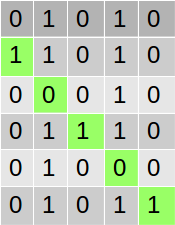
\includegraphics[scale=0.4]{figuras/pmv/notBit.png}}
    \caption{Operador de negação de bit.}
    \label{fig:operadorNegacaoBit}
\end{figure}

Para as vizinhanças da solução foram usados dois tipos de operações, uma sobre $x$ e outra sobre $y$, em $x$ foram usados 4 tipos de operações descritos a seguir, ao passo que para $y$ foram usadas duas operações, o operador de Negação de Bit (coletar um item se não estiver presente ou deixar de coletá-lo caso contrário, exemplificado na Figura~\ref{fig:operadorNegacaoBit}).
Em resumo, a combinação dos movimentos em $x$ e $y$ geram 8 vizinhanças diferentes.
Nessa abordagem, cada solução possui muitos vizinhos, sendo o total calculado pela Equação.~\eqref{eq:neighboorSize}.

\begin{equation} \label{eq:neighboorSize}
    |\Lambda(x, y)| = \frac{4nm(n - 1)}{2} + \frac{4n(n - 1)}{2} = 2n(n - 1)(m + 1) = \Theta(m\;n^2)
\end{equation}

\label{subsec:localSerach:neighborhoods}
As operações na rota $x$ possuem $\frac{n (n -1)}{2}$ vizinhos, a operação de Troca (Swap, Figura~\ref{fig:operadorSwap}) consiste de trocar cada par de inteiros no vetor, outrossim a operação 2-Opt consiste em reverter um grupo de elementos formado por cada par de inteiros do vetor.
A operação de Shift consiste de mover todos os elementos uma posição para a esquerda (Figura~\ref{fig:operadorShiftLeft}) ou direita (Figura~\ref{fig:operadorShiftRight}) dentro de um par de elementos.

\begin{figure}%
    \centering
    \subfloat[Troca]{{
        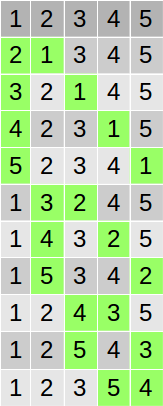
\includegraphics[scale=0.4]{figuras/pmv/swap.png}
        \label{fig:operadorSwap}
    }}%
    \qquad
    \subfloat[Inversão]{{
        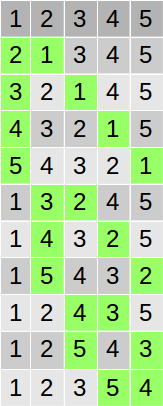
\includegraphics[scale=0.4]{figuras/pmv/inversion.png}
        \label{fig:operadorInversion}
    }}%
    \caption{Vizinhanças troca e inversão}%
    \label{fig:swapInversion}%
\end{figure}

\begin{figure}%
    \centering
    \subfloat[Shift left]{{
        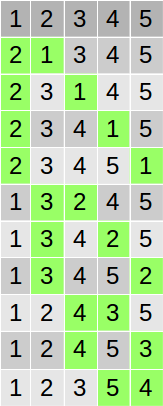
\includegraphics[scale=0.4]{figuras/pmv/shiftLeft.png}
        \label{fig:operadorShiftLeft}
    }}%
    \qquad
    \subfloat[Shift right]{{
        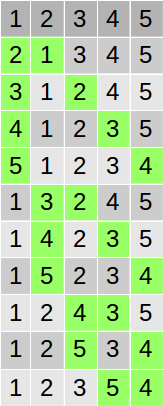
\includegraphics[scale=0.4]{figuras/pmv/shiftRight.png}
        \label{fig:operadorShiftRight}
    }}%
    \caption{Vizinhanças Shift}%
    \label{fig:shiftLeftRight}%
\end{figure}


Foi possível simular uma memória global em um dataflow pelo uso do nó de \textit{flip-flop} apresentado na Seção~\ref{subsec:flipFlop} de forma a prover uma memória para o nó \textit{man} do grafo dataflow do DVND, expresso na Figura~\ref{fig:dvndGraph}.

Conforme discutido na Seção~\ref{subsec:multiplasSaidas}, foi proposta a melhoria da biblioteca \textit{Sucuri} para que os nós de seus grafos comportem múltiplas portas de saída, sendo visto na Seção~\ref{sec:resultadosMultiplasPortas} que os resultados indicam sua eficiência para instâncias com tamanho maior ou igual a 318.

\section{RVND}

Foi discutido na Seção~\ref{sec:resultadosRVND} que em termos de melhoria na qualidade da solução não foi encontrada grande diferença nos métodos RVND em sua implementação clássica e da implementação em dataflow.

Em termos de tempo de execução houve uma pequena diferença em algumas instâncias pesando para a implementação dataflow e em outras para a implementação clássica.

\section{DVND}

No que diz respeito a comparação entre o DVND implementado em dataflow e a implementação original podemos ver que a versão clássica apresentou melhores tempos para as menores instâncias, sendo alcançado pela tempo da implementação em dataflow apenas na instância 5, de tamanho 657.
Apenas na instância 7 (tamanho 1001) o DVND em dataflow conseguiu melhorar o tempo do DVND clássico, contudo a melhoria dos resultados com o aumento do tamanho da solução indica que o mesmo possui tempo de execução mais controlado para grandes instâncias.

Em termos de valor da solução encontrada pode se ver na discussão da Seção~\ref{sec:resultadosDVND} que o DVND clássico conseguiu melhorar mais a solução inicial quando comparado à implementação em dataflow.

É importante ressaltar que tanto a implementação clássica quanto a implementação em dataflow do DVND melhoraram o tempo de execução quando comparadas ao RVND dataflow ou mesmo o clássico.

\section{GDVND}

Desta forma foi possível mostrar que o GDVND consegue diminuir a necessidade de explorar vizinhanças pois, conforme discutido na Seção~\ref{sec:gdvndTimeMan}, o tempo gasto por esse na exploração de vizinhanças é menor para as maiores instâncias, contudo carece de uma melhor estratégia para combinar os movimentos pois este está tomando uma parte significativa do tempo de execução do procedimento como um todo.

% \section{DVND} \label{sec:dvndClassico}

O \textit{Distributed Variable Neighborhood Descent} DVND concebido por~\cite{RIOS201839} utiliza múltiplas vizinhanças conforme o faz o VND (\textit{Variable Neighborhood Descent} proposto por \cite{mladenovic1997}) contudo propõe o processamento das vizinhanças de forma distribuída.
Este processamento distribuído se dá pelo escalonamento das tarefas de enumeração das vizinhanças o que naturalmente proporciona a aleatoriedade proposta no RVND.

A implementação em dataflow não pode alcançar uma grande melhoria do RVND em termos de tempo ou qualidade da solução pois o grafo se assemelha a uma cascata (veja a Figura~\ref{fig:rvndGraph}) o que não permite alcançar paralelismo, então se torna natural o uso do método DVND conforme o Algoritmo~\ref{alg:dvnd}. 
A ideia do DVND é que quando uma solução atinge um ótimo local para uma estrutura de vizinhança ainda pode existir um vizinho com melhor valor de função objetivo em uma estrutura de vizinhança diferente, destarte não necessariamente sendo um ótimo local para todas as vizinhanças
Se uma melhoria é encontrada o processo de busca é reiniciado para todas as estratégias de vizinhança.

\begin{algorithm}[htpb]
\caption{DVND clássico}\label{alg:dvnd}
\begin{algorithmic}[1]
    \Function{DVND}{Solução: $s$, Vizinhanças: $N$}
        \Let{$W$}{$\emptyset$}
        \Let{$H$}{$\emptyset$}
        \ForAll{$N_k \in N$}
            \Let{$s_k$}{$s$} \Comment{Solução atual para vizinhança $k$}
            \Let{$H_{k,s}$}{$true$} \Comment{Solução já foi enumerada pela vizinhança}
            \Let{$W_k$}{$false$} \Comment{Vizinhança aguardando solução}
            \State Chame de forma assíncrona $N^k(s_k)$
        \EndFor
        
        \While{$\exists w \in W \mid w = false$}
            \Let{$k$}{join $N^k(s_k)$} \Comment{Aguarda a resposta da vizinhança $N^k$}
            \Let{$s_k$}{Melhor solução de $N^k(s_k)$}
            \If{$f(s_k) < f(s)$}
                \Let{$s$}{$s_k$}
            \EndIf
            
            \Let{$W_k$}{$true$}
            \ForAll{$N_k \in N$}
                \If{$W_k \land \neg H_{k,s}$}
                    \Let{$s_k$}{$s$}
                    \Let{$H_{k,s}$}{$true$}
                    \Let{$W_k$}{$false$}
                    
                    \State Chame de forma assíncrona $N^k(s_k)$
                \EndIf
            \EndFor
        \EndWhile
        \Return{$s$}
    \EndFunction
\end{algorithmic}
\end{algorithm}

Considerando $ \mathcal{M} = M^{DVND} = M^1 \cup M^2 \cup \dots \cup M^k $ o conjunto com os movimentos de todas as vizinhanças usadas pelo DVND, então em termos de movimento temos que a solução $s''$ retornada a cada iteração do DVND pode ser escrita como $s'' = m_z \circ s$ com $m_z \in \mathcal{M}$ e $\widehat{m_z}(s) < \widehat{m_i}(s) \mid \forall m_i \in \mathcal{M}$.
Vale ressaltar que $\mathcal{M} = M^{DVND} = M^{RVND}$, a diferença dos métodos é que a cada iteração o RVND move para a melhor solução da vizinhança atual e no caso do DVND este move para a melhor solução entre todas as vizinhanças.

% Igor, o que acha dessa afirmação?
Numa análise em mais alto nível do RVND (Algoritmo~\ref{alg:rvnd}) e DVND (Algoritmo~\ref{alg:dvnd}), pensando-se à luz das estratégias de \textit{First improvement} e \textit{Best improvement}, o RVND enumera as soluções vizinhas da solução atual vizinhança por vizinhança até encontrar uma solução que a melhore e então retorna para a primeira vizinhança ao passo que o DVND enumera todas as vizinhanças para então optar pela solução de melhor valor.
Desta forma o RVND é uma estratégia de \textit{first improvement} no contexto de vizinhanças de solução e o DVND uma estratégia de \textit{best improvement}.


\section{Propostas futuras}

No desenvolvimento da experimentação e da análise dos resultados algumas novas hipóteses foram levantadas e são aqui apresentadas para estudo posterior.

\subsection{Testar com instâncias maiores} \label{subsec:instanciasMaiores}

No intuito de verificar melhor o desempenho do método dataflow DVND e sua escalabilidade uma prova de conceito imaginada pra ser utilizada é a realização de teste computacionais para instâncias maiores, tendo em vista a comparação de resultados com instâncias do clássico PCV.

\subsection{Decomposição de vizinhanças} \label{subsec:decomposicaoVizinhancas}

Conforme descrito na seção~\ref{subsec:metodologiaDecomposicaoVizinhancas}, as vizinhanças exploradas nos problemas não são indivisíveis, desta forma uma maneira de proporcionar maior paralelismo pode ser feita através da decomposição das destas em sub vizinhanças de forma a serem exploradas paralelamente.

Acredita-se que a decomposição de vizinhanças aliada a composição de movimentos pode proporcionar um grande ganho em termos de qualidade da solução uma convergência muito mas rápida ao serem aplicados mais de um movimento simultaneamente, melhorando assim o tempo da busca local que em geral é a etapa mais custosa em termos computacionais para o processo de solução de um problema de otimização.

% \subsection{Publicações e Cronograma}

Etapas deste trabalho já foram publicadas nas conferência International Conference on Variable Neighborhood Search (ICVNS) e publicado na edição especial do Electronic Notes in Discrete Mathematics (ENDM), também sendo publicado na conferência Parallel Programming Models (MPP), realizado em conjunto com o 32nd IEEE International Parallel and Distributed Processing Symposium (IPDPS). Existe um draft para submissão no Computers \& Operations Research, que irá englobar resultados da união de movimentos.

% ... Escrever um pouco melhor.
A etapa inicial do trabalho, apresentada no ICVNS, diz respeito ao método descrito na seção~\ref{sec:lcrvnd} e resultados apresentados na seção~\ref{sec:res_lcrvnd}.
A proposta apresentada no MPP é detalhada na seção~\ref{sec:df_dvnd} e seus resultados analisados em~\ref{sec:res_df_dvnd}.

O cronograma esperado é desenvolver a proposta e fechar antes do prazo regular do mestrado (Outubro/2018), com meta de terminar ainda em Agosto/2018 para inscrição imediata e entrada em programas de doutorado da região.
 %conclusao nao conta como capitulo

%\cleardoublepage

%configuracao do capitulo para referencia
\titleformat{\chapter}{\normalsize}{\thechapter}{5pt}{\normalsize}
\titlespacing*{\chapter}{0pt}{0pt}{1.5cm}

\addcontentsline{toc}{chapter}{\textbf{\hspace{3.1em}Referências}} %adiciona referencias não bugada no sumário

\singlespacing

\citeoption{abnt-options4}

\let\oldaddcontentsline\addcontentsline
\renewcommand{\addcontentsline}[3]{}%retira uma linha bugada de referencias do sumário
\bibliography{bin}
\let\addcontentsline\oldaddcontentsline

\end{document}
